% 12 point font, and your thesis is a ``report'' to LaTeX
\documentclass[12pt]{report}

% this enables correct linespacing and graphics inclusion via 
%``\includegraphics''
\usepackage{setspace}
\usepackage{graphicx}

\usepackage{amssymb}
\usepackage{wrapfig}
\usepackage{graphicx}
\usepackage{gensymb}
\usepackage{hyperref}
\usepackage{nameref}
\usepackage{graphicx}
\usepackage{lipsum,multicol}
\usepackage{mdwlist}
\usepackage{soul}
\usepackage{hyperref}
\usepackage{amsmath}
\usepackage{graphicx}
\usepackage[export]{adjustbox}
\usepackage[ruled,vlined]{algorithm2e}
\usepackage{algorithm,algpseudocode}
\usepackage[utf8]{inputenc}
\usepackage[english]{babel}
\usepackage{subcaption}
\usepackage[utf8]{inputenc}
\usepackage{listings}
\usepackage{xcolor}
\usepackage{subcaption}
\usepackage{enumitem}

\setlist{nolistsep}
%New colors defined below
\definecolor{codegreen}{rgb}{0,0.6,0}
\definecolor{codegray}{rgb}{0.5,0.5,0.5}
\definecolor{codepurple}{rgb}{0.58,0,0.82}
\definecolor{backcolour}{rgb}{0.95,0.95,0.92}

%Code listing style named "mystyle"
\lstdefinestyle{mystyle}{
  backgroundcolor=\color{backcolour},  
  commentstyle=\color{codegreen},
  keywordstyle=\color{magenta},
  numberstyle=\tiny\color{codegray},
  stringstyle=\color{codepurple},
  basicstyle=\ttfamily\footnotesize,
  breakatwhitespace=false,         
  breaklines=true,                 
  captionpos=b,                    
  keepspaces=true,                 
  numbers=left,                    
  numbersep=5pt,                  
  showspaces=false,                
  showstringspaces=false,
  showtabs=false,                  
  tabsize=2
}

\lstset{style=mystyle}
\renewcommand{\lstlistingname}{Code Block}


% leave 1.5in margin to the left and 1in margin to the other
% sides. Don't print page number in the margin (but rather above it)
\setlength{\textheight}{8.63in}
\setlength{\textwidth}{5.9in}
\setlength{\topmargin}{-0.2in}
\setlength{\oddsidemargin}{0.3in}
\setlength{\evensidemargin}{0.3in}
\setlength{\headsep}{0.0in}

% Start to write
\begin{document}


\newcommand{\brk}{\vspace*{0.18in}}

% No page number on the title page
\thispagestyle{empty}

% Center the whole title page
\begin{center}

\brk

% Large font and bold face for the headline. Try to keep it at one or
% two lines. Headlines over two lines will mess up the spacing, and you have to
% manually finetune it. Note that the line break in the SOURCE CODE
% does not affect the line breaking in the output file. If you want
% hardcoded line breaks, you have to mark them with a double backslash (\\)

   {\large 
	\textbf{
	Development and an Lower Limb Exoskeleton and Simulation Framework 
	}
   }


\brk
by

\brk
% insert your name here. 
Nathaniel Goldfarb


% All this is constant:
\brk\brk
A Thesis

\brk
Submitted to the Faculty

\brk
of the 

\brk
WORCESTER POLYTECHNIC INSTITUTE
	
\brk
In partial fulfillment of the requirements for the

\brk
Degree of Doctor of Philosophy

\brk
in

\brk
Robotics Engineering

% Adjust this to your preferred month and year
\brk
May 2000

\end{center}

	
\vfill
APPROVED:

\vspace{0.25in}
\rule{3in}{0.8pt}

% Change this to your favorite CS professor.
Professor Gregory Fischer,Thesis Advisor

\vspace{0.25in}
\rule{3in}{0.8pt}

% This is also constant :)
Professor Karen Troy,  Committee Member


\vspace{0.25in}
\rule{3in}{0.8pt}

% This is also constant :)
Professor Jie Fu,  Committee Member


\vspace{0.5in}
\rule{3in}{0.8pt}

% This is also constant :)
Professor Berk Calli,  Committee Member

% end of titlepage
\newpage

% This is the command for doublespacing when you use the setspace
% package
% Please do NOT use \baselinestretch, this will mess up everything,
% cause earthquakes, tornados and lots of questions for me...
% If you need a singlespaced paragraph (BAD STYLE!!!), use
% \singlespacing or \onehalfspacing and enclose it together with the
% paragraph in braces {\singlespacing This is my text... blah blah blah}
%
\doublespacing

% Now you can start to be creative.
% First, you need an abstract.
% Fortunately, LaTeX has thought of that, so it's very easy:
\begin{abstract}
Still working on this

\end{abstract}

% From here on, we need Roman page numbers according to the library
% regulations. So let's assign those.

\pagenumbering{roman} % or {Roman} if you like them capitalized


\begin{center}
	\textbf{Acknowledgements}
\end{center}

blah

\clearpage

\begin{center}
    \textbf{Dedication}
\end{center}
This is dedication to my Great Uncle Lawrence "Larry" Solomon (June 28, 1949 to March 3, 2007) who I named the exoskeleton after "Legged Articulated Robotic Rehab Exoskeleton(LARRE). Larry suffered a C6 SCI in 1968 at 19 yrs old while practicing a gymnastics long vault at Springfield College. He lived a full and inspiring life. Within months of his accident, Larry was asked to help inspire the other young people with SCI injuries with his positive attitude. He never let his SCI injury stop him from doing anything. He went on to get a Doctorate in Education Administration before the days of computers and all the technology available today to people with SCIs and served on the Presidential Council  of the Americans with Disabilities Act. Larry was a great husband, father, brother, and uncle. He made everyone around him feel like they were the most important person in the room. Although, I never had a chance to know him very well, I have been told that he was one of the most inspirational people you could ever know.
\begin{center}
\Large
\textbf{I DID IT!}     
\end{center}

\clearpage

% The next thing is the Preface (``Acknowledgements'').
% No standard environment for that, so we'll format it by hand.
%


% P.S. You don't have to add me to the acknowledgements for providing 
% this file :)

\clearpage


% Now comes the Table of Contents, really easy in LaTeX. you never
% have to worried about it. (Think of all the hours you would
% have wasted in Word getting this thing updated without crashing
% the system) :).

\tableofcontents

% THAT'S IT. REALLY. Everything else is automatic. No formatting, no headline.
% All predefined.

% Now - just as easy - the List of Figures.
% This will catch all objects enclosed in \begin{figure}\end{figure}
% statements.
\listoffigures

% There is also a list of tables, if you have any.
% This will catch all objects enclosed in \begin{table}\end{table}
% statements.
\listoftables


% And we need a clear separation between preface and text, otherwise
% the numbering gets confused.

\clearpage

% And now - tataa - the text.
% This is the place to become really creative.

% From here on, we need arabic numbering again and we need to start
% from 1.

\pagenumbering{arabic}
\setcounter{page}{1}


\maketitle
% \chapter{Introduction}

Exoskeletons are a branch of human-machine robotic systems. Many different exoskeletons provide different functionality levels and are designed to meet different requirements. Rehabilitative lower-limb exoskeletons enhance gait motion for people with reduced lower body control; this is an essential field of study for spinal cord injuries or other neurological injuries. Lower limb exoskeletons provide a method of enhancing and providing external support to the person. Increasing the research in this field will improve the lives of people. Unfortunately, exoskeleton research is usually proprietary, expensive, and requires a vast knowledge of engineering and biomechanics. This research aims at solving several problems currently in the field and providing open-source tools for exoskeleton development and research. This work is divided between the development of the controllers and open-source tools. The controller will learn from demonstration and provide assistive torques to the person wearing the exoskeleton.


This work focused on developing a simulation framework and a controller for a robotic lower-limb exoskeleton. The aim and functionality of these exoskeletons are not targeted for assistive, recreational, or industrial use but rather intended for rehabilitation use. Therefore, the exoskeleton's controls will not be designed to handle arbitrary disturbances and collisions with the environment. It is assumed that the controllers are being used in a safe and open environment to avoid obstacles, though the techniques presented here may be adapted to enhance exoskeleton performance and interaction with the user in such environments. The controller will use human motion capture data to generate gait motions and control the exoskeleton joints. The contributions are separated into implementation and conceptual contributions. The implementation's contributions enabled the testing and development of the conceptual development. The contributions are summarized below and will be discussed throughout the paper. 

\section{Primary Conceptual Contributions}
\begin{enumerate}[wide, nosep, labelindent = 0pt, topsep = 1ex]
     \item A trajectory controller based on human demonstration mocap data. A method using mocap data will be presented to train a generalized trajectory for an exoskeleton to follow a learned trajectory; this allows for generalized gait motion that does not have to be retrained for each person. 
    \item  Kinematic and dynamic models of a lower limb exoskeleton and a human wearer and their interactions. The exoskeleton will have sensors to measure the joint kinematics and the human torque to allow for cooperative controllers. The framework allows for the human effort commands to be sent to the system along with the typical robotic exoskeleton commands. 
    \item An optimal controller procedure using human demonstration for minimizing the control input. A method will be presented using optimal control theory and human motion to develop a controller. This controller combines learning from demonstration and optimal control for a controller optimized from the collection of training data to the torque generation. 
    \item Cooperative controller for shared control of a lower limb exoskeleton to handle the reduced torque of the person. The simulated torques applied to the model to represent the human wearer will be generated using a closed-loop controller that will be limited and time-varying in the amount of torque it can generate. The exoskeleton controller will account for the fatigue and reduction of torque. 
    \item Sensitivity analysis and tuning method for an Admittance Sliding Mode Controller to automatically tune the controllers' parameters. The sensitivity analysis shows the controller parameters' relative importance and their effect on the optimization cost function.  
\end{enumerate}

\section{Primary Implementation Contributions}
\begin{enumerate}[wide, nosep, labelindent = 0pt, topsep = 1ex]
    \item Open source toolkit for analyzing and parsing motion capture data with tools for gait analysis. This toolkit contains tools to handle marker data and rigid bodies.  
    \item Open source hardware of the lower limb exoskeleton for passive data collection. The exoskeleton will have sensors for sensing the motion and be passive purely for data collection.
    \item A collection of joint data from a range of subjects, climbing stairs and walking, will be released open-source for community use.  
    \item Implementation of an exoskeleton and human simulation for testing and implementation of the controller assuming no ground collisions. 
    \item A controller will be implemented that integrates the human and exoskeleton for a cooperative controller in simulation. The controller will measure the human torque generated by a closed-loop controller while the exoskeleton provides the additional torque to follow a trajectory.  
\end{enumerate}
\chapter{Background}

\section{Lower Limb Weakness and Rehabilitation}
\subsection{Introduction}
Rehabilitation robotics systems are now used to treat different conditions. 
Two prominent conditions are spinal cord injuries (SCI) and strokes. While SCI and strokes are different medical conditions, they are highly traumatic to the body and cause motor damage to one or all limbs depending on the severity of the injury and the response of emergency intervention. Similar rehabilitation methods and robotic tools are currently being examined as a treatment for both injuries.  


\subsection{Spinal Cord Injuries}
In the United States, approximately 282,000 people living with Spinal Cord Injuries (SCI) with approximately 17,000 new cases each year \cite{national2016facts}. SCI results in loss of motor function and sensor function. The amount of loss functionality depends on the injury level. As the injury location goes up the spinal cord, more functionality is lost, as shown in \autoref{fig:SCILevels}. The injury levels defined by the  American Spinal Injury Association (ASIA)  scale is as follows A–B; cervical (C7–C8) or thoracic (T1–T12) according to ASIA guidelines \cite{kirshblum2011international}. Accordingly, injuries level between C7-T12 are identified as the target requirement for lower limb exoskeleton studies \cite{esquenazi2012rewalk}. 

The injury level results in one of many classifications that define their functional ability. Paraplegia results in impairment of the trunk, legs, and pelvis. Tetraplegia results in the upper and lower body's impairment, including the arms, trunk, and other organs. An incomplete SCI is when there is some remaining sensory or motor function below the injury level.  Incomplete injuries, there is no motor or sensory functionality below the injury level. 

The cost of lifetime treatment is between \$500k -\$2M depending on the injury level \cite{mcdonald2002spinal}. This cost includes the initial cost immediately after the injury and the treatment of secondary health side effects.  

 

\begin{figure}
    \centering
    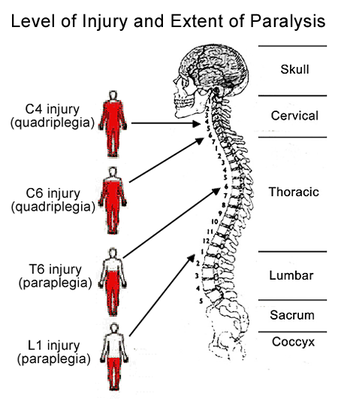
\includegraphics[scale=0.6]{images/background/SCI.png}
    \caption[Levels of SCI]{Levels of SCI \cite{sadaka2012bradycardia}}
    \label{fig:SCILevels}
\end{figure}

A secondary health side effect is a physical or psychological health condition caused by the disability \cite{jensen2012secondary}.  These side effects include the decrease in the bone density of the femur, decrease in blood pressure, and reduced muscle mass \cite{haisma2007complications} \cite{hitzig2010understanding}. These side effects result in a significantly reduced Quality of Life (QoL) of the person.  	\cite{craven2012impact}. Prevention of these side effects through rehabilitation will help increase the QoL and overall health of the person.  




\subsection{Strokes}
Strokes are a global health crisis with approximately 800,000 occurrences each year in the United States and is a leading cause of death worldwide \cite{george2017cdc} \cite{murphy2020stroke} \cite{feigin2015update}. While strokes have been decreasing worldwide, the rate of stroke in younger people (18-54 years old) has risen. The expected cause is increased hypertension, diabetes, lipid disorders, obesity, and tobacco use. 

A stroke is a medical condition where the blood vessels to the brain get blocked or burst; this means that the brain cannot get the necessary blood flow, and the tissue begins to die. There are broadly two different types of strokes \cite{perna2015rehabilitation}; ischemic strokes and hemorrhagic strokes as shown in \autoref{fig:strokes}. An ischemic stroke is caused by obstructed blood vessels. This type of stroke accounts for approximately 85\% of all strokes. A hemorrhagic stroke is caused when the blood vessels of the brain burst.  

\begin{figure}
    \centering
    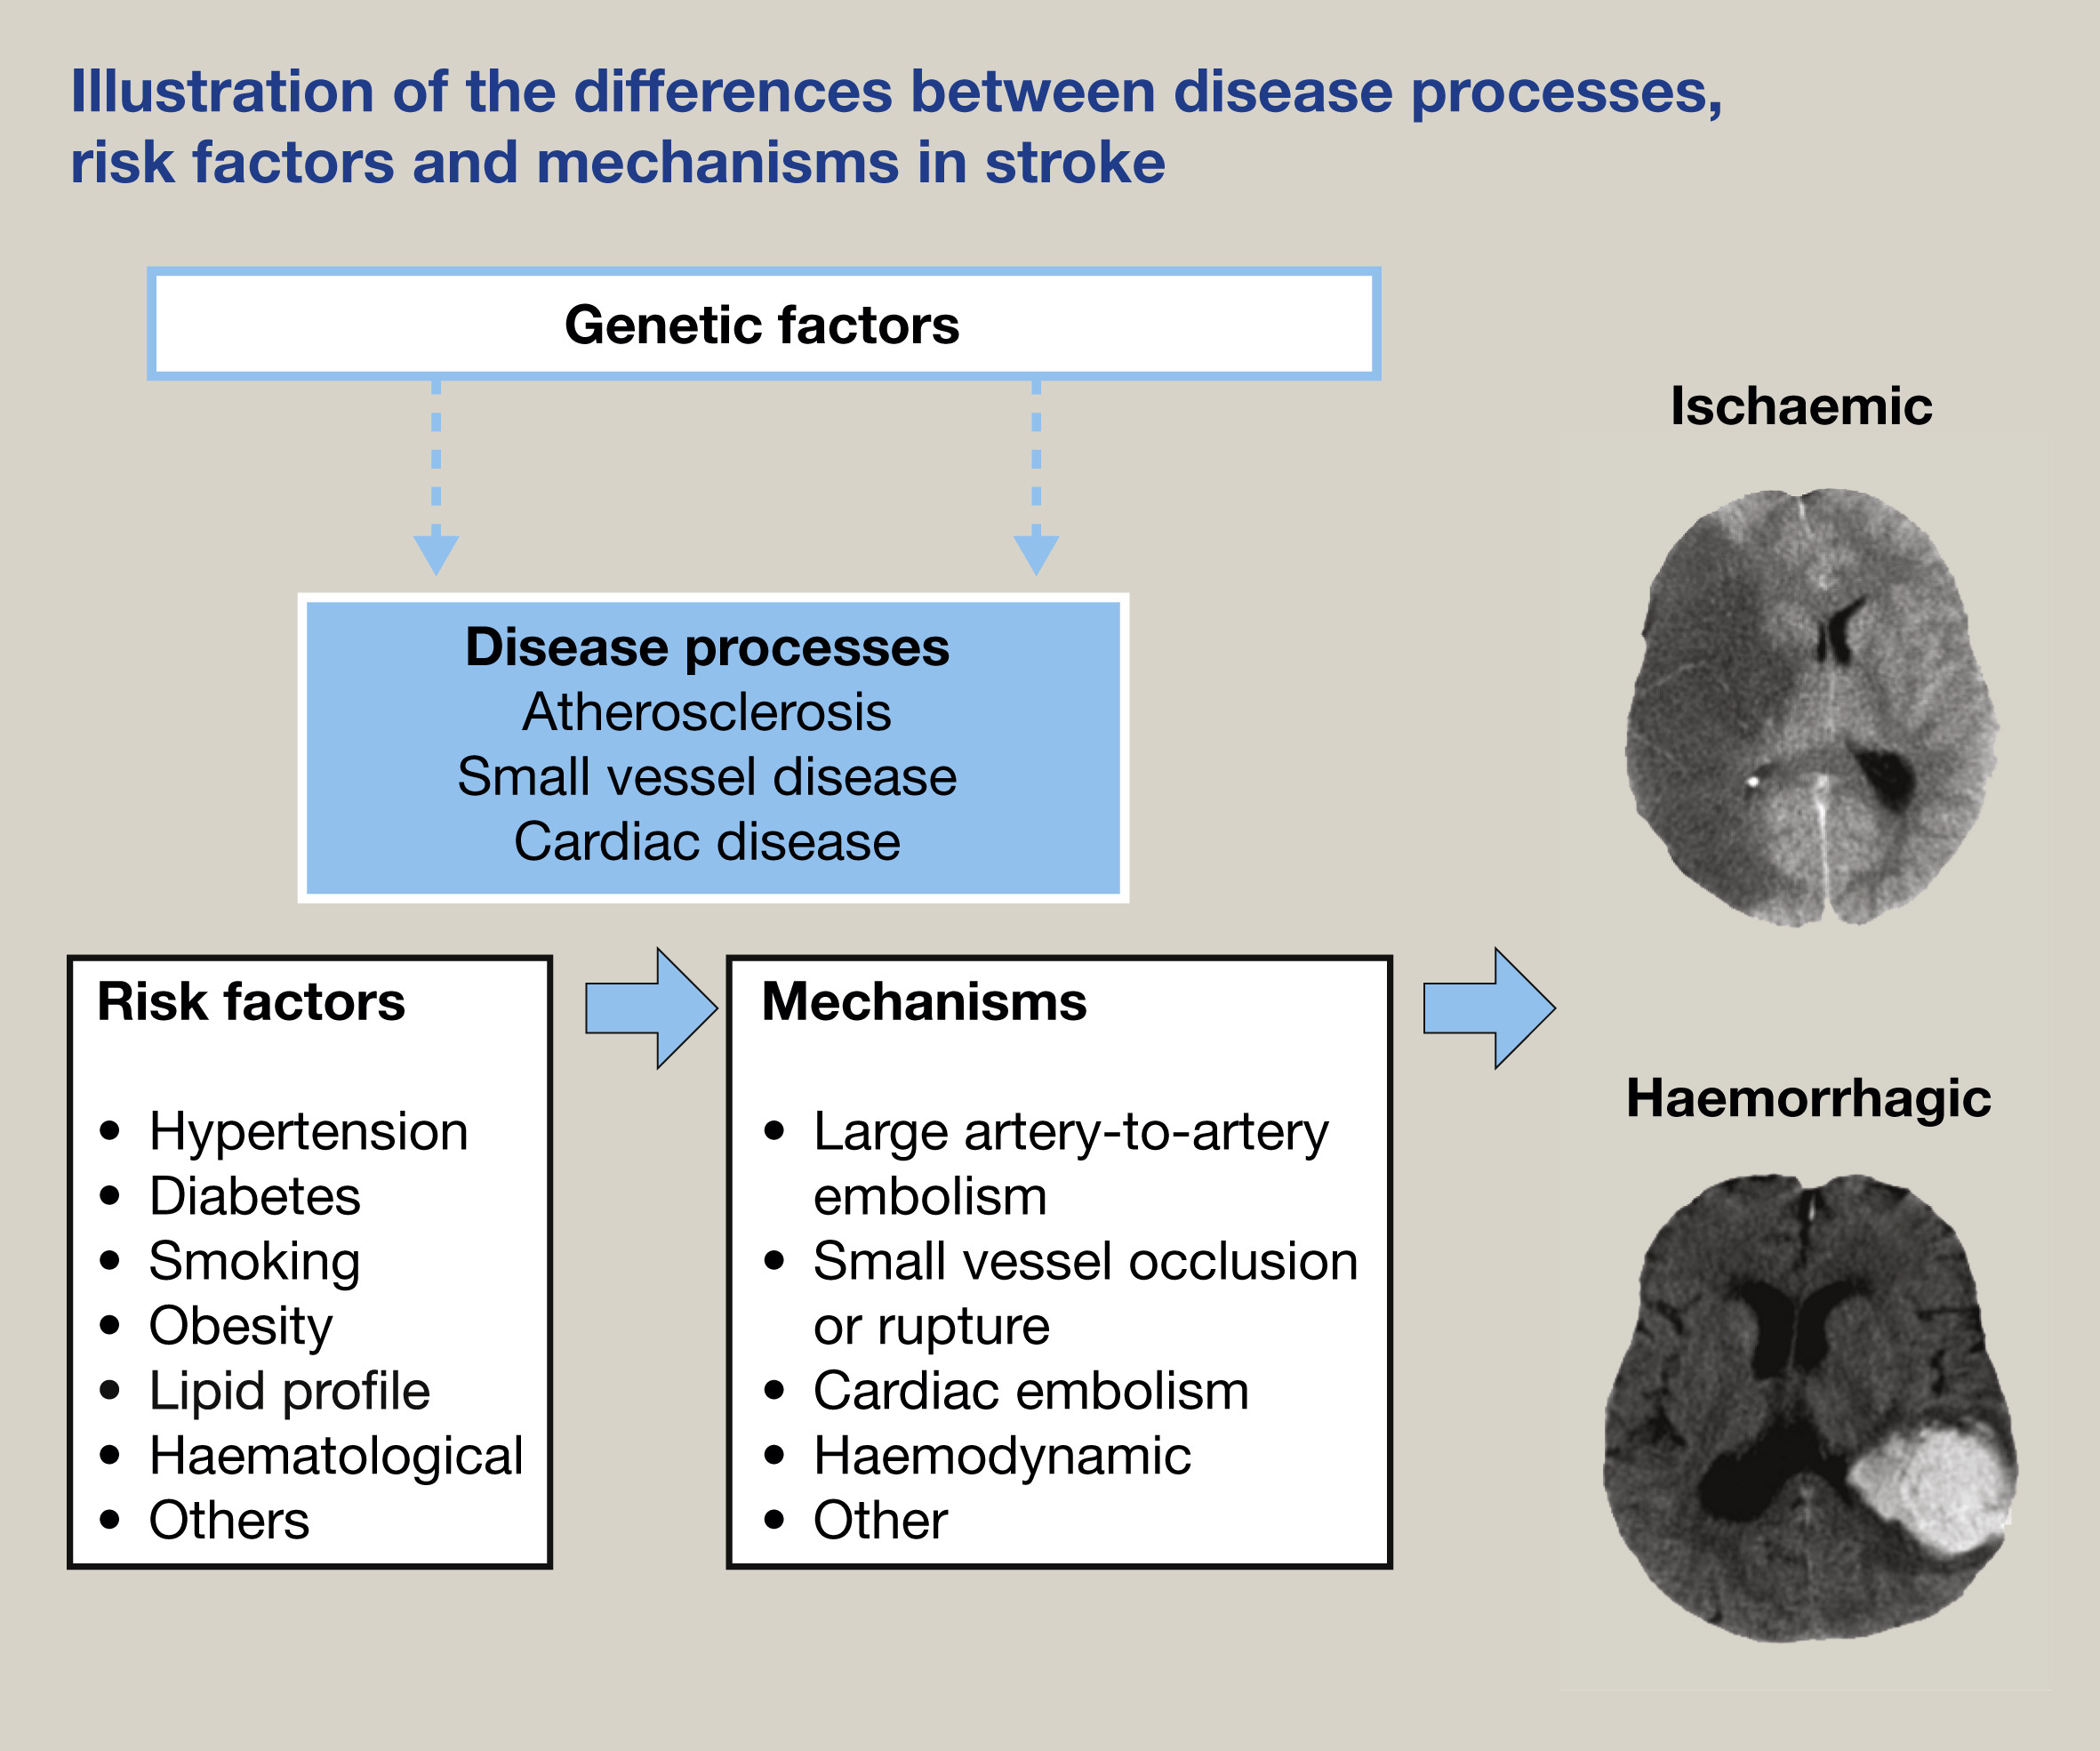
\includegraphics[scale=0.85]{images/background/stroke.jpg}
    \caption[Ischemic strokes and Hemorrhagic strokes]{Ischemic strokes and Hemorrhagic strokes \cite{murphy2020stroke}}
    \label{fig:strokes}
\end{figure}


It is crucial to receive treatment immediately after a stroke. Each minute causes more tissue and brain damage to occur \cite{saver2006time} resulting in about 1.9 million neurons per minute; this can result in both upper and lower limb weakness along with other cognitive complications \cite{pennycott2012towards}. Emergency treatment to restore blood flow has been shown to improve outcomes which are essential for getting the patient back to normal life with less loss of functionality \cite{goyal2016endovascular}.  



\subsection{Rehabilitation}
\label{sec:rehab}

 Rehabilitation is critical for regaining lost functionality and gaining independence to live a long, fruitful life; this does not mean that motor and sensory functionality will be completely or partially recovered but to reduce other medical side effects, have the ability to navigate the world and complete daily living activities (ADL), and improve QoL. QoL includes the betterment of the mental and emotional state of mind while mitigating the injury's physical side effects. By increasing the physical ability through physical rehabilitation and exercises, the person's QoL is improved \cite{noreau1995spinal}. Successful rehabilitation should teach a person how to physically navigate the world and give the person the motivation to interact with their community \cite{hammell2013spinal}.
 
 
 The rehabilitation process should start immediately after a traumatic injury. Most of the recovery progress is within the first year after the injury; this has been shown to have better long-term outcomes than delayed therapy \cite{scivoletto2005early} \cite{piepmeier1988late}.  The constraints of the wheelchair cause numerous long-term health problems. Being confined to a seat all day causes the leg muscle to atrophy \cite{castro1999influence}, the leg bones become weak \cite{goemaere1994bone} without a gravitational load, and get pressure sores \cite{wall2000preventing}. The complications lead to significant discomfort for the person and can lead to bone fractures, and heart problems \cite{giangregorio2006bone}.  
 
 The primary cause of these health side effects can be prevented by exercise and loading the leg bones. Functional Electrical Stimulation (FES) is a rehabilitation tool used to stimulate muscle activation  \cite{quintero2012preliminary}. There are several benefits of using FES for SCI rehabilitation; clinical outcomes, fitness benefits, and functional gains \cite{hamid2008role}. FES has been used to allow people to stand, walk, and use a cycle\cite{mazzoleni2013fes}. All of which have measurable rehabilitation and health benefits. FES's main complication and limitation is muscle fatigue \cite{karu1995reducing}. Only using FES  does not provide any structural support to hold up the person. FES can be supplemented by using mechanical structures to support the patient and add a layer of safety. 
 
A mechanical orthosis helps the patient stand upright and walk and reduce and reverse some of these side effects \cite{palermo2017clinician}. The first systems were simple mechanical devices that assisted in ambulatory management, including Knee-Ankle-Foot-Orthosis (KAFO) or hip-KAFO (HKAFO). These devices performed poorly and required high metabolic energy expenditure \cite{del2012review}. As technology increased, these devices were made active using robotic technology, decreasing the patient's demand. These devices are discussed further in \autoref{sec:ExoBack}. The combination of FES and an active exoskeleton is called a hybrid exoskeleton \cite{ha2012enhancing} \cite{alouane2019hybrid}. 

Robotic exoskeleton-based rehabilitation does not necessarily produce better functional outcomes than traditional rehabilitation. However, one of the benefits of robotic rehabilitation is that it reduces the load on the therapist. Robotic exoskeletons can offer gait and balance training which is more than a single therapist might offer \cite{guidingLeg}, both the patient and the therapist reap the benefits. The patient receives gait training that follows an exact and repeatable motion, reducing the physical demand on the therapist, allowing them to focus more on patients and create more personalized care.  


A great deal of research has been published on the rehabilitation benefits of robotic rehabilitation. It has been used for post-SCI rehabilitation and post-stroke rehabilitation. For SCI, lower limb exoskeletons have had a significant focus in recent years, with several studies conducted \cite{esquenazi2012rewalk} \cite{zeilig2012safety} \cite{6876184}. Similar studies were conducted for stroke rehabilitation; however, it should be noted that upper arm exoskeletons have also been examined \cite{chang2013robot} \cite{ho2011emg}. 

The most common tests and metrics with robotic lower limb exoskeletons are; 6-minute walk test (6MWT) and the 10-meter walk test (10MWT) \cite{amatachaya2014concurrent}. Research has shown improvements in all the measured criteria. In general, increased walking velocity, walking distance, and endurance. The amount of improvement varied from subject to subject and was dependant on many factors, including injury level.   
\section{Robotic Exoskeletons}
\label{sec:ExoBack}
\subsection{Introduction}

A powered exoskeleton is a wearable robotic system that offers assistive torques and increased structural support. It is an example of a Human-Machine-Interface (HMI). There has been increased interest in exoskeleton research as robotic technology as increased and has become more widespread \cite{aliman2017design} \cite{chen2016recent} \cite{mertz2012next} \cite{gardner2017review}. Robotics technology has allowed smart systems to sense movement, provide feedback, and use more accurate models to produce smooth trajectories \cite{5462998}. As sensors and actuators have become more accurate and smaller, they can create lighter and more powerful exoskeletons. However, this also increases the technological difficulty in designing and building an exoskeleton. Over the years, exoskeletons have moved from simple mechanical structures to wearable robots that can sense intention and act independently. Two of the most common exoskeleton types currently being used are treadmill-based systems and overground-based systems \cite{diaz2011lower}.

Unfortunately, the world is designed by and for able-bodied people; not all places are wheelchair accessible or easily accessible for physically challenged people. In our everyday life, we walk upstairs, reach for items on high shelves, go through narrow doorways, and talk to people at eye level \cite{welage2011wheelchair}. All of these ADLs are challenging when confined to a wheelchair. Exoskeletons allow people to walk upright and live a more "normal" life. 


\subsection{Orthosis}

An orthosis is a wearable mechanism that can provide structure or power to a joint, designed to be passive or active, and have built-in sensors. A smart orthosis with actuators is classified as a robotic orthosis. Research has produced a large amount of literature on different orthotic mechanisms. Each joint in a person has different requirements and requires different technology to support and provide supplemental power. Two of the most active research areas are knee orthosis and ankle-foot orthosis. 


Several different knee orthoses designs for exoskeletons are responsible for providing power to the knee and preventing buckling. Knee orthoses are normally designed as a brake or a clutch system. Elliott \textit{et. al} presented a clutch spring knee joint for a running exoskeleton shown in \autoref{fig:runexo} \cite{elliott2014design}. This system engages and disengages the leaf spring based on the gait phase. The system holds approximately $190Nm$ with a mass of $0.710Kg$

Farris \textit{et. al} introduced a new type of brake called Wafer Disc Brakes for rehabilitation \cite{farris2009design}. The brake operates in a normally closed state that remains engaged even during a power failure, thus enabling the user's safety. The brake uses a series of stacked high-strength wafers where the stator and rotor discs are placed alternating with a relatively small distance. A motor is coupled to the center shaft. It produces a compressive force exerted via a ball screw to the discs when activated. This setup allows the brake to hold a static torque of $73Nm$. The Austin exoskeleton project, a version control technique based on a Wrap Spring Clutch/Brake mechanism, was inherently executed to produce multiple knee joints.
 
 
 \begin{figure}[h]
    \centering
    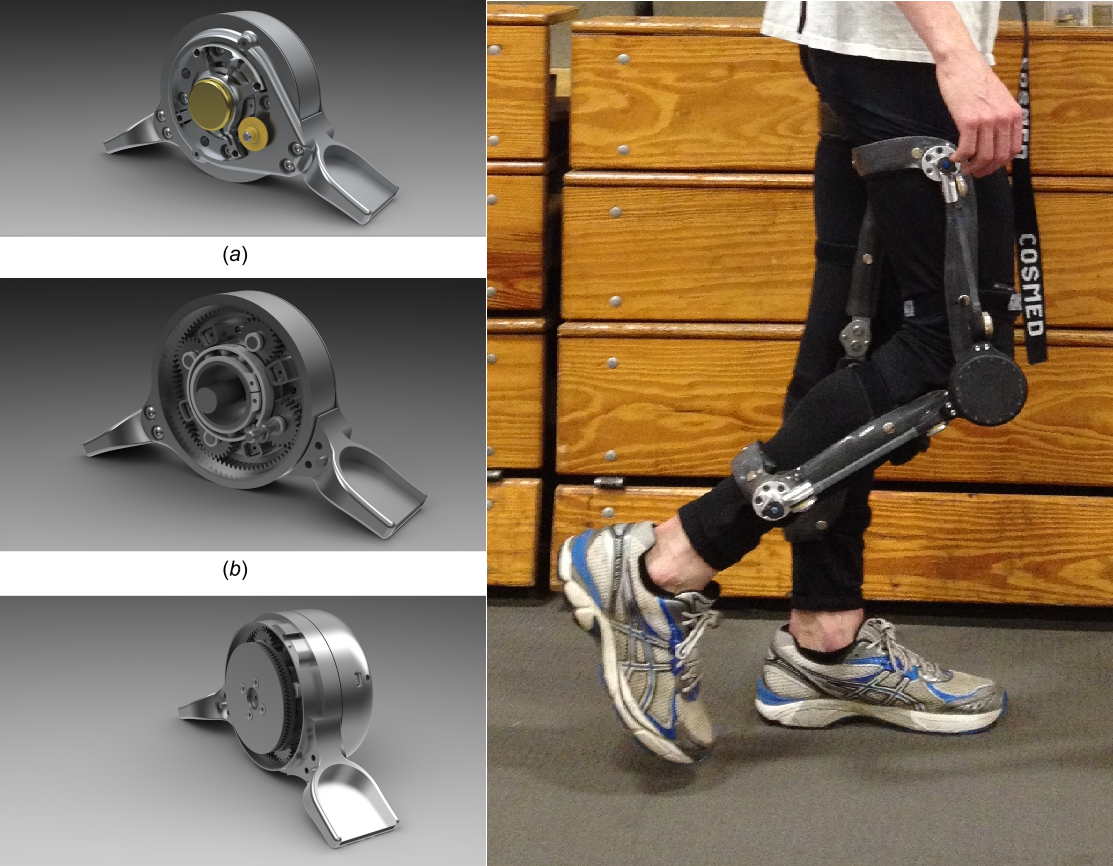
\includegraphics[scale=0.30, frame]{images/background/clutch.png}
    \caption[Clutch Spring Knee]{Clutch Spring Knee Exoskeleton for Running \cite{elliott2014design}}
    \label{fig:runexo}
\end{figure} 


Ankle-foot orthoses (AFO) designs focus on either fully active ankle actuation or on entirely restricting the motion of the foot itself. The majority of these designs are categorized as either solid ankle-foot orthoses (SAFO) or dynamic, advanced ankle-foot orthoses (DAFO) \cite{poweredAFOChina2012_6308213}. SAFOs are fully static devices designed to keep the user's foot locked at a fixed position \cite{staticAFO_6610673}. These typically consist of a single piece of plastic. DAFO devices, in contrast, consist of multiple components attached around a single adjustable hinge joint in order to avoid restricting the full range of motion of the foot \cite{poweredAFOChina2012_6308213}. DAFO designs can either be passive, non-powered devices, actively powered electrical components, or passively powered non-electrical means \cite{RussellEsposito2018}. Both actively-powered and passively-powered devices work to provide some means of controlling the angular position of the ankle throughout the gait cycle \cite{poweredAFOChina2012_6308213} \cite{actAFOFricCTRL} \cite{pneumaticAFO2009}. \autoref{fig:PAFO devices} shows some examples of different types of Powered AFO devices. An actively-powered system provides torque to aid in walking and adds mass and cost to the system.

\begin{figure}[h!]
    \centering
    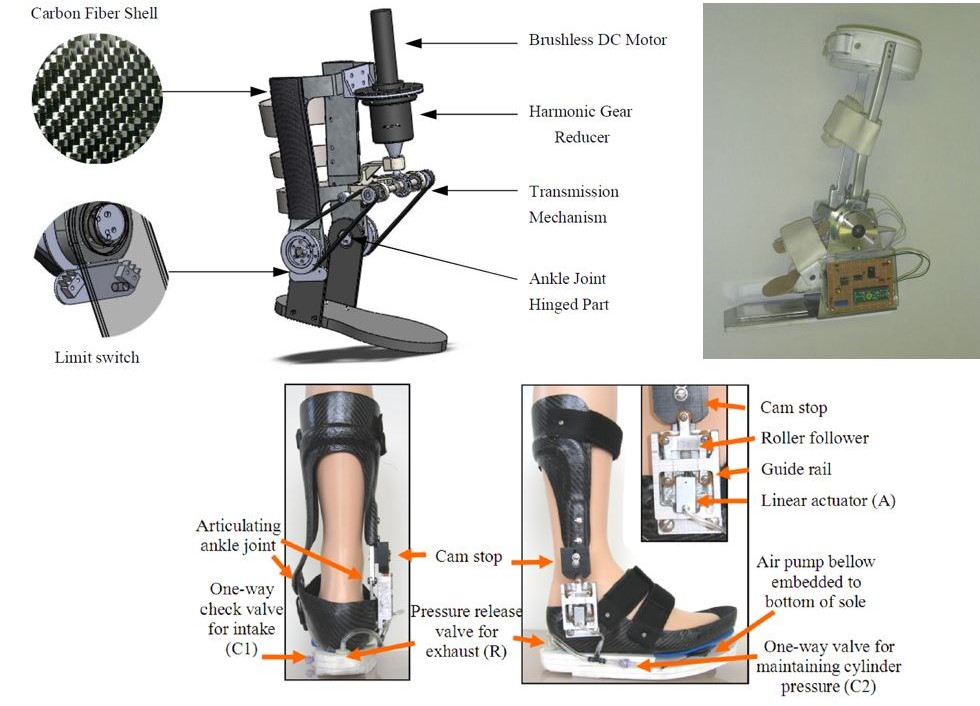
\includegraphics[scale=0.30]{images/background/PAFO_designs.JPG}
    \caption[Active v. Passive PAFO]{Various PAFO devices throughout the literature. (Top-Left) Active-PAFO (aPAFO) device that uses a motor-driven belt-chain set-up to control ankle tilt \cite{poweredAFOChina2012_6308213};  (Top-Right) aPAFO device that uses powered DC motor attached directly to the ankle-joint to control the wearer's foot \cite{actAFOFricCTRL};  (Bottom) passively-powered PAFO (PAFO) device powered by air pump attached to the sole \cite{pneumaticAFO2009}.}
    \label{fig:PAFO devices}
\end{figure} 

\subsection{Treadmill Exoskeletons}

Treadmill gait trainers, also called Body Weight Support Treadmill Training (BWSTT) or Robotically Assisted Gait Training (RAGT), typically consist of a treadmill integrated with a harness to support the person in the system and a robotic gait trainer to move the person's legs. These systems provide ample safety for the person by using a gantry and harness system to prevent falling during a trial. The control of the joint motors syncs to the treadmill's speed; this enables control of the gait speed.
 
The \textbf{Lokomat}\footnote{Hocoma AG, Industriestrasse 4, CH-8604 Volketswil, Switzerland } is a popular treadmill based exoskeleton \cite{jezernik2003robotic}. The system consists of a treadmill, a robotic orthosis, a suspension system, and two PCs. It is a 4-degree system (hips and knees). The Lokomat can be adopted for stroke and SCI patients. An adaptive PD controller controls the joints of the exoskeleton. Several well-documented studies document the benefits of the Lokomat for rehabilitation as discussed in \autoref{sec:rehab}.
 
 
\begin{figure}[H]
    \centering
    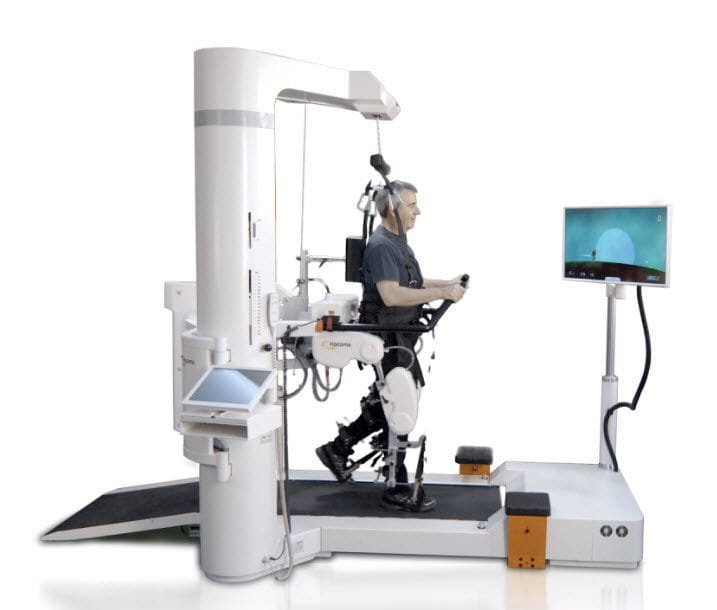
\includegraphics[scale=0.25]{images/background/loko.jpg}
    \caption[Lokomat Exoskeleton]{Lokomat Exoskeleton}
    \label{fig:loko}
\end{figure} 
 
The \textbf{Lopes} exoskeleton is another BWSTT exoskeleton. This system also uses an impedance controller to allow positional control with force interaction. This system has 8 DoF to allow hip, knee, up/down, forward/backward, and sideways freedom. Unlike many other rehabilitation exoskeletons, the actuators utilize Bowden cables for joint movement \cite{veneman2007design}. 

\begin{figure}[H]
    \centering
    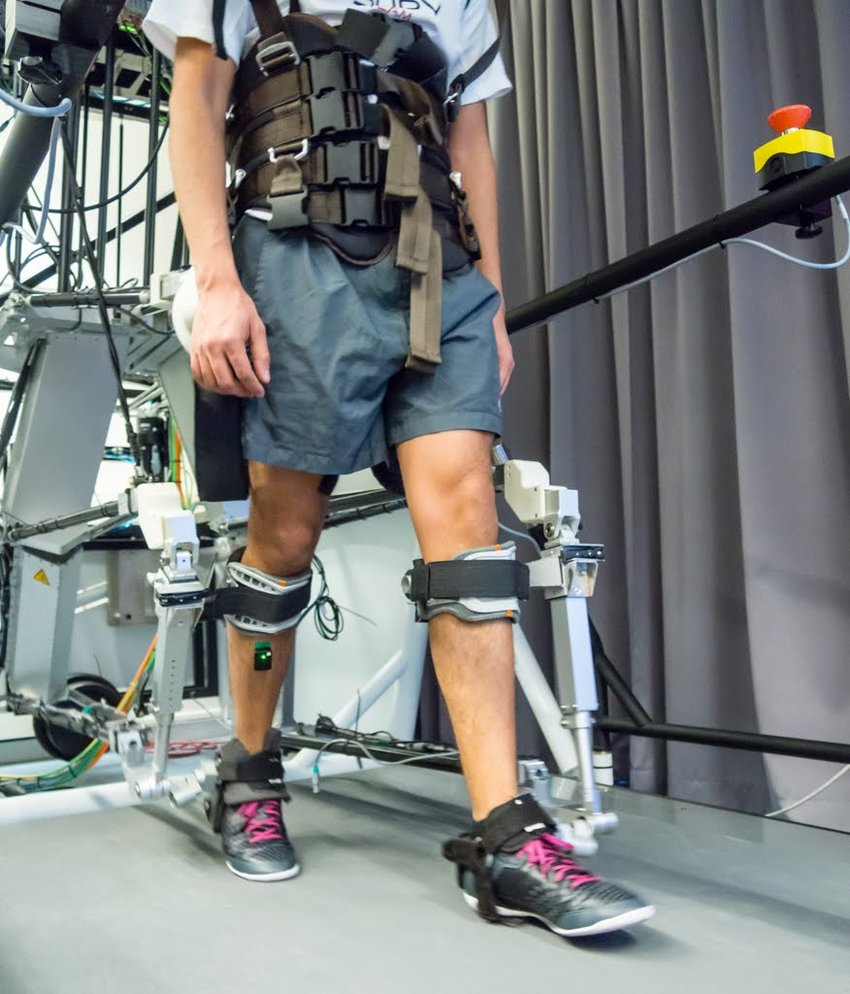
\includegraphics[scale=0.6]{images/background/A-subject-walking-with-LOPES-II-exoskeleton.jpg}
    \caption[LOPES Exoskeleton]{LOPES Exoskeleton \cite{lopes}}
    \label{fig:lopes}
\end{figure}


The disadvantage of this system is that it is not mobile. It constrains the subject to the treadmill, which does not allow for rehabilitation to involve non-level ground walking, sit-to-stand (and vice-versa), and stair climbing. Due to the support of the harness, BWSTT does not address balance recovery. It also does not have a home mode, allowing for improved daily living. Overground exoskeletons address this problem by removing the gantry systems and embedding all the actuators and controllers into the exoskeleton allowing for the freedom to move beyond a treadmill's confines.

\subsection{Overground Exoskeletons}

Several overground walking exoskeletons have been researched and developed in the past few years and have gained wide popularity. These allow for more freedom for the therapist to design protocols and represent a more realistic representation of real-world ambulation \cite{8110705} since the person is not attached to a restrictive gantry; instead, all the power and control is on-board, allowing the person to move freely in the environment. The system needs to be able to carry itself and the person. This freedom allows for movement on uneven ground and stairs. The disadvantages of these systems are that they are limited by on-board power and have to account for the system's mass. A typical design feature throughout most of the overground exoskeletons are Maxon motors\footnote{Maxon, 125 Dever Drive Taunton, MA 02780, United States}, and Harmonic gearboxes\footnote{Harmonic Drive LLC, 89 Cabot Ct # A, Hauppauge, NY 11788} \cite{bortole2015h2} \cite{aliman2017design}. The patient typically uses crutches while walking to help support the person's upper body. On average, these systems cost about \$100k \cite{rupal2017lower}.


The \textbf{BLEEX} is one of the earliest exoskeletons on the market \autoref{fig:esko} shows the current version of the BLEEX exoskeleton. The major difference between this exoskeleton and the other exoskeletons discussed in this paper is that the BLEEX design increases the load that people can carry; this was needed for military applications to help soldiers carry a substantial amount of mass. It is nearly anthropomorphic but does not quite match a person's joints. It has pure rotation joints for the knee, and ball joints for the hip ankle \cite{chu2005biomimetic}\cite{zoss2006biomechanical}. The BLEEX exoskeleton focused on using clinical gait analysis for the joint design. By studying human gait motion, they were able to find the necessary design parameters for the exoskeleton, including the torques and joint ranges \cite{zoss2005mechanical}. Commercially the BLEEX became the \textbf{Ekso} exoskeleton \cite{zoss2016human}. This system cost around \$100,000 \cite{nichols_2018}. 


\begin{figure}
    \centering
    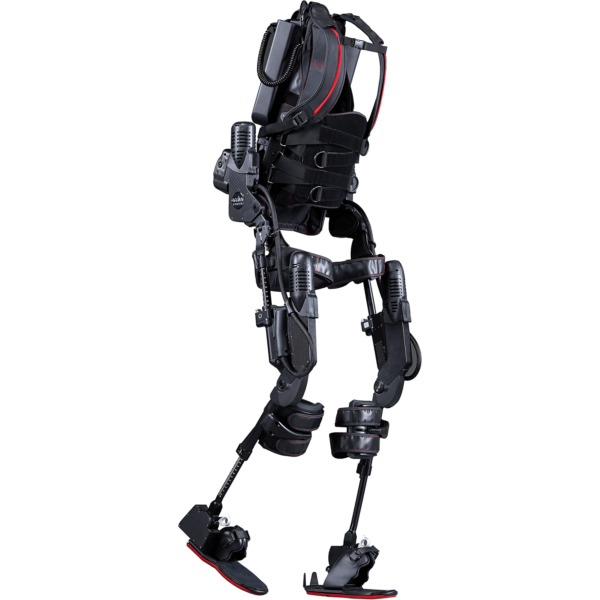
\includegraphics[scale=0.38]{images/background/ekso.png}
    \caption[Esko Exoskeleton]{Esko Exoskeleton \protect\footnote{\url{https://secureservercdn.net/72.167.25.126/045.a06.myftpupload.com/wp-content/uploads/2016/08/ekso_gt-product-image-600x600.png}}}
    \label{fig:esko}
\end{figure}


The \textbf{Rewalk}\footnote{ReWalk Robotics, Inc.
200 Donald Lynch Boulevard Marlborough, MA 01752
USA} exoskeleton is another popular rehabilitation exoskeleton on the market. \autoref{fig:rewalk} shows an image of the Rewalk. This exoskeleton has powered hips and knee joints,  the ankle joints are passive within shoe ankle support,  the control system is a closed-loop using the sensor suite to control the motors, and the body's trunk is supported with back support. The exoskeleton has several modes: sit-to-stand, stand-to-sit, up the stair, down the stair, and walking. The control of the exoskeleton is left to the user using tilt sensors in the trunk. Leaning forward tells the controller to start the walking progress  \cite{zeilig2012safety}. It is currently utilized for both inpatient therapy and at-home use. Several well-documented studies document the benefits of the Lokomat for rehabilitation as discussed in \autoref{sec:rehab}. \cite{esquenazi2012rewalk}. The home cost of the exoskeleton is approximately \$70,000 \cite{wolff2014survey}. 


\begin{figure}[H]
    \centering
    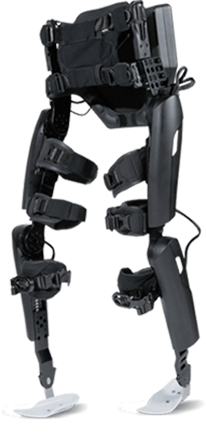
\includegraphics[scale=0.4]{images/background/rewalk-exoskelet.png}
   \caption[Rewalk Exoskeleton]{Rewalk Exoskeleton  \protect\footnote{\url{ https://rewalk.com/wp-content/uploads/2019/05/rewalk-exoskelet-6_0.png}}}
    \label{fig:rewalk}
\end{figure}


 The \textbf{Vanderbilt} exoskeleton is another popular exoskeleton for rehabilitation \cite{gasser2017design}. The market version of this system is called the Indigo exoskeleton \footnote{Parker Hannifin Corporation, Human Motion & Control 1390 E. Highland Rd. Macedonia, OH U.S.A.} shown in \autoref{fig:indigo}. This exoskeleton was first developed for post-stroke rehabilitation, where one side of the person has more function and strength than the other side. The exoskeleton provides the extra torque to help the person walk and regain strength. Recently, the Indigo exoskeleton has been used for SCI rehabilitation. Goldfarb \textit{et. al} has combined FES with the motorized exoskeleton for a hybrid design; this integrates the person's muscles into the system and supplements the torque with the motors \cite{ha2012enhancing}. 
 
 \begin{figure}[H]
     \centering
     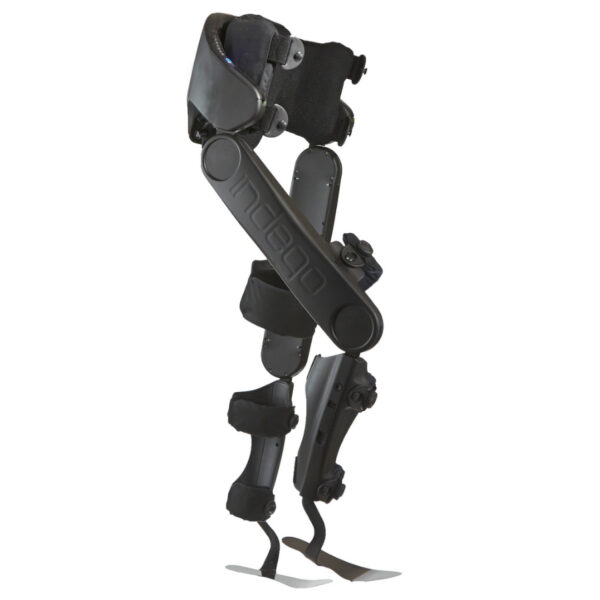
\includegraphics[scale=0.6]{images/background/Indego-via-Parker-Hannifin-Corporation-600x600.jpg}
     \caption[Indigo Exoskeleton]{Indigo Exoskeleton \protect\footnote{\url{https://secureservercdn.net/72.167.25.126/045.a06.myftpupload.com/wp-content/uploads/2016/09/Indego-via-Parker-Hannifin-Corporation-600x600.jpg}}}
     \label{fig:indigo}
 \end{figure}
 
 
 The above exoskeletons all share similar design features. They have powered hips and knees joint to provide supplementary and assistive torque, and the rigid structures provide support. The exoskeletons can be separated into several parts that can be adjusted to fit the person; this helps with the donn/doff timing and difficulty. They aid in rehabilitation by keeping the person active and bones loaded.  
 
The high price makes it difficult to purchase these exoskeletons for research and home and challenging to obtain. Justifying an exoskeleton's purchase without a proven controller is similarly difficult; testing a controller without an exoskeleton is difficult.
 
Designing and building an exoskeleton can is also expensive and time-consuming. Maxon motors can cost \$350+\footnote{\url{https://www.maxongroup.com/maxon/view/product/323772}} each  , Harmonic gearboxes can cost over a \$1000 each and require large lead times for internal reviews \footnote{\url{https://www.harmonicdrive.net/products/rotary-actuators}}. The material cost for structure can cost hundreds to thousands of dollars, including the manufacturing time. In addition, the electrical components must be custom designed to drive the motors and allow for real-time control; this, again, requires proficiency in every field of engineering, from mechanical to computer science. Additionally, a great deal of time would be spent designing, manufacturing, building, and testing the exoskeleton; this would take time and focus from designing new controllers. 
 

 


\subsection{Upper Limb Exoskeletons}
While not the paper's focus,  the development of upper limb rehabilitative exoskeletons should be noted; several robotics systems have been developed for upper limb rehabilitation. These systems are focused on repetitive motion with assistive forces \cite{rehmat2018upper} \cite{krebs2013rehabilitation}, this is applicable to lower limb exoskeletons as well since they need to provide assistive force to help maintain a gait motion. 

One of the early robots developed was the \textbf{MIT-Manus} \cite{krebs2004rehabilitation}. This robot has two DoF's that can move horizontally in the plane, eliminating gravity. A visual feedback system helps the patient engage with the rehabilitation. The robot also provides assistive torque to help the person move through motions.    

\begin{figure}
    \centering
    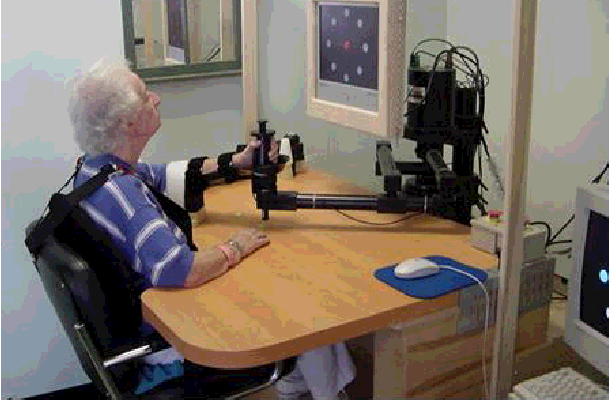
\includegraphics[scale=0.5]{images/background/MIT-MANUS.png}
    \caption[MIT-MANUS]{MIT-MANUS \cite{MIT-Manus}}
    \label{fig:my_label}
\end{figure}


Additionally, the \textbf{UL-EXO7} is a seven DoF robotic arm that provides assistive forces and a full range of motion shown in \autoref{fig:ULEXO7}. This robot, like the MIT-Manus, also is used to play an interactive game. The initial trial has been shown to have functional patient outcomes. 

\begin{figure}
    \centering
    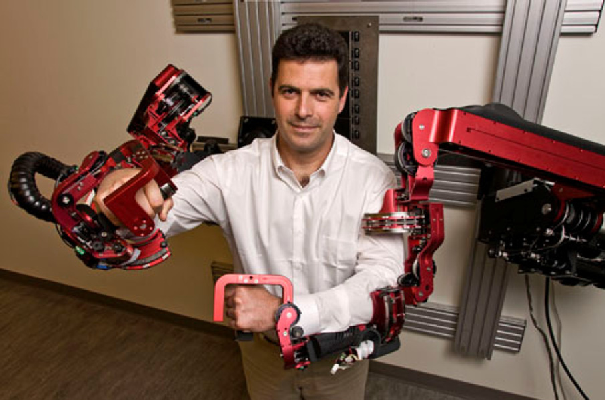
\includegraphics[scale=0.5]{images/background/ULEXO7.png}
    \caption[UL-EXO7]{UL-EXO7 \cite{byl2013chronic}}
    \label{fig:ULEXO7}
\end{figure}


Another rehabilitation arm exoskeleton is the \textbf{T-WREX}. Unlike some of the other systems, the T-WREX is pneumatically powered \cite{TWREX}; this had the advantage of large non-linear forces with low onboard mass. This system has also been shown to have successful rehabilitative outcomes \cite{housman2007arm}.

\section{Functional Electrical Stimulation}
\label{sec:FES}
\subsection{Overview}

Exercise and loading the leg bones can prevent the primary cause of these health side effects. Functional Electrical Stimulation (FES) is a rehabilitation tool used to stimulate muscle activation  \cite{quintero2012preliminary}. There are several benefits of using FES for SCI rehabilitation; clinical outcomes, fitness benefits, and functional gains \cite{hamid2008role}. FES has been used to allow people to stand, walk, and use a cycle\cite{mazzoleni2013fes}. All of which have measurable rehabilitation and health benefits. FES's main complication and limitation is muscle fatigue \cite{karu1995reducing}. Using FES  does not provide any structural support to hold up the person. Mechanical structures can supplement FES to support the patient and add a layer of safety. 

\subsection{Muscle Modeling}
 In \cite{reiner1998patient}, simulation is used to model a patient-driven approach in which the the upper-body effort is used to stimulate leg muscles through Functional Electrical Stimulus (FES) \cite{lynch2008functional} \cite{rushton1997functional}. 
 
 \autoref{eq:activation} shows the muscle stimulation activation where, $a_r(t)$ is the activation based on the stimulation pulse width and $a_f(t)$ is the activation based on the stimulation frequency. The $fit(t)$ term controls the muscle fatigue, which is a result of the calcium dynamics and is shown in \autoref{eq:fatigue}. Here $\beta$ is a scaling term, and $T_{rec}$ and $T_{fat}$ are time constant terms that control how quickly the muscle recover and fatigue. These values are dependent on each of the muscles groups and need to be tuned to the person. \autoref{fig:fagigueExample} shows an example of the effect of fatigue on the activation function; the blue line is the non-fatigued activation, the pulse value is being controlled over time. The graph shows that the orange line is the fatigued activation value and the maximum value is decreased as opposed to the non-fatigued blue line.
 
 
 \begin{equation}
     a &= fit(t) a_r(t) a_f(t)
     \label{eq:activation}
 \end{equation}
 
 \begin{equation}
    \small
    \begin{aligned}
             \frac{dfit}{dt} &= \frac{ (fit_{min} - fit) a \lambda(f) } {T_{fat} } + \frac{ (1 - fit) ( 1- a \lambda(f)) } {T_{rec} } \\
             \lambda(f) &= 1 - \beta + \beta(\frac{f}{100})^2 
    \end{aligned}
     \label{eq:fatigue}
 \end{equation}
 
 

 \begin{figure}
     \centering
     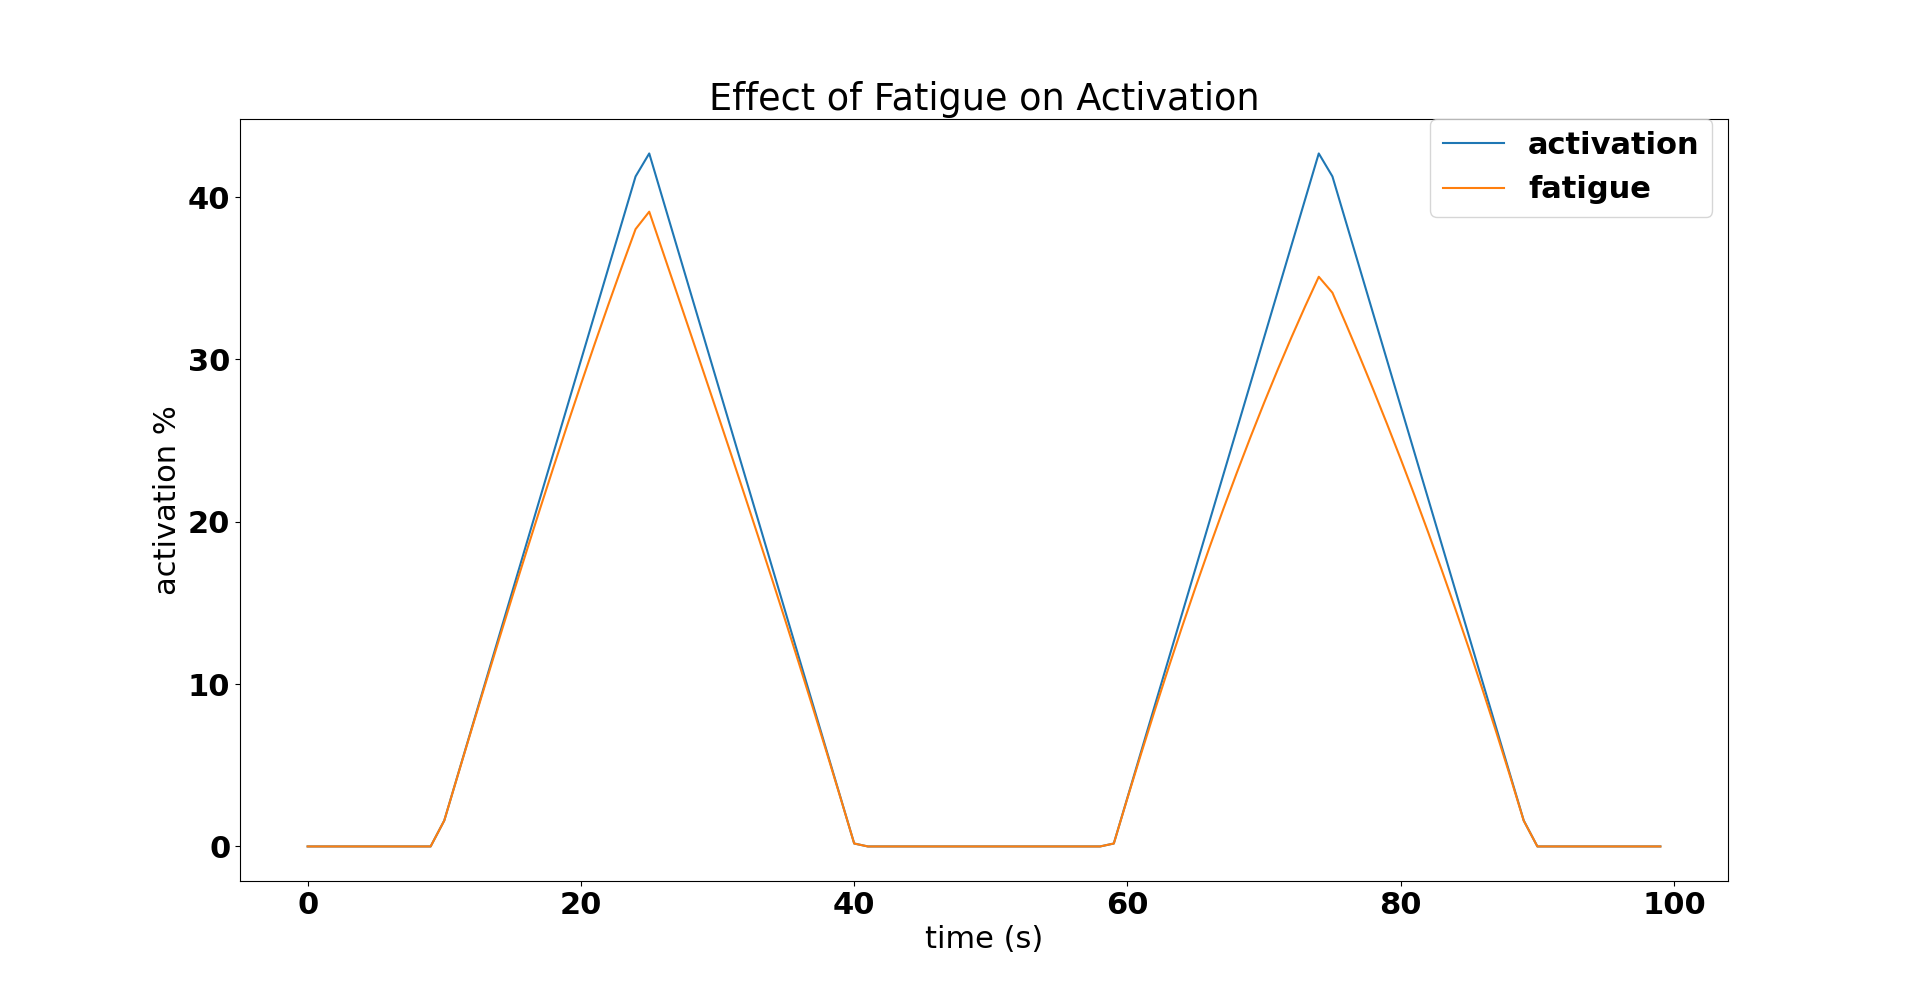
\includegraphics[width=\textwidth]{images/background/activation.png}
     \caption[Fatigue Example]{Fatigue Example}
     \label{fig:fagigueExample}
 \end{figure}
 
 
 The total torque is shown in \autoref{eq:totalMucsle}. The $M_{ela}$ term is calculated from the elastic properties of the muscles. The $M_{vis}$ term is calculated from the viscous properties of the muscles. The $M_{act}$ term is the torque generated from the activation of muscles. These terms are dependent on the moment arms of each of the nine muscles groups in the lower body. These equations are non-linear terms parameterized by the leg's joint angles. The $M_{dyn}$ are the dynamics of the model. 
 
 
 \begin{equation}
     \tau = M_{act} + M_{dyn} + M_{vis} + M_{ela}
     \caption{Total muscle force}
     \label{eq:totalMucsle}
 \end{equation}
 

\subsection{Non-Rehabilitation Exoskeletons}

While rehabilitation exoskeletons are the primary focus of this dissertation, it is essential to note the innovation of exoskeletons designed for strength augmentation and reducing metabolic costs. The application of these exoskeletons ranges from military applications to construction and factory work. These exoskeletons can enhance the user's upper and lower body. Additionally, both soft and rigid exoskeletons have been explored.

In \cite{walsh2006autonomous} Walsh \textit{et. al} presented an under-actuated lower-limb exoskeleton that was able to transmit 90\% of the loads to the ground. Additionally, in \cite{wehner2013lightweight} and \cite{asbeck2013biologically} a soft lower limb exoskeleton was presented and examined, which was able to reduce the metabolic cost during a gait cycle. \autoref{fig:walsh} shows an example of a soft lower limb exoskeleton. These suits use actuated Bowden cables connected to the joints to help pull the joints through the gait cycle. While soft suites have the benefit of being lightweight, they do not provide structural support.  



As discussed above, the \textbf{BLEEX} was designed for military application to increase the load a person was able to carry and reduce the metabolic costs. The research was primarily funded by DARPA\footnote{https://www.darpa.mil/}.  Unlike the suite presented by Walsh, this suite is a rigid system with large powered actuators. \autoref{fig:BLEEX} shows the BLEEX military lower limb exoskeleton.


The \textbf{HAL-5} exoskeleton has both upper and lower body systems. \autoref{fig:HAL5} show the HAL-5 exoskeleton. This system was initially designed as a lower-body assistive device with the upper body; it allows users to increase their load caring capability. This system uses electromyogram (EMG) signals to detect the user's intent and provide assistance \cite{casolo2008active}.


\begin{figure}
     \centering
     \begin{subfigure}{0.5\textwidth}
    \centering
    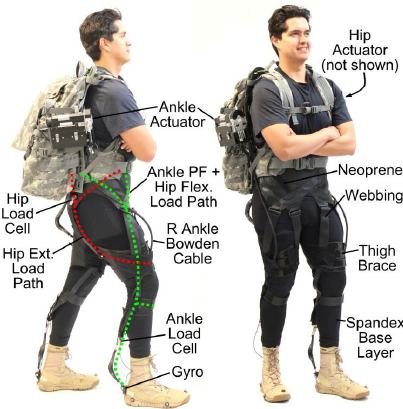
\includegraphics[width=.9\linewidth]{images/background/walsh.png}
    \caption[Walsh soft exoskeleton]{Walsh soft exoskeleton \cite{panizzolo2015evaluation}}
    \label{fig:walsh}
     \end{subfigure}
     \hfill
     \begin{subfigure}{0.3\textwidth}
        \centering
    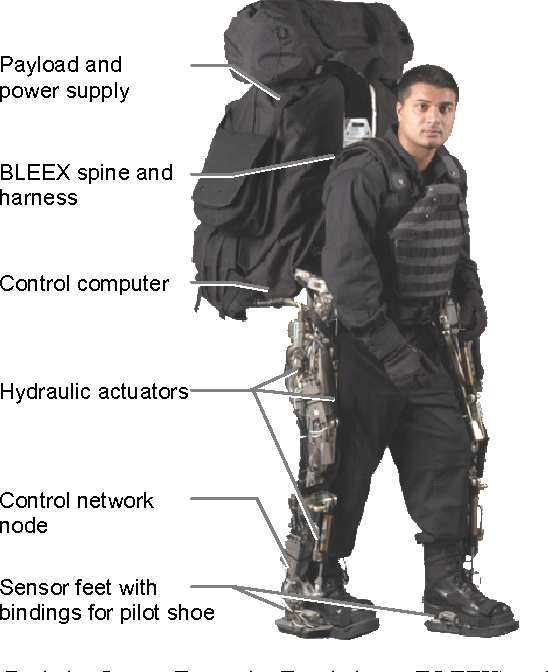
\includegraphics[width=.9\linewidth]{images/background/BLEEX2.png}
    \caption[BLEEX]{BLEEX powered exoskeleton for military applications \cite{kazerooni2006hybrid}}
    \label{fig:BLEEX}
     \end{subfigure}
     \begin{subfigure}{\textwidth}
           \centering
            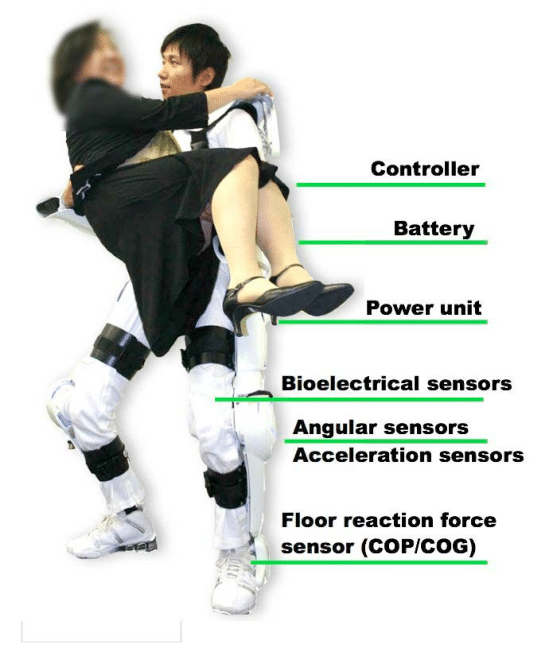
\includegraphics[width=.45\linewidth]{images/background/HAL-5.png}
        \caption[HAL-5]{HAL-5 exoskeleton \cite{sankai2010hal}}
    \label{fig:HAL5}
     \end{subfigure}
        \caption{Enactment Exoskeletons}
        \label{fig:enhanceExos}
\end{figure}

These exoskeletons have similar features as rehabilitation exoskeletons. They both need to be able to detect the user intent and provide assistive torques. However, it should be noted that soft exoskeletons do not provide structural support, which may be necessary if the person cannot support themselves. Additionally, detecting EMG signals maybe be plausible for people with SCI who, due to their injury.

\section{Learning from Demonstrations}
\label{sec:lfd}

\subsection{Introduction}


 Several studies have examined how people walk and climb stairs. Motion capture is one tool used for recording human kinematics and kinetics. In  \cite{chalodhorn2007learning}, Chalodhorn \textit{et. al} used a model-free approach to teach a robot to walk. In  \cite{hu2014online}, Hu \textit{et. al} used quadratic programming to optimize the mapping of the markers to the robot. In both cases, motion capture mapping was used to map from a human to a humanoid robot. This research was limited to direct robot control, and the robot was only able to perform the exact motion of the human.

 In \cite{taskjointmocap}, Hu \textit{et. al} focused on online generations of trajectories. They formulated the control problem as a Quadratic Programming (QP) problem, and the authors used both Cartesian and joint data as the imitation criteria. The formulation as a QP problem allows for inequality and equality constraints for the knee velocity. This formulation resolves the conflicts between the joint space and the Cartesian imitation data. This method is limited to level ground walking. This process did not address abstracting the trajectories for different stair heights; it only addressed level ground walking and fully actuated systems.
 
 Learning from Demonstration allows for complex motions to be learned and reproduced on robotics systems; this enables the desired motion to be taught to the exoskeletons instead of attempting to hand-generate the gait motion needed to accomplish the same goal. This section will show how to use human gait demonstrations to learn and reproduce a gait motion and generate a trajectory to climb stairs.  


\subsection{Overview of methods and applications}
Learning from Demonstration (LfD) is the process of transferring skills to a robot by demonstration. In \cite{siciliano2016springer}  \cite{kormushev2011imitation} \cite{calinon2007teacher} Calinon \textit{et al} outline the process of teaching a robot how to follow a trajectory. There are several steps of LfD: demonstration modality, motion primitives, and encoding methods. There are several steps of the LfD process, as stated below. 

\begin{enumerate}[noitemsep]
    \item Recognition of the task 
    \item Encoding of the motion 
    \item Retrieval of the task 
    \item Reproduction of task 
\end{enumerate} 

There are two primary teaching modalities that teaching methods can be sorted into. These modalities are used to teach a robot to follow a trajectory and to collect data. The first teaching modality is kinesthetic teaching. This modality involves a user moving a robot passively or running an impedance controller through a task while recording the joint positions and torques \cite{Calinon2018}. Researchers have applied kinetic teaching for upper limb robotic systems for industry and human-robot interfaces. While this method is a natural teaching method, it is not well suited for teaching lower limb movement because it would require directly moving a leg through a gait motion. It would be difficult to replicate the leg's motion by the manual moving of a person or robot. 

The second teaching modality is visual observation. In this teaching modality, visual sensors record the desired motions and intentions of a demonstration for mapping onto a robotic system \cite{CalinonLee19}. In visual observation, mocap is the standard method. The marker system allows for precise tracking of points on a person with millimeter accuracy \cite{ott2008motion}. This method has broad adaptation capabilities and high accuracy for gait data collection \cite{ViconGaiting}.

Dynamic Motion Primitive (DMP) is a method of breaking down demonstrations into their fundamental building blocks; it is a popular form of motion primitive \cite{ijspeert2013dynamical}. Motion primitives aim to encode trajectories into building blocks that can be rearranged and manipulated.  DMP works by creating a stable underlying model and generating a forcing function to drive the system.  

There are several LfD methods for learning trajectories and building models based on the data from the two teaching modalities, including Locally Weighted Regression (LWR), Hidden Markov Models (HMM), and Gaussian Mixed Regression (GMR). They are all methods of encoding motion into basis functions for learning and reproduction. These methods are similar, but each method contains its unique pros and cons. LWR is the simplest method, with HMM and GMR being extensions of this method. HMM and GMR places the radial basis functions (RBF) on the trajectory more effectively.  

HMM combines temporal scaling and transition probabilities through a double stochastic process \cite{calinon2007learning}. HMM has built-in temporal scaling, meaning that it can deal with demonstrations that are not aligned. The double stochastic process makes it challenging to retrieve smooth and continuous trajectories; this makes it unsuitable for teaching exoskeleton trajectories, as stated by Calinon \textit{et. al}. The GMM method produces smooth and continuous trajectories, making it better suited for producing trajectories for exoskeletons. 

The GMR method uses GMM to provide a more comprehensive approach to the RBF placement and allows for the encoding of multiple trajectories \cite{calinon2013compliant}. GMM is similar to K-means; however, it uses the Expectation-Maximization (EM) algorithm to find the optimal placement of the RBF on the data set. GMR is used to regress the RBFs to find an underlining model. The demonstrations require temporal alignment before being encoded. Dynamic Time Warping temporally aligns two demonstrations (DTW). The DTW algorithm attempts to minimize the distance between two trajectories by drawing lines between the two curves \cite{muller2007dynamic} \cite{JSSv031i07}. 
 GMR is computationally fast and produces smooth and continuous trajectories. The benefits of using GMR are the following \cite{Calinon}: 


\begin{enumerate}[noitemsep]
    \item Allows encoding of local correlation between motion variables
    \item Provides a principled approach to estimate the parameters of the RBF 
    \item Reduce the number of RBF   
    \item Online estimation of the DMP parameters and model selection   
\end{enumerate}  

There are four steps for building the imitation model listed below. \autoref{fig:demostation} illustrates the workflow for training and reproduction.

\begin{enumerate}[noitemsep]
    \item Collection of gait data
    \item Encoding of motion into RBF
    \item Learning of regression function
    \item Reproduction, and manipulation of the trajectories
\end{enumerate}


\begin{figure} 
    \centering 
    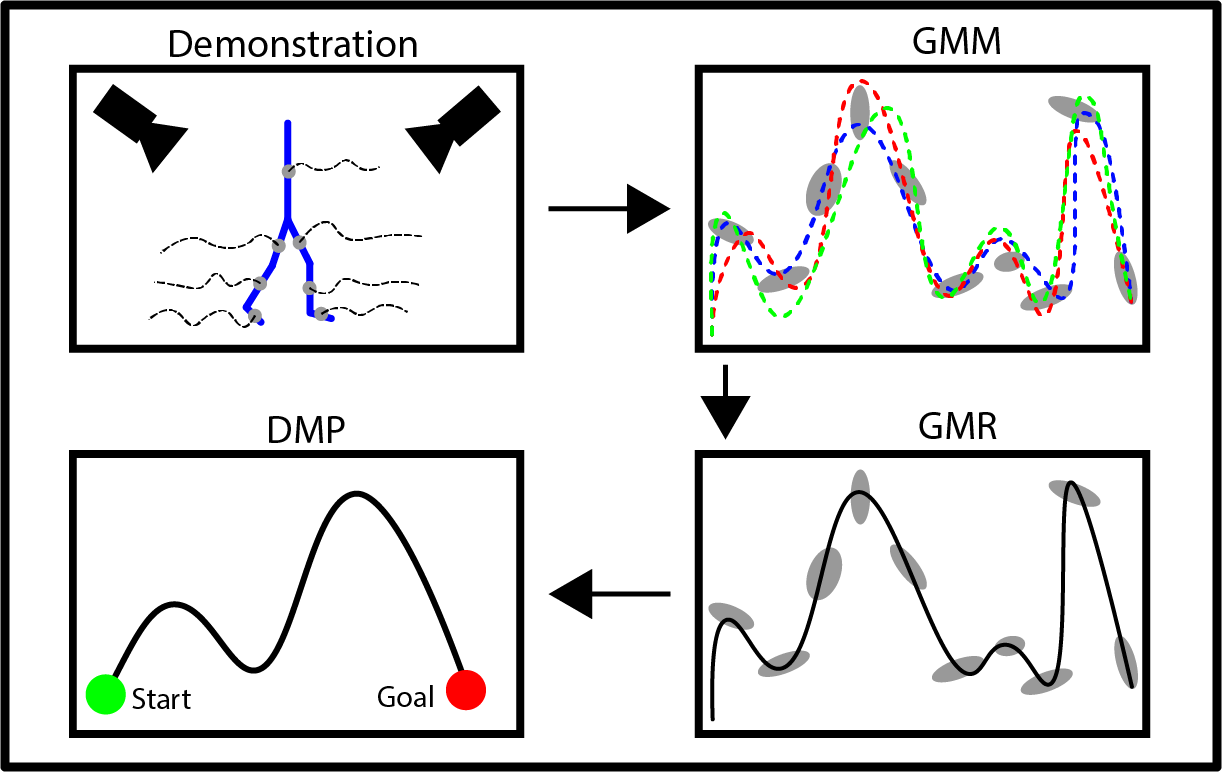
\includegraphics[scale=0.25]{images/background/demo_figure.png} 
    \caption[Learning Process]{Order of operations of the learning process. The data is collected, the demos are encoded and aligned with DTW, the model is retrieved, then the model is reproduced.} 
    \label{fig:demostation} 
\end{figure} 


In the classical formulation of DMPs, the model places radial basis functions (RBF) along the single demonstration to pull the system towards the goal. GMR/GMM replaces this method with a methodical placement of the RBFs and multiple demonstrations to train the model. DMPs are considered one of the gold standards of learning and replicating human motion \cite{nakanishi2004learning}.


To compare and encode the demonstrations, they have to be the same length. When recording live motion data, the demonstrations of the same task will be of different lengths depending on how fast the subject moves; this will create demonstrations that are similar in motion but are not temporally aligned. These demonstrations could be aligned by re-sampling the trajectories to be the same length. However, there is no guarantee that the features of the trajectories will align after they are re-sampled. This problem can be resolved by using Dynamic Time Wrapping, which provides a principled approach to align demonstrations by finding the minimum distance between each point of the demonstrations \cite{JSSv031i07}. DTW ensured that similar parts of the trajectories aligned with each other. 

\subsection{Mathematics of Learning}
 

 \autoref{eq:DTW} shows the equation for DTW; it maps demo 2 onto demo 1. Here, $\delta (P, T)$ is defined as the Manhattan distance function. $P$ and $T$ are demo 1 and demo 2, respectively. This method maps $P$ onto $T$ . Here, $w_k$ is the cost at index $(i,j)$, and $k$ is the time frame. \autoref{fig:DTW_example} illustrates how DTW functions. Here two $cosine$ functions of different lengths are aligned. The cost matrix path shows that the demonstrations are aligned. The path is the minimum cost through the matrix. The illustration shows one of the primary problems with DTW; the time-wrapped trajectory (green line) has sharp bends in the line, it does not produce smooth trajectories. This problem can be solved by fitting a polynomial to the time-wrapped trajectory shown as the red line.  
 
 \begin{figure}
     \centering
     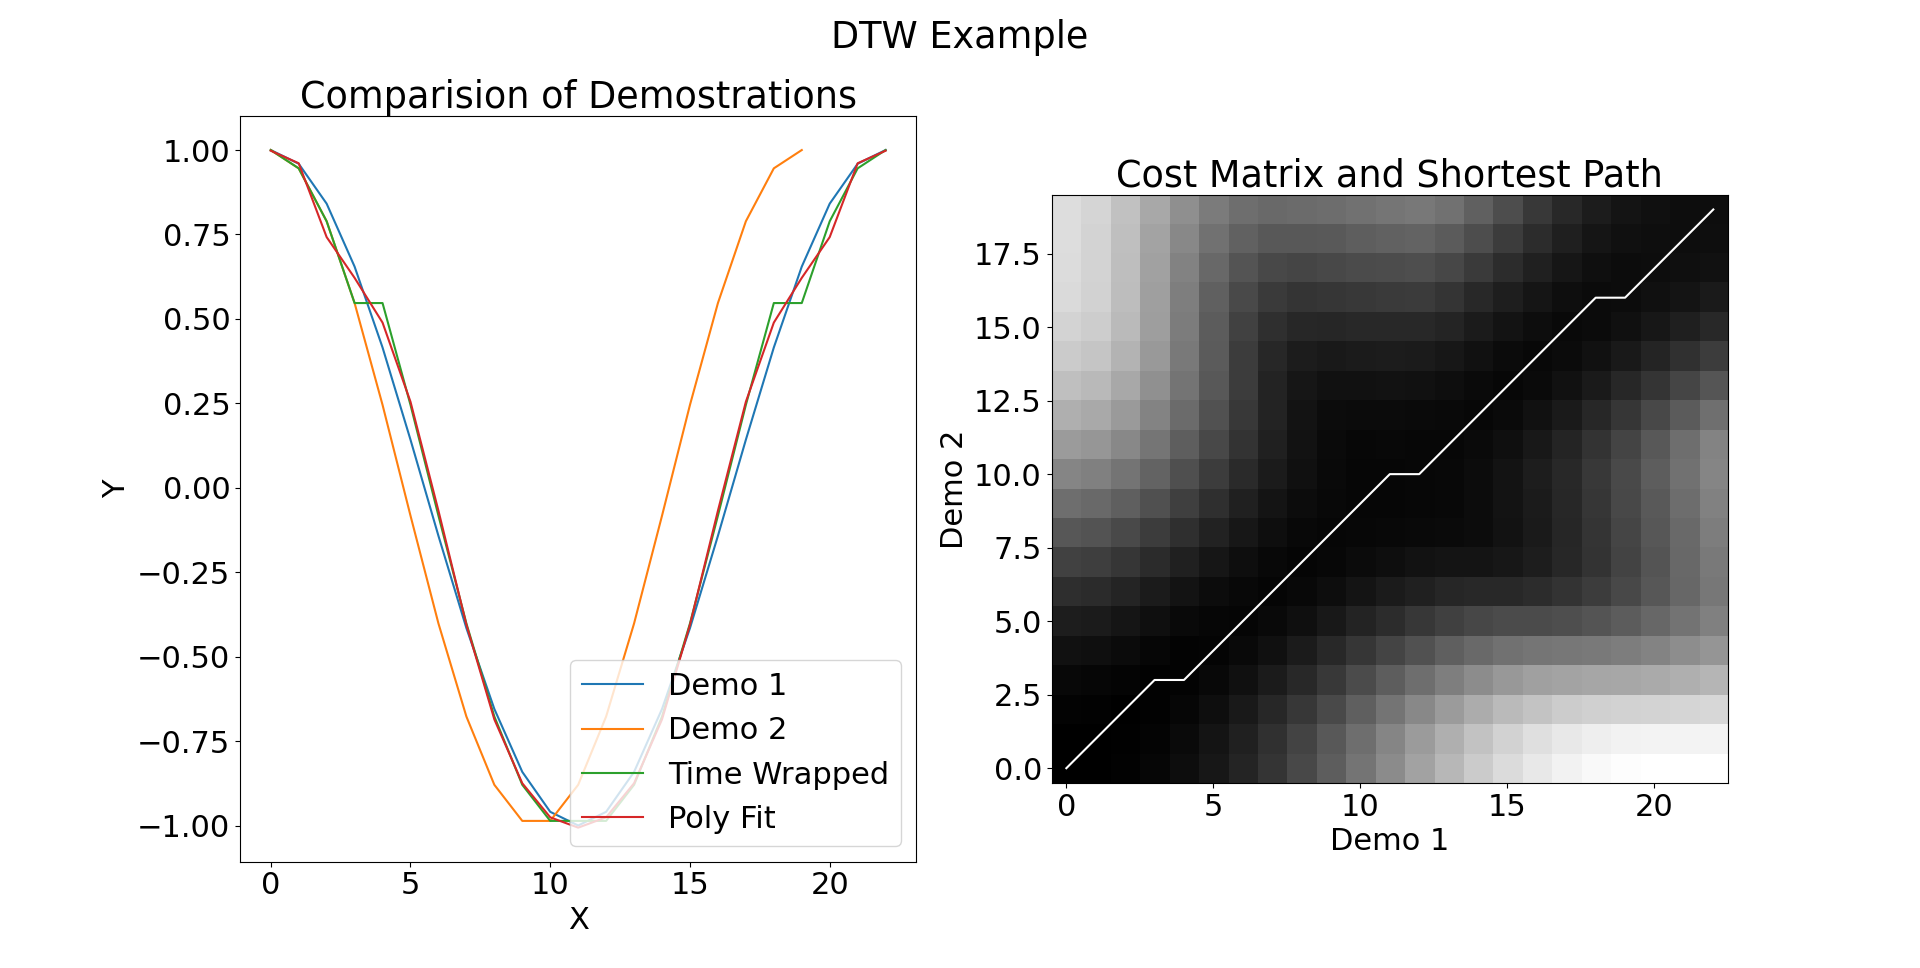
\includegraphics[scale=0.3]{images/background/DTW_example.png}
     \caption[DTW Example]{Two demos being aligned using DTW and a smoothed trajectory. Blue line: demo 1. Orange line: demo 2. Green line: aligned trajectory. Red line: Poly Fit The cost map shows the distance between the points. }
     \label{fig:DTW_example}
 \end{figure}

\begin{equation} 
    \begin{aligned} 
         \delta (P,T) &= | p_i - t_j| & \text{Distance function} \\ 
        DTW(P,T) &= min \Bigg[ \sum_{k=1}^{K} \delta (w_k) \Bigg] & \text{Minimum path} 
    \end{aligned} 
    \label{eq:DTW} 
\end{equation} 


DMPs work by developing an underline stable motion model and adding a forcing function to drive the system along the trajectory. \autoref{eq:DMP_Model} control how the system moves along the trajectory, where $\alpha_y$ and $\beta_y$ are gains and $y$ is the system state. This system acts as a PD controller. The forcing function $f$ drives the systems by placing RBF along the trajectory and attracting the system to the points. The forcing functions is built using \autoref{eq:DMP_force}. Here $w_i$ is the weighting on the basis function $\psi_i$ defined by the Gaussian's centered at $c_i$ where the $h_i$ is the variance. As the system moves along the trajectory, the Gaussians are activated and pull the system. DMPs are limited to the use of a single demonstration for training.  

\begin{equation}
    \Ddot{y} = \alpha_y ( \beta_y ( g - y) -\Dot{y}) + f
    \caption{DMP model}
    \label{eq:DMP_Model}
\end{equation}


\begin{equation}
 \begin{split}
    \Dot{x} &= -\alpha_x x \\
    f(x,g) &= \frac{\sum_i^N \psi_i w_i}{\sum_i^N \psi_i}x(g-y_0)\\
    \psi &= \exp( -h_i (x -c_i)^2)
 \end{split}
    \caption{DMP model}
    \label{eq:DMP_force}
\end{equation}

The GMM method uses the EM algorithm that iteratively updates the probabilities of the points.  \autoref{eq:Estep} and \autoref{eq:Mstep} show the two steps in the EM algorithm. In these equations, $X$ is the point vector, $h$ is the posture probability, $\pi$ is the weighting coefficient for each point, $\mu$ is the mean, and $ \Sigma $ is the covariance.  K-means is used to find the initial guess of the $\mu$ and $\Sigma$ parameters for the EM algorithm with the value of $\pi$  initialized randomly. 

E(xpectation)-step:


\begin{equation} 
    \centering
     h_{t,i} = \frac{\pi_i \prod_{j=1}^{P} \mathcal{N}(X_t^j | \mu_i^j , \Sigma_i^j )}{ \sum_k^K \pi_k \prod_{j=1}^{P} \mathcal{N}(X_t^j | \mu_k^j , \Sigma_k^j ) } 
     \label{eq:Estep} 
\end{equation}{} 

M(aximization)-step: 
\begin{equation} 
\begin{aligned} 
    \pi_i &\leftarrow \frac{\sum_t^N h_{t,i}}{N} \\ 
    \mu_i^j &\leftarrow \frac{\sum_t^N h_{t,i} X_t^j}{\sum_t^N h_{t,i}} \\ 
    \Sigma_i^j &\leftarrow \frac{\sum_t^N h_{t,i} ( X_t^j - \mu_i^j)  ( X_t^j - \mu_i^j)^T   }{\sum_t^N h_{t,i}}  
\end{aligned} 
\label{eq:Mstep} 
\end{equation} 



TPGMM is similar to the Gaussian mixed model (GMM); the difference between TPGMM and GMM is that TPGMM models the importance of a task in the frame rather than the constant Gaussian ($\mu_$, $\Sigma_i$). The model is defined by $ \{ \pi_i \{ \mu_i^j , \Sigma^j \} _{j=1}^P \}$, $\pi_i$ is the mixing coefficient, $\mu$, is the mean, and $\Sigma$ is the covariance matrix of the Gaussian.
 The EM equations are altered to handle the importance of a task in the frame. The altered  E-step and M-step are shown in \autoref{eq:EstepTPGMM} and \autoref{eq:MstepTPGMM}.

E(xpected)-Step:
\begin{equation}
    \gamma_{n,i} = \frac{\pi_i \prod_{j=1}^{P} \mathcal{N}( X_n^j | \mu_i^j, \Sigma_i^j)  }{   \sum_{k=1}^{K} \pi_k \prod_{j=1}^{P} \mathcal{N}( X_n^j | \mu_i^j, \Sigma_i^j)}
    \label{eq:EstepTPGMM}
\end{equation}

 M(aximization)-Step:
 
\begin{equation} 
\begin{aligned} 
    \pi_i &= \frac{\sum_t^N \gamma_{t,i}}{N} \\ 
    \mu_i^j &= \frac{\sum_t^N \gamma_{t,i} X_t^j}{\sum_t^N \gamma_{t,i}} \\ 
    \Sigma_i^j &= \frac{\sum_t^N \gamma_{t,i} ( X_t^j - \mu_i^j)  ( X_t^j - \mu_i^j)^T   }{\sum_t^N \gamma_{t,i}}  
\end{aligned} 
\label{eq:MstepTPGMM} 
\end{equation} 


The covariance matrix is square and of size $N+1$, where $N$ is the number of trajectories to be trained, where the first element is the time relationship. This is illustrated in \autoref{fig:cov_mat}, the covariance matrix used to calculate the Gaussian are $2x2$ sub-matrix of the larger matrix. They are constructed by taking the time element with the current training model $T$, for all training trajectories $1..N$. The number of matrix $K$ is detriment by the number of bins set. The sub-covariance matrix determines the shape and size of the gaussian ($\Sigma$), where the mean  ($\mu$) determines the location along the trajectory. 


\begin{figure}
    \centering
    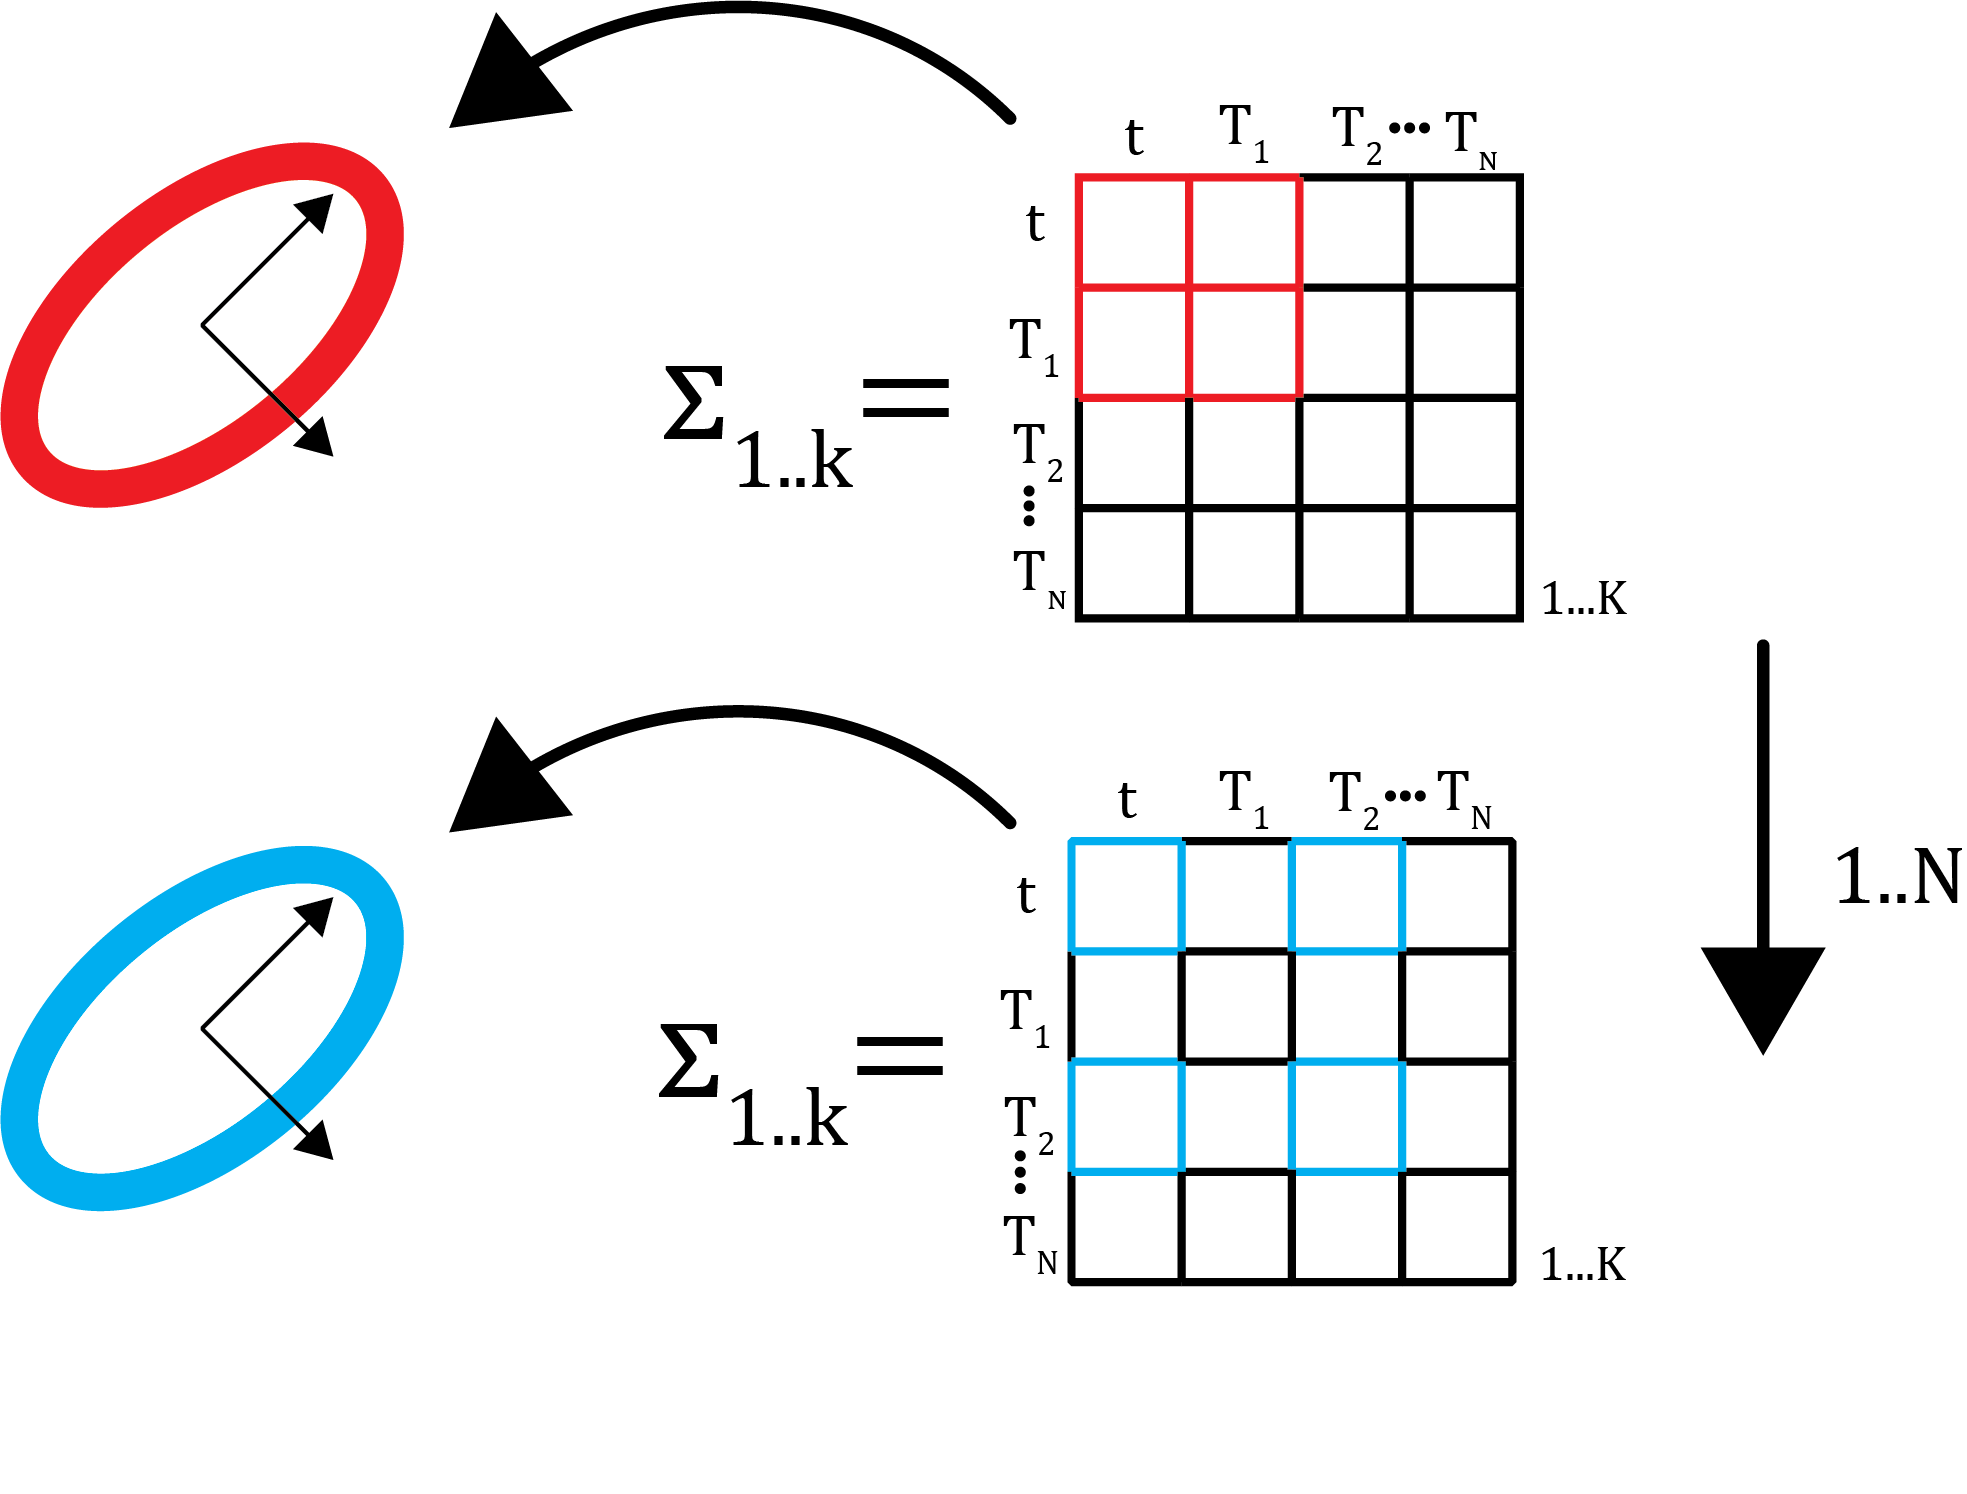
\includegraphics{images/background/cov_matrix.png}
    \caption[Covariance Matrix Illustration]{Using the covariance matrix ($\Sigma$) to calculate the gussian for each of the trajectories}
    \label{fig:cov_mat}
\end{figure}



Each of the demonstrations $d \in \{1...D \}$ is a vector of time-sequenced data points and is of $T_d$ size. This results in a data structure of size $\sum_{d=1}^D T_d$. The length of each of the $T_i$ vectors will be different for each demonstration; this results from the subjects' stride speeds. 

The task parameters are represented as a coordinate system $P$ defined at each time step n defined by $\{ b_{n,j}, A_{n_j} \}^{P}_{j=1}$. The $b$ vector is a set of basis vectors from the origin with the transformation matrix $A$. This formulation allows for trajectories to be transformed into any frame using \autoref{eq:transform}. $\xi$ is the vector of the data points.

\begin{equation}
    X_t^j = A^{-1}_{t,j} ( \xi_t - b_{t,j})
    \label{eq:transform}
\end{equation}



 \autoref{eq:GMR_Prop} calculates the likelihood, and \autoref{eq:GMR_mu} calculates the covariance and mean. Where $\xi_$ is a multidimensional array, $\mu_i^o$, and $\Sigma_t^o$ are vectors of the output mean, and covariance, $\mu_i^I$, and $\Sigma_t^I$ are vectors of the input mean and covariance. 
GMR models the regression function from the joint probabilities in the form of GMM. 

\begin{equation} 
     P(\xi_t^O | \xi_t^I ) \sim \sum_i^K h_i(\xi_t^I) \mathcal{N}( \hat{\mu_i^o}, \hat{\Sigma_t^o}) 
     \label{eq:GMR_Prop} 
\end{equation} 

where, 

\begin{equation} 
    \begin{aligned} 
      \hat{\mu_i^o} &= \mu_i^o + \Sigma_i^{OI}\Sigma_i^{I-1}(\xi_t^I - \mu_i^I)\\ 
      \hat{\Sigma_i^O} &= \Sigma_i^O - \Sigma_i^{OI}\Sigma_i^{I-1} \Sigma^{IO}_i \\ 
       h_{i} &= \frac{\pi_i \mathcal{N}(\xi_t^I | \mu_i^j , \Sigma_i^j )}{ \sum_k^K \pi_k \mathcal{N}(\xi_t^I | \mu_k^j , \Sigma_k^j ) }   
    \end{aligned} 
    \label{eq:GMR_mu} 
\end{equation} 

The number of bins $ K $ used in TPGMM are found using the Bayesian Information Criterion (BIC); if too few bins are used, the model will be poorly fit; if too many are used, it will over-fit the demonstrations. BIC is a method to overcome this limitation and find the optimal number of bins \cite{calinon2007learning}. \autoref{eq:BIC} calculates the BIC score; it is a trade-off between optimizing the likelihood and minimizing the number of states to encode.  $\mathcal{L}$ is the log-likelihood, $ N $ is the number of mixture models, $ K $ is the number of components, and $ D $ is the dimension of the data points. 


\begin{equation} 
    S_{BIC} = -\mathcal{L} + \frac{log(N)(K(D+1)(D+2)-2)}{4}  
    \label{eq:BIC} 
\end{equation} 


A reproduction model's accuracy is measured by calculating the imitation cost; this is essentially a root mean squared algorithm that measures how well the model follows the demonstrations \cite{metric}. \autoref{eq:metric} shows the equation used to calculate the goodness of fit. In this equation, $d$ is the demo, $m$ is each of the demos, $t$ is the time, and $x$ is the trained model. 

\begin{equation}
    C = \frac{1}{MT} \sum_m^M{\sum_t^T{ || d^m_t - x_t||}}
    \label{eq:metric}
\end{equation}


 \begin{figure}
     \centering
     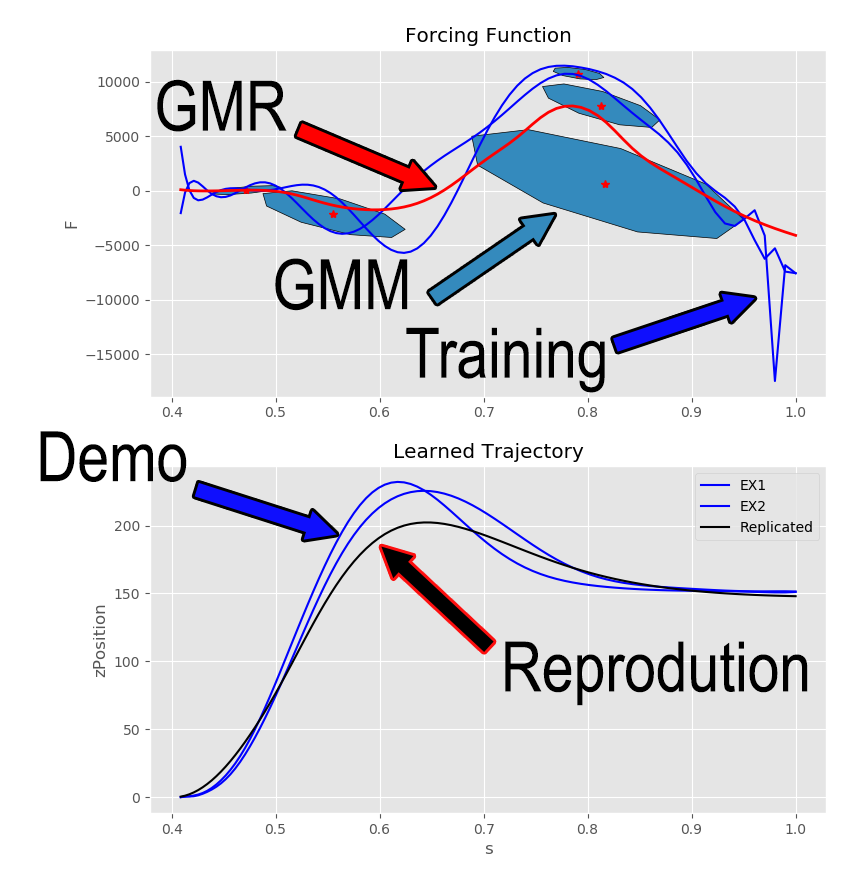
\includegraphics[scale=0.42]{images/background/GMM_reproduction.png}
     \caption[Simple Reproduction Example]{Demonstration of how LfD reproduces trajectories with the labeled components. This Model was generated using two demonstrations collected from stair climbing data. }
     \label{fig:SimpleGMMExample}
 \end{figure}

\subsection{Applications of LfD}
\label{sec:applfd}
Learning from Demonstration has been used to teach robots a variety of complicated tasks and motions. In \cite{mulling2013learning}, they used motion primitives to train a robot to play table tennis. Similarly, it was used to teach a robot to a robot reach and grasp various objects such as balls and chess pieces \cite{calinon2007active}  \cite{hersch2008dynamical}. It has also been used to learn handwriting \cite{kulvicius2011joining}. All of the thesis tasks share a biological movement has their training set. The robots need to replicate a complex human-like motion that would otherwise be difficult to hand code. The learning from demonstration framework allows for a human demonstration to be collected and encoded onto the robotic system to teach the required movement.  

Learning from Demonstration has not yet been explored to the fullest for imitating lower body motion. Using human demonstration and motion capture offers several advantages over other methods. The high accuracy and rich data set offer the ability to study both the inverse and forward kinematics of the person's legs and trunk, which allows for learning the joint angles or foot position; this is used to train the exoskeleton for different activities of daily living including walking and stair climbing. The difficulty arises in the mapping of the joint motion and how to learn the motion. Using the joint angle ignores the foot placement, while using the foot's location disregards the joint angles. Both of which are important when trying to maintain balance and natural joint motion. In addition, a person's joints cannot move through the desired motion as an arm, so external motion must be mapped onto the person who will have different leg lengths. 



% Stair climbing is a non-linear motion. Ascending stairs require one foot to remain on the ground while the other foot swings through a trajectory\cite{hicks2012temporal}. Several studies have examined how people climb upstairs. Motion capture is one tool that can be used for recording human kinematics and kinetics. In  \cite{chalodhorn2007learning}, Chalodhorn \textit{et. al} used a model-free approach to teach a robot to walk. In  \cite{hu2014online}, Hu \textit{et. al} used quadratic programming to optimize the mapping of the markers to the robot. In both cases, the motion capture mapping was mapped from a human to a humanoid robot. This research was limited to direct robot control, and the robot was only able to perform the exact motion of the human.

%  In \cite{taskjointmocap}, Hu \textit{et. al} focused on online generations of trajectories. They formulated the control problem as a Quadratic Programming (QP) problem, and the authors used both Cartesian and joint data as the imitation criteria. The formulation as a QP problem allows for inequality and equality constraints for the knee velocity. This formulation resolves the conflicts between the joint space and the Cartesian imitation data. This method is limited to level ground walking. This process did not address abstracting the trajectories for different stair heights; it only addresses level ground walking and fully actuated systems.
 
%  Using the foot's position to train an exoskeleton to replicate the stair climbing motion allows for the reproduction of natural biological movement and the abstraction of the stair height. The existing methods are improved using human motion to define the trajectories instead of random motion generation and can be used to move the foot to different stair heights. 
 
%  This method, however, offers several challenges. The first challenge is how to find the joint angles from the foot position for various people. While the Cartesian position of the foot is controlled, the only actuation is in the joints. The joint angles need to be found for people of various heights; this complicates the process because it adds a layer of abstraction.  Another challenge is dealing with the collision with the environment. While controlling the foot, it should not collide with an object; this problem must be tackled for robotic manipulators but not for controlling lower limb robotic systems. Using learning from demonstration to control lower limb robotic platforms has the complexity necessary for varying joint lengths and collisions with the environment. Both of these problems remain unexplored and need further research.  

\section{Exoskeleton Simulations}
Physics-based and graphical simulation is a crucial aspect of exoskeleton development. It allows the development of multiple control algorithms for the exoskeleton without the difficulties of experimentally testing the exoskeleton on a person. Simulation allows the system to be modeled, controlled, and tested before the implementation in experimental environments. It can be a complicated method, but it is essential to develop the controllers \cite{ZLAJPAH2008879}.   

Sit-to-stand motion is one of the many movements modeled in simulation to model dynamics and test control algorithms. In \cite{reiner1998patient}, simulation is used to model a patient-driven approach in which the the upper-body effort is used to stimulate leg muscles through Functional Electrical Stimulus (FES) \cite{lynch2008functional} \cite{rushton1997functional}. Simulink/Matlab designed a tracking algorithm to model the upper body of the human. The PID controller implemented in Matlab/Simulink \footnote{https://www.mathworks.com/products/matlab.html} controlled the orientation of the human's torso. 

Yan \textit{et. al} combined the Automated Dynamic Analysis of Mechanical Systems \footnote{https://www.mscsoftware.com/product/adams} (ADAMS) and Matlab/Simulink to compare the trajectory of an exoskeleton controlled with a PID controller to their developed sliding mode control algorithm \cite{Yan_2017}. ADAMS is the simulation environment for the physical model, while MATLAB calculates the control algorithm. ADAMS was also used by Copilusi \textit{et. al} to perform dynamic analysis of a light-weight lower-extremity exoskeleton, where simulation results presented ample performance for walking rehabilitation  \cite{copilusi2014}. ADAMS also performed the numerical simulation \cite{geonea2017design} of the lower-extremity exoskeleton and compared the experimental walking of healthy subjects. 

While all these approaches have different objectives, they all successfully use simulation to model and develop controllers for their systems;   this shows the versatility and capability of using simulation for exoskeleton development. 

\chapter{Collection and Analysis of Human Gait Data}
\label{chap:gaitdata}
\section{Introduction}

Marker-based motion capture systems(mocap) are popular methods of collecting biomechanical data. The body's movement can be tracked by placing markers on various locations on a person's body. These systems produce significant data, including marker positions, joint angles, and rigid body orientation. Additional sensors, such as Electromyography sensors (EMGs), force plates, and inertial measurement units (IMUs), can be added to measure muscle activity and joint torques. Marker-based trackers work by using several 2D cameras to track the 3D position of retro-reflective markers.  

Biomechanists and engineers use this data for kinematics, dynamics, and kinetics of human motion analysis, and to learn motion primitives of human motion \cite{10.7717/peerj.918}. It has been used for the assessment of orthosis \cite{kobetic2009development},  to analyze gait motion for people with lower-limb impairments \cite{lauer2005application} \cite{hicks2011lower}  \cite{cutler2015using} , and to learn and replicate human motion \cite{ott2008motion} \cite{chalodhorn2007learning}. 

The human leg is built with three joints; a hip, a knee and an ankle. The hip can be modeled as a ball and socket joint allowing for abduction/adduction, and transverse external/internal rotation \cite{faptakinesiology}. The knee is not a simple hinge joint, and the tibia extends during flexion/extension rotation. It allows slight abduction/adduction and internal/external rotation. The knee is also responsible for taking loads during a gait cycle \cite{kuo2007six}. The ankle joint is a synovial joint that helps absorb loads during a gait cycle. These joints are essential for understanding the gait cycle.


\section{Motion Capture Trials}

One of the Motion Caption Trial's goals is to collect enough data to mimic the motion of a healthy gait.  Despite how widely studied and researched the gait cycle and the numerous gait trials conducted, there is very little open-source raw data available, the most popular is the Winter $\it{et. al}$ database \cite{winter1991biomechanics}, yet this library only contains a few subjects. There are other gait data libraries available, but small and have additional restrictions for use. There is a need for additional data to be released for public use. The more data available, the better it helps to train robotics systems and develop exoskeletons and orthosis \cite{moore2015elaborate}. Additional gait and human motion data were collected and released open-source in Github \footnote{https://github.com/WPI-AIM/AIM\_GaitData} to solve this problem. The gait database comprises measurements of how gait varies from person to person when walking across the floor several times and climbing stairs of varying heights. 


\subsection{System setup}
\label{sec:setup}
The Vicon\footnote{Vicon Motion Systems Ltd, Oxford, UK}  Vantage V5 running at $100Hz$ was used to record the locomotion of a person. The system consisted of 10 cameras to track the position of the reflective markers. The makers were placed according to the plug-in gait lower limb template. Two AMTI \footnote{https://www.amti.biz/index.aspx} force plates were placed in the ground to record the joint dynamics. The force plates were synced to the Vicon through the Lock+ box \footnote{https://www.vicon.com/hardware/devices/lock/} running at $1000Hz$. \autoref{fig:markers} shows the placement of the markers on the legs of the subject. 



\begin{figure}
\centering 
\begin{subfigure}{0.4\linewidth} 
  \centering 
  \includegraphics[scale=0.05,frame]{images/gait_data/marker_side_cap.png} 
  \caption[Side Marker Placement]{Side few of the markers} 
  \label{fig:markers_side} 
\end{subfigure} 
%
\begin{subfigure}{0.4\linewidth} 
  \centering 
  \includegraphics[scale=0.05,frame ]{images/gait_data/front_markers_cap.png} 
  \caption[Front Marker Placement]{Front view of the markers} 
  \label{fig:markers_front} 
\end{subfigure} 
\caption[Marker Placement]{The markers were placed according to the plugin marker template. Additional rigid body plates were placed on the subjects' thighs, shanks, feet and back} 
\label{fig:markers} 

\end{figure} 

% \begin{figure}
%     \centering
%     \includegraphics{images/gait_data/marker_side_coor.png}
%     \caption{Marker position for gait collection}
%     \label{fig:gaitmarkerlayout}
% \end{figure}

Eleven able-bodied subjects participated in the study (5F, 6M). The Institutional Review Board of Worcester Polytechnic Institute approved the study, and each subject gave written consent. The data was anonymous, so the subjects could not be identified. \autoref{tab:subjects} holds the metadata of the subjects. All the data was saved in an ASCII format file. The custom open-source software package parses the data (\autoref{chap:software}).

\begin{table}[h!]
\centering
 \begin{tabular}{|c c c c c|} 
 \hline 
 \multicolumn{5}{|c|}{Subjects} \\
 \hline
 ID & Mass ($Kg$) &  Height($m$)  & Age($yr$)  & Gender \\ [0.5ex] 
 \hline\hline
 0 & 59 & 1.6 & 20 & F \\
 \hline
 1 & 62 & 1.7 & 20 & F \\ 
 \hline
 2 & 86 & 1.9 & 44 & F \\
 \hline
 3 & 64 & 1.8 & 20 & M \\ 
 \hline
 4 & 50 & 1.5 & 20 & F \\
 \hline
 5 & 96 & 1.6 &  19 & F\\
 \hline
 6 & 77 & 1.8 & 22 & M \\
 \hline
 7 & 78 & 1.8 & 22 & M \\
 \hline
 8 & 95 & 1.7 & 33 & M \\
 \hline
 9 & 85 & 1.8 & 21 & M \\
 \hline
 10 & 69 & 1.7 & 22 & M \\[1ex] 
 \hline
\end{tabular}
\caption[Subject Meta Data Table]{The Subject's Meta Data Record at Time of the Trial.}
\label{tab:subjects}
\end{table}



 In the first task, the subjects walked approximately 3$m$ at their own pace and stride length \cite{peters2014concurrent}. The subjects were allowed to choose their leading leg. The subject walked across the floor three times to ensure that good data was collected. 

 In the second task, the subjects walked forward approximately 2$m$ and climbed three steps at their own pace. Markers were placed on each step of the staircase and on the floor to record their positions. The subjects approached the staircase, paused, and climbed the stairs with their leading leg. Each subject was allowed to climb at their own pace. Each subject repeated the action three times for each of the four different stairs of different heights, stair heights given in \autoref{tab:stairs}. The repetition of each subject ensured that a good sample trial with no marker occlusion was collected.   
 \begin{figure}[h]
    \centering 
    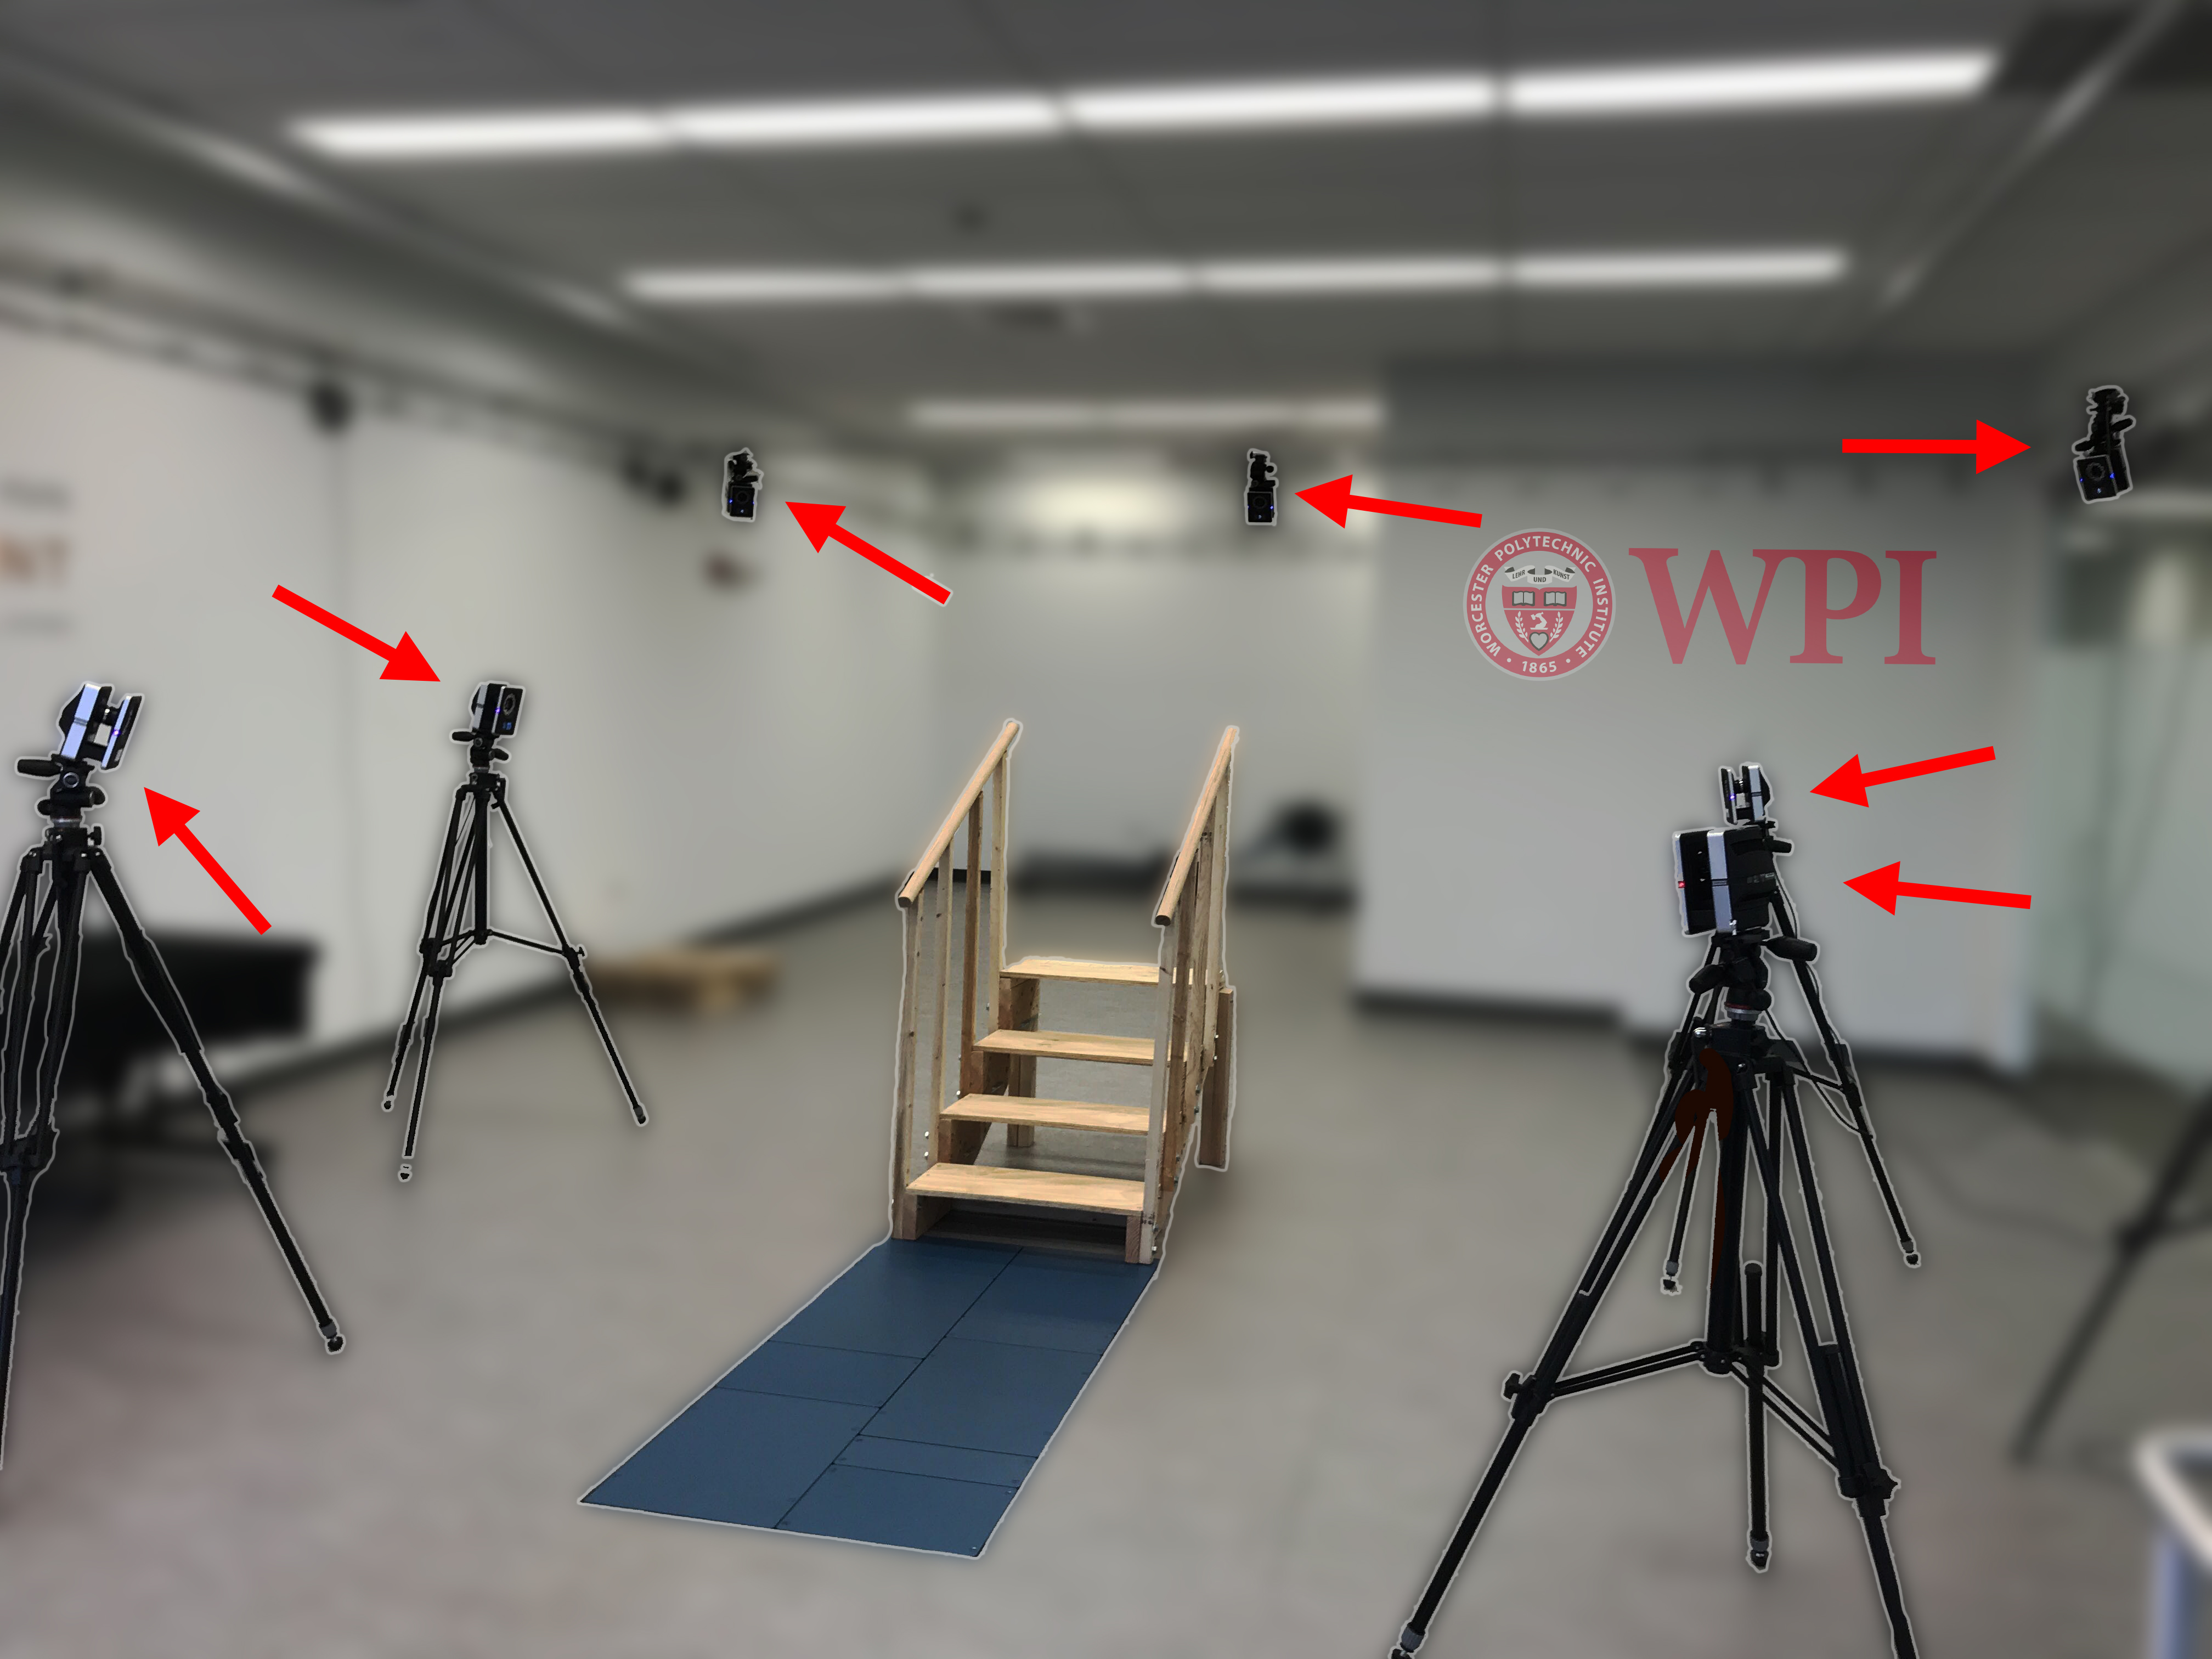
\includegraphics[scale=0.1,frame]{images/gait_data/stairs_EDIT.jpg}
    \caption[Motion Capture Area]{Motion capture area with custom staircases. The stairs had sliding planes to adjust the heights. Seven of the camera are shown and indicated with the green arrows and additional three camera are located off the image.  }
    \label{fig:mocap} 
\end{figure} 
 
\begin{table}[h!]
\centering
\large
 \begin{tabular}{||c c ||} 
 \hline
 Config & stair height (inch) \\ [0.5ex] 
 \hline\hline
 0 & 5.25  \\ 
 \hline
 1 & 6.0  \\
 \hline
 2 & 6.75  \\
 \hline
 3 & 7.5 \\
 \hline
\end{tabular}
\caption{Stair Height Configuration}
\label{tab:stairs}
\end{table}



\section{Analysis of Human Gait}

The goal of collecting the human motion data was to build a model for replicating the gait cycle to allow the exoskeleton to follow a natural joint motion. Using multiple demonstrations to train a stable estimation of a multi-dimensional dynamic system of nonlinear motion can be learned \cite{li2018development}. The mocap provides an abundance of data to study the motion of human movement. The individual marker location is used to learn the motion of a body segment. Since it is desired to generate a walking motion, the joint angles throughout the gait cycle create the training demonstrations.  A single gait cycle was extracted from each of the gait cycles,  \autoref{fig:TrainingDemosGait} shows the extracted gait cycles. Each of the lines represents a different subject. As expected, the gait cycles follow a similar trajectory with slight variation in starting and endpoints. 

\begin{figure}[h]
    \centering
    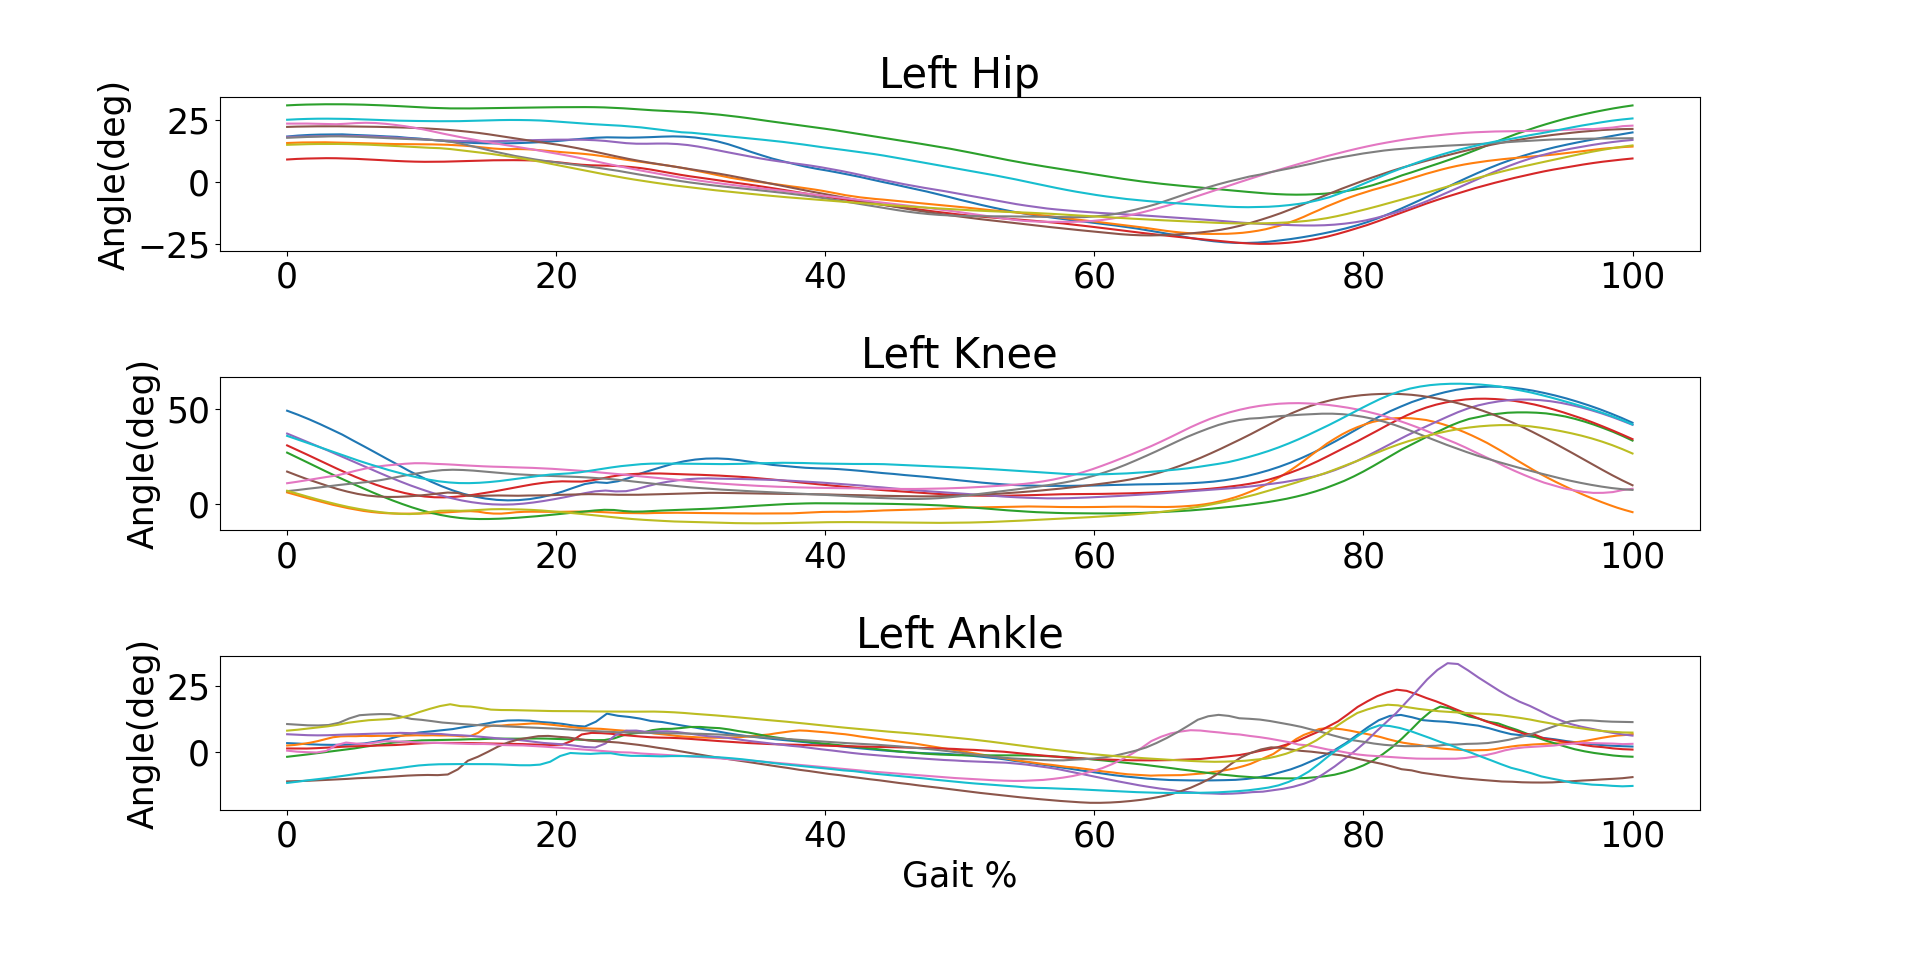
\includegraphics[scale=0.30]{images/gait_data/gaittraining.png}
    \caption[Raw Joint Trajectories Collected from the Subjects]{Neutral Joint With Markers}
    \label{fig:TrainingDemosGait}
\end{figure}

\begin{figure}[h]
    \centering
    \includegraphics[scale=0.060]{images/gait_data/Joint_direction_mocap.png}
    \caption[Gait Training Demos]{Joint angle markers and joint angle direction}
    \label{fig:TrainingJointPosition}
\end{figure}

TPGMM (\autoref{eq:MstepTPGMM}, \autoref{eq:EstepTPGMM}) was used to learn the motion of the trajectory. This unsupervised learning method allows for the features of the motion to be extracted for encoding. This method has not been used for learning and implementing gait motions as discussed in \autoref{sec:applfd}.  The advantages of this method are the following:

\begin{itemize}
    \item Allows the use of natural gait motions instead of hand-coded motion.
    \item Temporal scaling of the trajectory allowing for gaits to be slowed down or speed up.
    \item Spatial scaling of the motion allowing for the start and goal positions.
    \item Principled approach for the distribution of the Gaussians.
    \item Provides mixture model parameters for measuring the variance along with the demonstrations.
\end{itemize}


The BIC score was calculated for bin size 10-30 using  \autoref{eq:BIC}; due to the randomization initialization, the score and optimal bin size vary slightly. \autoref{fig:BIC} shows the BIC score for the bins sizes. On average, the optimal number of bins converged to learn the walking model is 15 bins.    

\begin{figure}
    \centering
    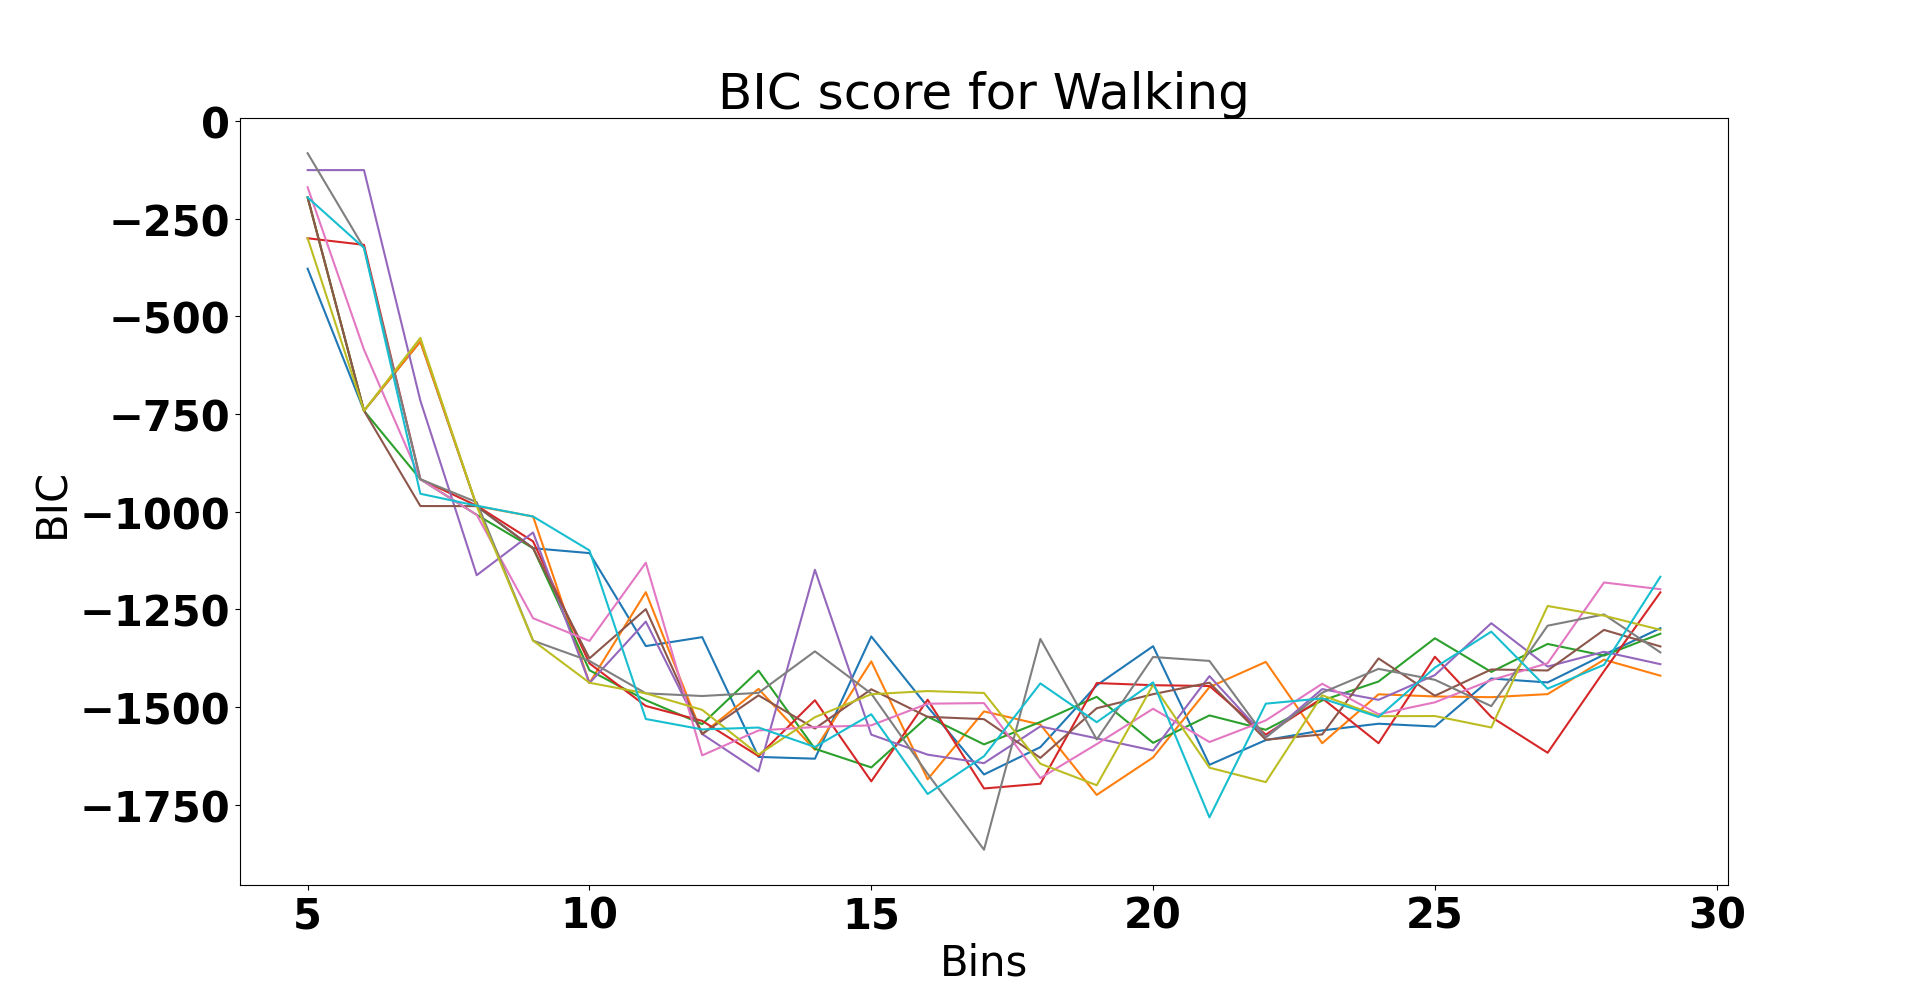
\includegraphics[scale=0.3]{images/gait_data/BIC_Walk.png}
    \caption[BIC Score for Walking]{The BIC Score that Determines the Number of Bins}
    \label{fig:BIC}
\end{figure}

The TPGMM process places the Gaussians that drive the system along the trajectory; this is shown in \autoref{fig:force}, the blue lines are the underline demonstrations transformed into a force.  The demonstrations were aligned using DTW. The red dots and green ovals are the means and covariances, and each oval is one of the bins (refer to \autoref{fig:cov_mat} for the calculations of the Gaussians).  GMR regresses over the means and covariances produced by the TPGMM process, accomplished through a superposition process of the overlapping Gaussians. The Gaussians with a smaller major and minor axis indicate a tight correlation, and the larger major and minor axis indicate less correlation of the points on the trajectory.  The Gaussians on the knee and ankle graphs have a slight variance along the demonstrations leading to small Gaussians. In contrast, the hip demonstrations have a more considerable variance leading to larger Gaussians. \autoref{fig:learnedModel} show the comparison of the learned model compared to the training demonstrations. The thin lines are the training demonstrations; the thick line is the trained model. The trajectories were extracted from the learned model above and used DMPs to reproduce each of the joints' trajectories. 


\begin{figure}[!h]
    \begin{subfigure}{\textwidth}
        \centering
        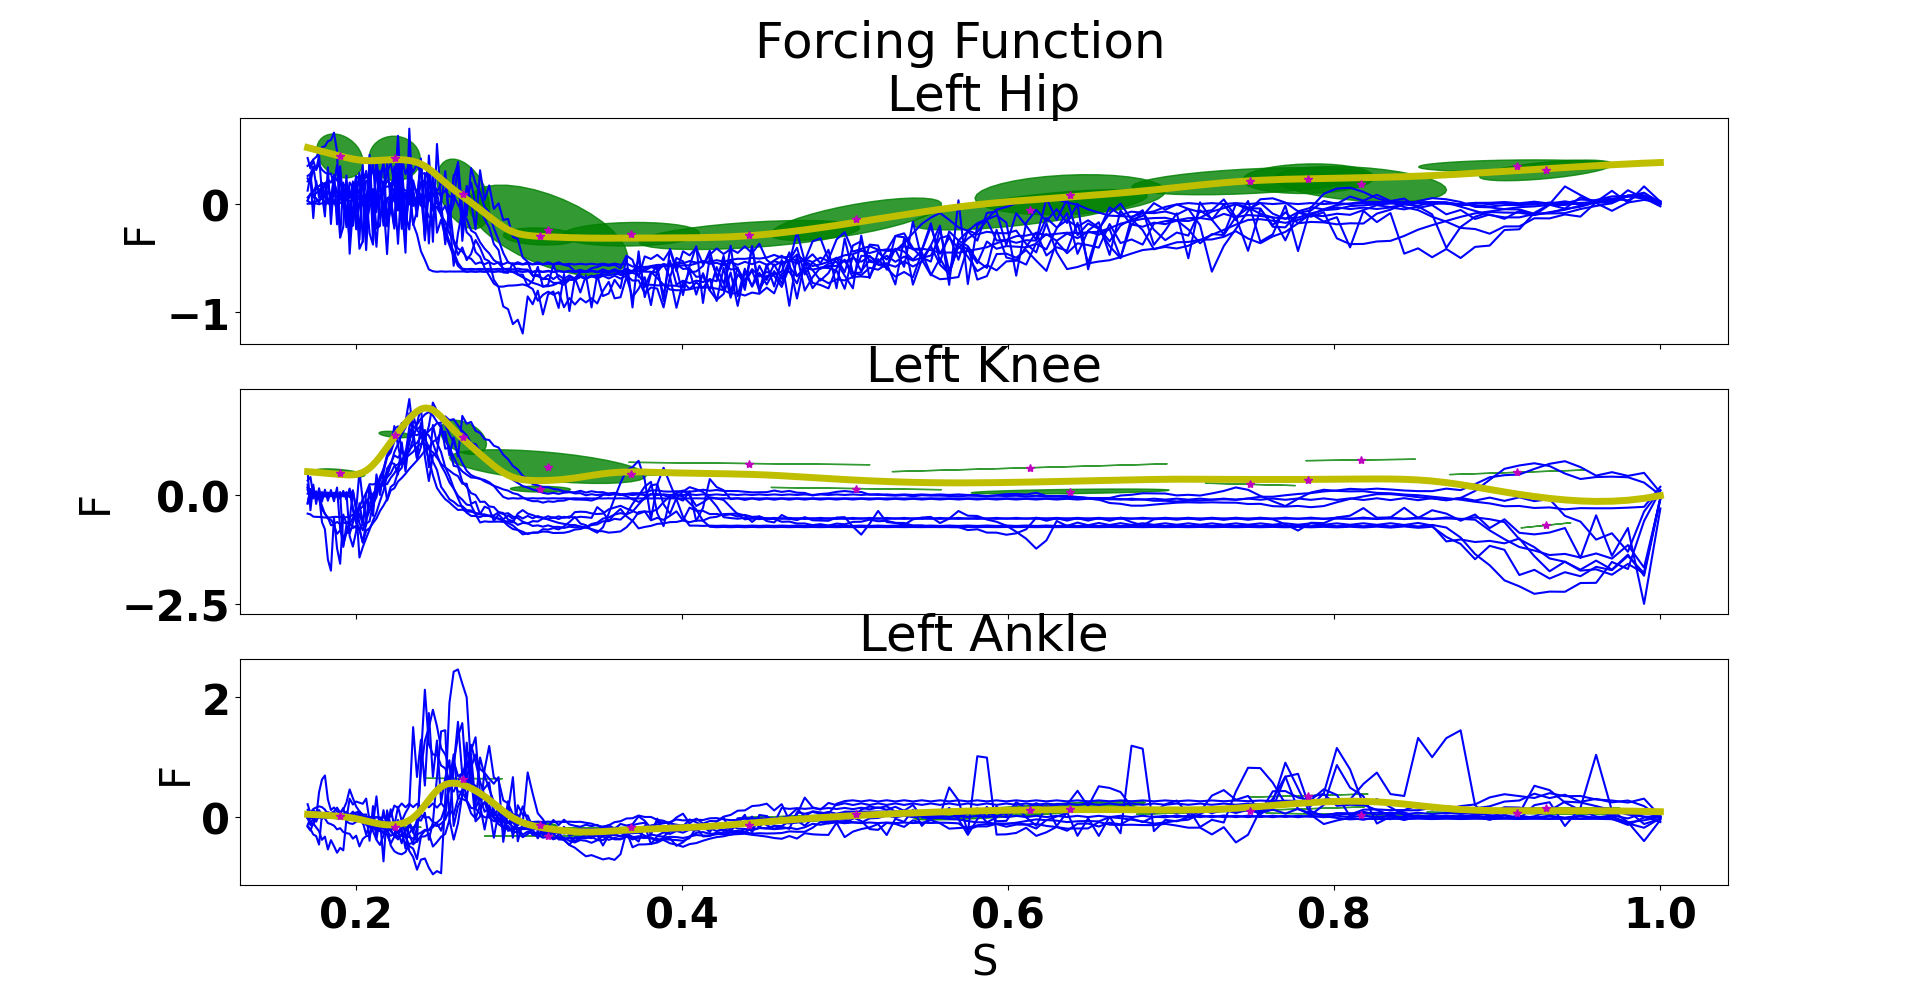
\includegraphics[scale=0.35]{images/gait_data/force_function2.png}
        \caption[Gait Forcing Function]{Forcing Function Learned for each of the trajectories. The red dots are the means and the green ovals are the covariances.}
        \label{fig:force}  
    \end{subfigure}

    \begin{subfigure}{\textwidth}
       \centering
    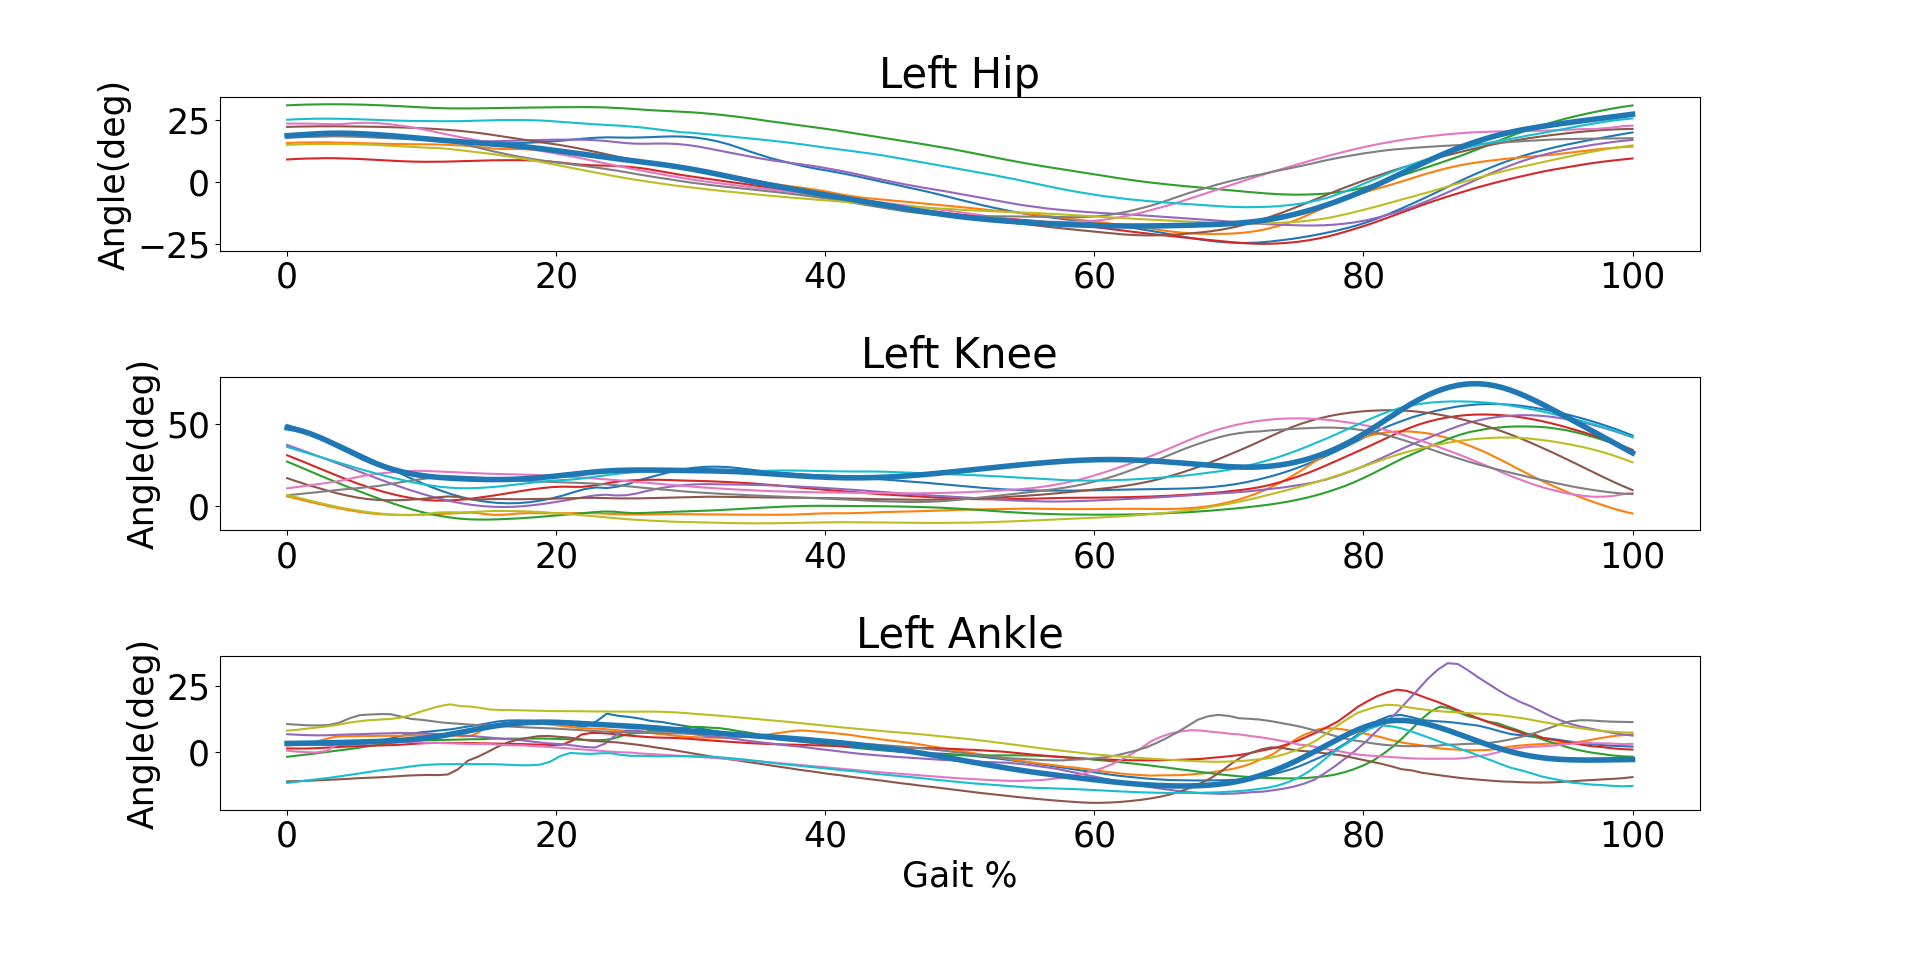
\includegraphics[scale=0.35]{images/gait_data/learnedModel.png}
    \caption[Learned Gait Model]{Learned model compared to the demonstrations. The thin lines are the demonstrations used to train the models. The thick line in the learned models.}
    \label{fig:learnedModel}
    \end{subfigure}
    \caption{Learning the gait trajectories}
    \label{fig:learninggaittrajectories}
\end{figure}





% \begin{figure}[h]
%     \centering
%     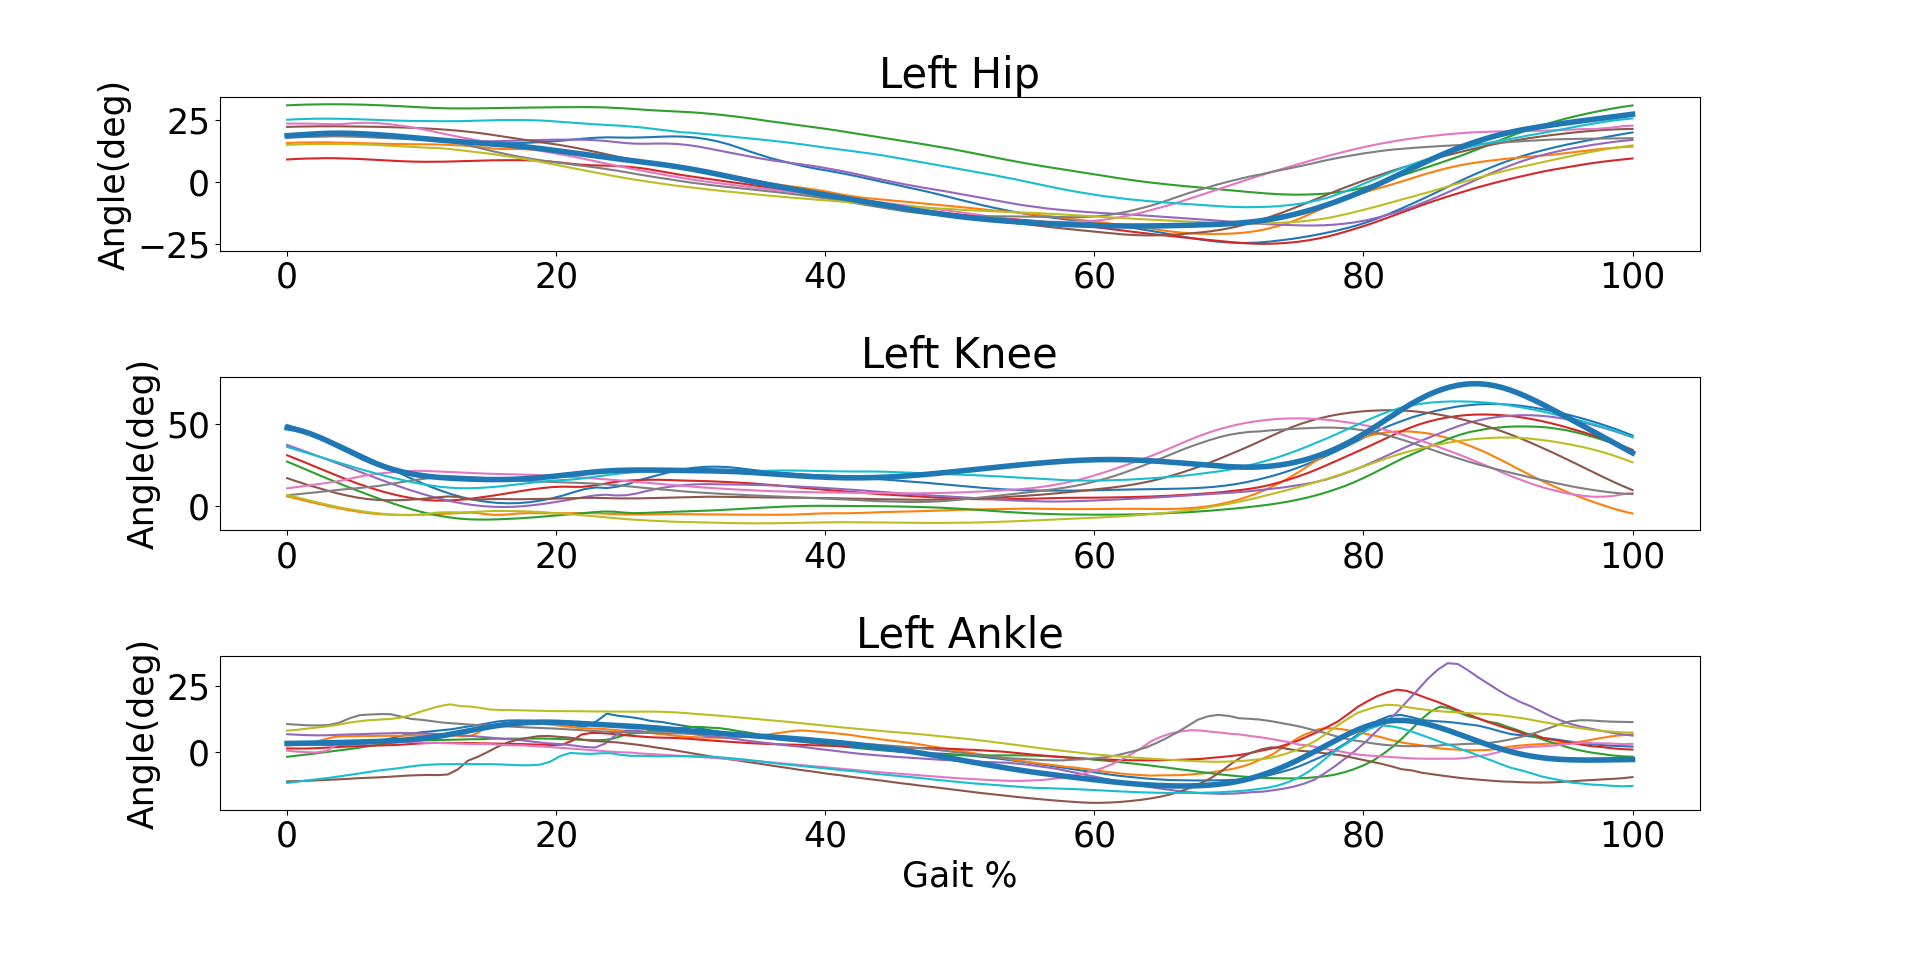
\includegraphics[scale=0.35]{images/gait_data/learnedModel.png}
%     \caption[Learned Gait Model]{Learned model compared to the demonstrations. The thin lines are the demonstrations used to train the models. The thick line in the learned models.}
%     \label{fig:learnedModel}
% \end{figure}

In addition to learning the joint angles, the forward kinematics of the leg were recorded by using the marker on the toe as a training source. \autoref{fig:learnedToe} shows the forcing function and replicated gait motion using a marker placed on the toe of the subjects—the $Z$ and $X$ axis as referenced in \autoref{fig:TrainingJointPosition}. The $Y$ was not learned since the system is contrasted to the sagittal plane. In all four graphs, the blue lines are the training demonstrations for the model. The green ovals in the upper two graphs are the Gaussians, with the red dot being the mean. In the lower two graphs, the black lines are replicated, motion model. Using BIC, it was determined that 7 was the optimal number of bins to use. AS shown in \autoref{fig:FK_BIC}, 3-15 bins were tested 10 times to ensure proper convergence and ensured that a local minimization was found. In all but two iterations, the BIC score remained identical. In the two remaining cases, the BIC score differed in the final bin size and did not affect the minimum BIC score.


\begin{figure}
    \centering
    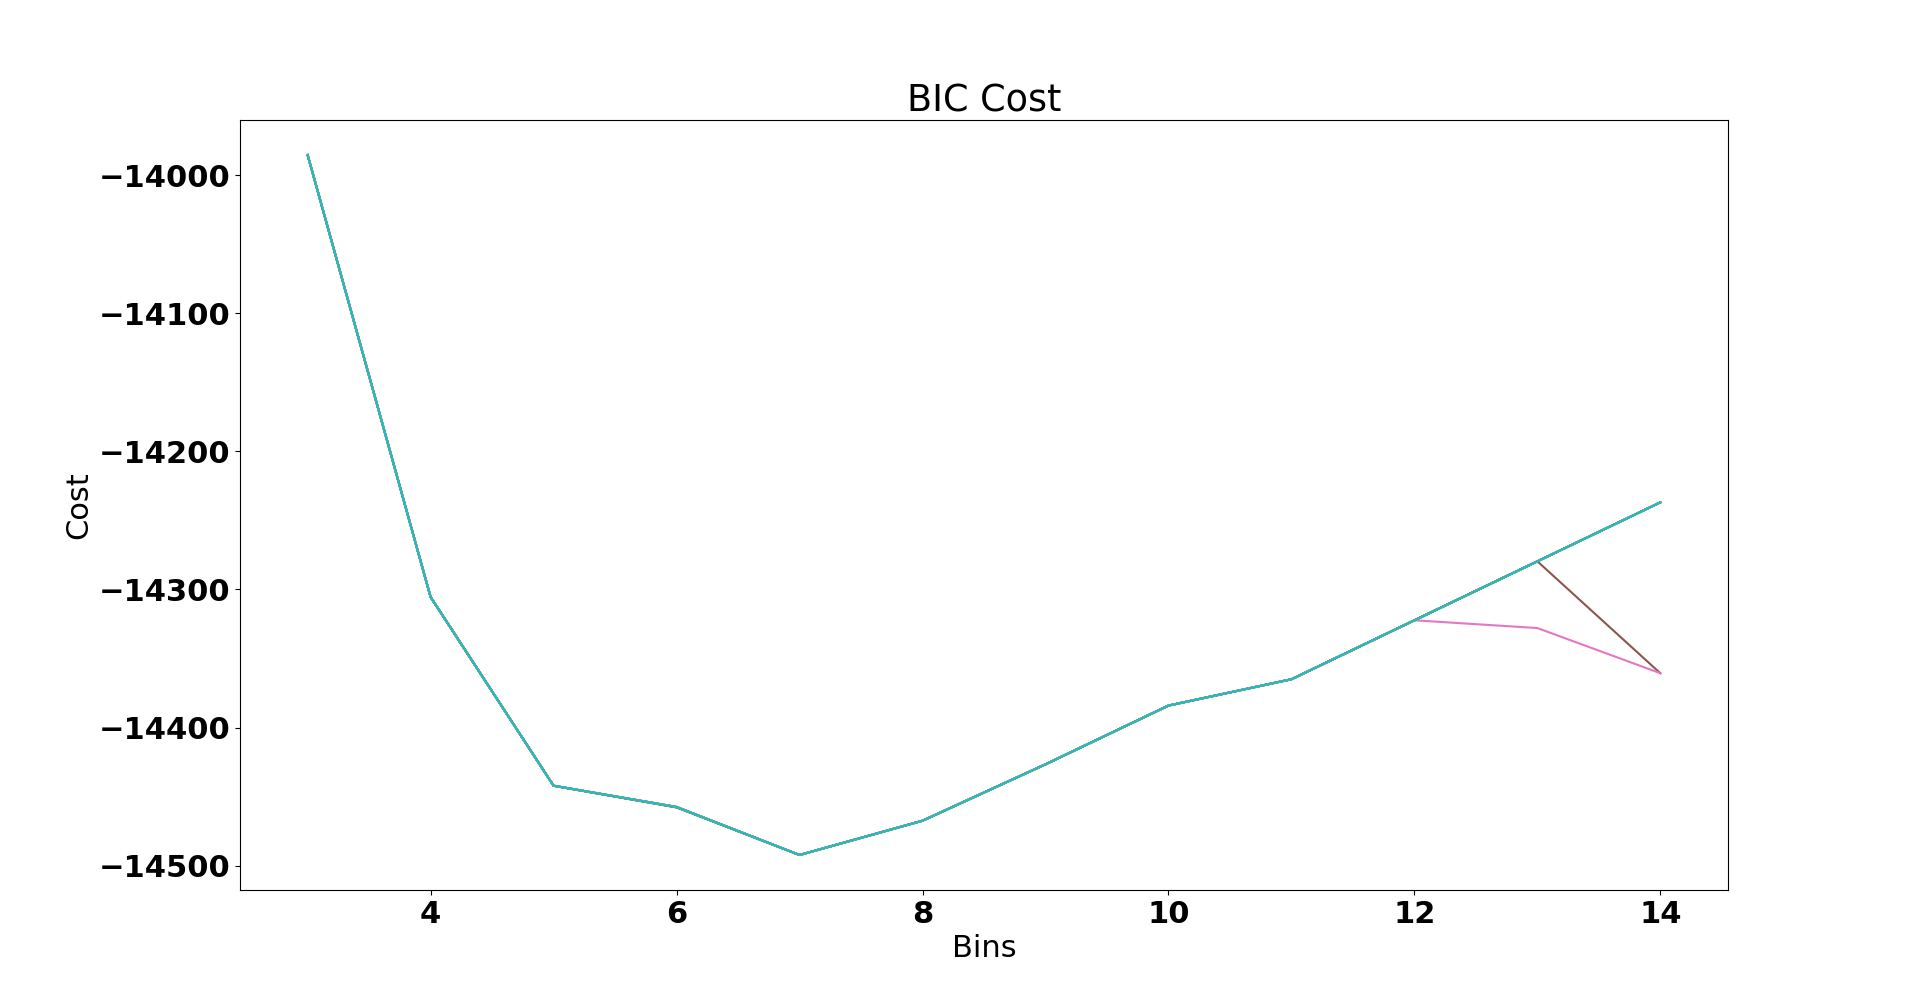
\includegraphics[scale=0.25]{images/gait_data/BIC_FK.png}
    \caption[FK BIC Score]{BIC score for Determining the Optimal Number of Bins for Learning the Fk Position of the Foot over a Gait Cycle}
    \label{fig:FK_BIC}
\end{figure}


\begin{figure}[!htb]
    \centering
    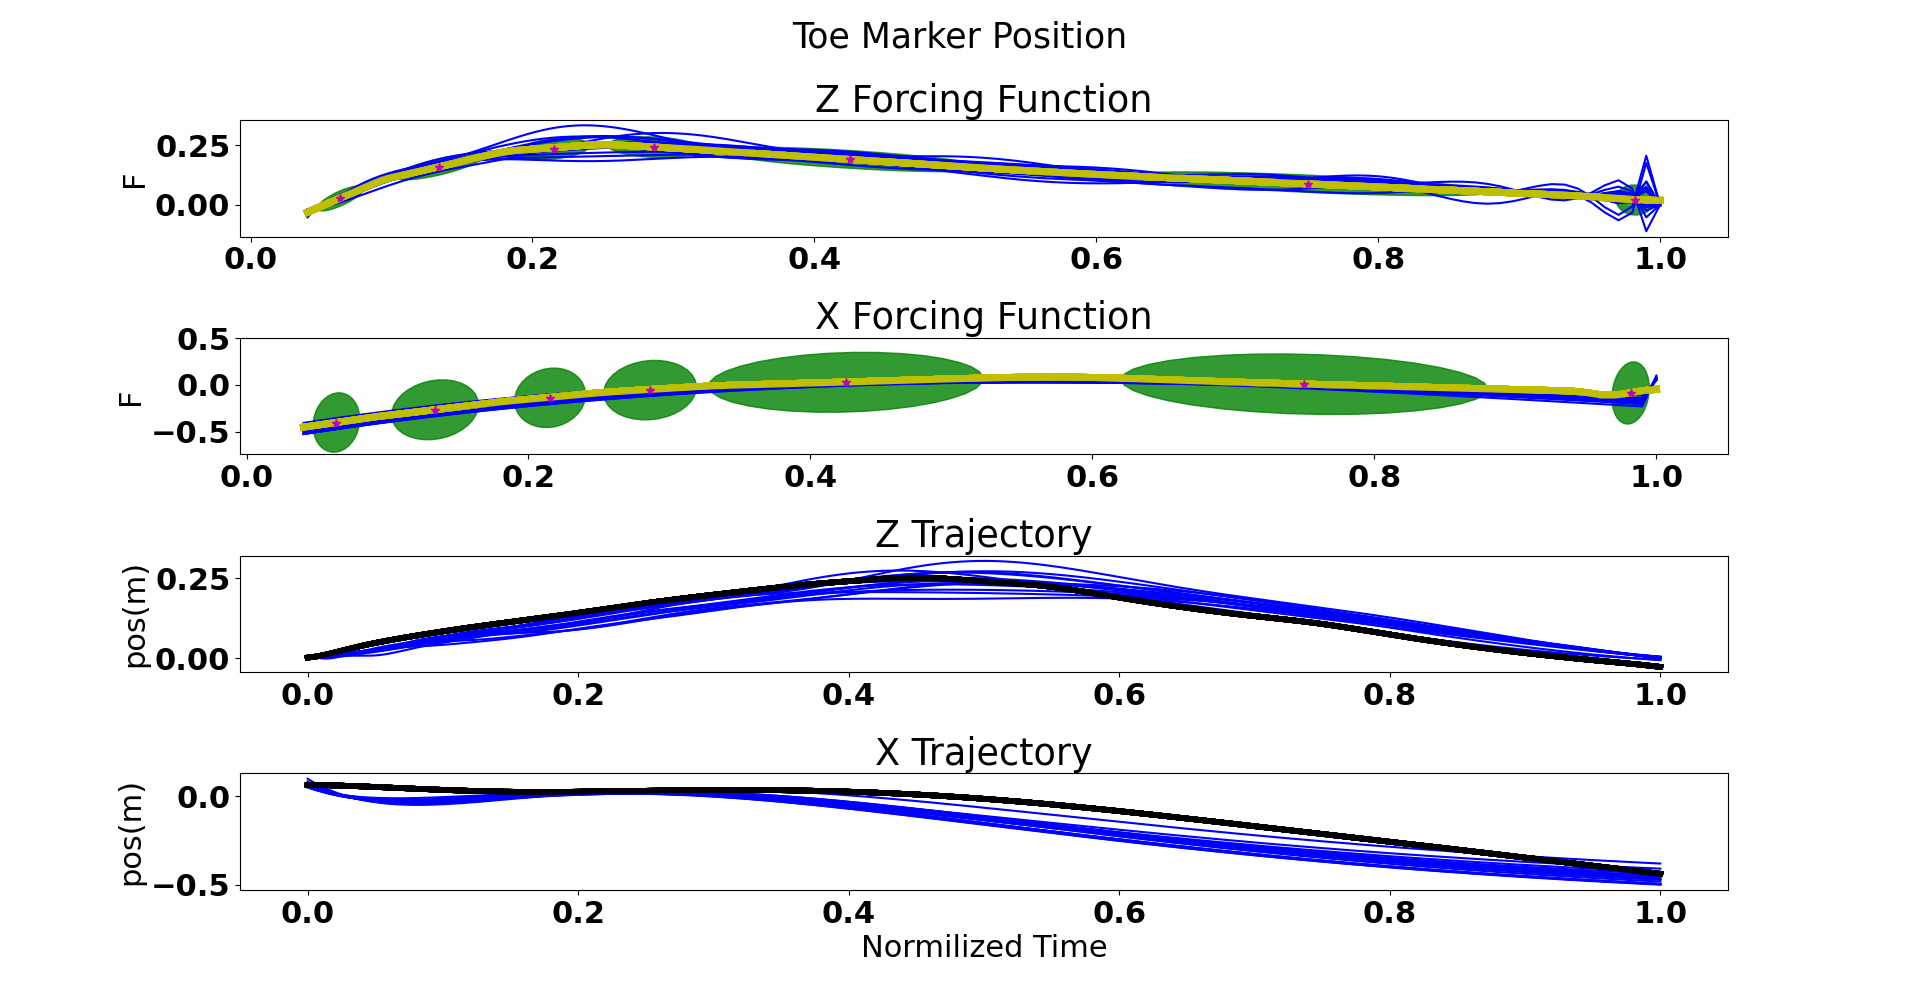
\includegraphics[scale=0.35]{images/gait_data/toe_maker_pos.png}
    \caption[Toe Marker Position]{Learning of the toe position during a single gait cycle, upper two graphs are the forcing functions. The lower two graphs are the replicated models an the training demonstrations.}
    \label{fig:learnedToe}
\end{figure}

Once the model is encoded using the tools discussed in \autoref{chap:software} can reproduce the joint trajectories. The processes to learn and reproduce the trajectories are separate systems allowing the encoding to be conducted offline and reproduced online. These models are used to generate the gait cycle for the exoskeleton in simulation. 


\section{Contributions}

All of the data collected was released open-source for community use and analysis. While there are other databases of gait motion out there, this data set provides additional information such as marker positions and joint torques. More markers and rigid bodies were used during the mocap trials than in past studies. The rigid bodies allow for analysis of leg the segment's relative motion. The raw marker position is valuable and can be used to observe the leg joints' forward kinematics. 

Additionally, an extensive database of stair climbing motions was released. This open-source database contains all the kinematics information of how people of different ages, gender, heights climb stairs. This database helps study how people adjust to climbing stairs and help program robots to reproduce this motion. The trajectories can be encoded and reproduced on a human-robotic system. 

The collected information was used to learn motion models that replicated gait trajectories in joint and task spaces. Both of which were optimized using BIC. Using the BIC score, the optimal number of bins was found to train the model. These generalized trajectories allow for various types of controls to be implemented. The generalized model will allow researchers to access lower leg models to be used on their own exoskeletons or legged robotic systems. 

\chapter{Vicon and Gait Analysis Software Package}
\label{chap:software}
\section{Overview}
The Vicon motion capture system collects a rich set of data for analysis and manipulation. This richness of this data set however makes the raw data difficult to extract and handle.
To handle this data is was pessary to develop a toolkit to parse the data into data structures that exposes the data to other APIs for manipulation and analysis. 

The Vicon  motion capture system is a popular motion capture system. This mocap system can export the data in several formats, including C3D \footnote{https://www.c3d.org/}  files and ASCII files. Vicon offers Python and Matlab packages to post-process the data; these packages only work on a computer with an active Vicon Nexus software package, making it challenging to work with the data. 

C3D files contain rich data that can be imported by popular biomechanical systems such as OpenSim \cite{seth2018opensim}. OpenSim will ingest the data and build an analysis model. The Biomechanical Toolkit offers a powerful tool for handling the raw C3D files to allow researchers to work with the mocap data and apply methods and algorithms \cite{barre2014biomechanical}. This package is written in C++, which is a compiled language, not an interpreted language. The advantage of an  interpreted language like Python is that it is easier to implement and code cane be executed on the fly. This is in contrast to C++ which has complex syntax with better computation performance \cite{varisteas2018distributed} \cite{bargiacchi2020ai}. Computational time is less of a concern when analysing data where a priority is more focused an obtaining results and extracting information then real time functionality.  The toolkit developed at Cleveland State University gait lab is an open-source tool for analyzing mocap data  \cite{DTK2014} \cite{GATK2014}. While, this package was developed in Python, this tool lacks flexibility and modulairty. The complexity of the toolkit makes it difficult to separate marker trajectories and handle marker analysis from gait data.   

To solve these problems a new toolkit was developed to manipulate and analysis Vicon and Gait data. Three software packages are presented, the Gait Core package, the Vicon Toolkit Package, and the Gait Analysis Toolkit Package. The software packages separate the tools for handling the Vicon marker data and the tools for gait analysis. This structure, shown in \autoref{fig:software}, allows for each software package to be used as stand-alone or in a unified system. The GaitCore package allows for a common API to be used along with constant data types.   

The three software packages are: 
 \textbf{GaitCore}\footnote{https://github.com/WPI-AIM/AIM\_GaitCore}, \textbf{Vicon toolkit}\footnote{https://github.com/WPI-AIM/AIM\_Vicon},  \textbf{Gait Analysis toolkit}\footnote{https://github.com/WPI-AIM/AIM\_GaitAnalysisToolkit} as described in \autoref{fig:software}. This was done to abstract the functionality and allow it to be used for different applications and mocap systems. The GaitCore package contains the low level APIs that build the data structures. The Vicon package contains APIs to parse and manipulate the raw mocap data. The Gait Analysis toolkit provides high level APIs to analysis gait trajectories and use them to build motion models. 

The advantage of these packages over similar packages is the underlining structure and modularity. This code base can be extend to handle other mocap systems which would then have access to the built in computation and analytical tools discussed below. The interpreted language also allows for researcher not familiar with C++ to quickly access and analysis their data. Then key functionality of the package is detailed below. The methods and algorithms used to build the package is also described. 




\begin{figure}
    \centering
    \includegraphics[scale=0.15]{images/software/software.png}
    \caption[Software Architecture]{Software architecture of the Vicon-specific toolkit for importing and processing data, the Gait Toolkit for motion anlaysis which is not specific only to Vicon, the GaitCore structure, and user applications.}
    \label{fig:software}
\end{figure}


\section{GaitCore}
At the center of the Vicon and Gait Analysis tool kit libraries is the GaitCore package. The GaitCore package provides low-level objects used in both the Vicon and Gait Analysis Toolkit packages. This package allows for the data to be manipulated and stored for consistent structures and readability.

The GaitCore package objects provide APIs to initialize the object and work with the data. Each class has override operators to allow for mathematical operations to be performed. The objects in the GaitCore package are the following:

\begin{itemize}[noitemsep]
\item \textbf{Core}:
\begin{itemize}[noitemsep]
    \item \underline{Point}: Holds a 3D point $(x,y,z)$, there are override operators and functions to perform basic vector operations. It can also be converted into a numpy array to perform more advanced operations.
    \item \underline{PointArray}: Holds a list of Point objects. This class provides functions to access to $X$, $Y$, and $Z$ axis. 
    \item \underline{Newton}: Holds angle, power, torque, force information that is calculated by the Nexus system. 
    \item \underline{Data}: Holds time sequenced data, it can be used to organize joint data against the time period. This class has two fields; data and time. It is a method of sequencing the data.  
\end{itemize}
\item \textbf{Bio}:
\begin{itemize}
    \item \underline{Joint}: Holds information on a single joint
    \item \underline{Leg}: Holds three joints (hip, knee, ankle)
    \item \underline{Arm}: Holds three joints (shoulder, elbow, wrist)
    \item \underline{Trunk}: Holds four joints (head, spine, thorax, plevis)
    \item \underline{Side}: Holds left and right side of the body
\end{itemize}
\end{itemize}




\section{Vicon Package}
\subsection{Overview}
The Vicon Toolkit Package parses and organizes the data exported by the Vicon Nexus software. The Nexus software exports an ASCII file with headers distributed throughout the row of the file. The Vicon parser extends an abstract base class \textit{Mocap}; this allows for abstract of the core functionality required for different mocap systems; this includes the marker interpolation and joint modeling. This allows the tools discussed to be used for other mocap systems like the Optitrack \footnote{https://optitrack.com/}.  
 The tools in this package are summarized below: 

\begin{itemize}[noitemsep]
    \item Gap filling of missing data 
    \item Organizing the data from the plug-in gait model 
    \item Sorting of rigid bodies
    \item Access to force plates and EMGs 
\end{itemize}


The Vicon Toolkit Package sorts the data into three buckets (classes): markers, devices, and model outputs. Each of these classes has internal functions for analysis. The classes were created to align the section headers in the ASCII file export from Vicon Nexus. 

The Vicon object is initialized with a single line of code. The only mandatory parameter is the path to the ASCII file; there are optional parameters for gap filling and interpolation of missing data. The interpolated data can be exported to a new file for later use.  \autoref{setup} shows how to initialize the Vicon object.

\lstinputlisting[language=Python, 
caption=This block shows how to initialize the Vicon object and use the interpolation parameters, label=setup]{code/set_up.py}


\subsection{Gap Filling}

A common complication during a mocap trial is that the cameras will lose track of one or several markers; this results in gaps in the data. The Vicon Nexus software provides several tools to pattern and spline fill missing marker data; this should fill most of the gaps. However, some gaps might remain in the exported data. These gaps need to be filled in before any analysis can be performed. Tools were build into the package to filling in and interpolate missing data. The tools are abstracted for the implementation and development of custom interpolation methods. The Vicon object will keep track of which values were interpolated. This was done so that user of this package can track what data was interpolated. 


There has been substantial effort put into the research and development of missing marker interpolation methods. Each method is designed under different constraints and is optimized for different scenarios, including but not limited to biomechanical research. These methods vary from simple spline fitting to complicated statistical methods. 

Akima spline interpolation \cite{wang2014real} is a simple polynomial interpolation method. The Akima method uses $3^{rd}$ order continuously differentiable polynomial. The Akima 's feature method's feature is it has a continuous $1^{st}$  order derivative through its endpoints and behaves well when the second derivative of the data is rapidly changing. \autoref{eq:akima} defines the the polynomial between the two points $(x_{1}, y_{1})$ and $(x_{2}, y_{2})$, with slopes $t_{1}$ and $t_{2}$ respectively. The Akma method is limited in several ways; it assumes that a polynomial can interpret the marker's movement. It does not consider the marker's velocity vector and does not consider the movement of other markers attached to the same body. 

\begin{equation} \label{eq:akima}
\large
\begin{split}
        y &= p_{0} + p_{1}(x - x_{1}) + p_{2}(x - x_{1})^{2} + p_{3}(x - x_{1})^{3} \\
        where, \\
          p_{0} &= y_{1} \\
    p_{1} &= t_{1} \\
    p_{2} &= (3(y_{2} - y_{1})/(x_{2} - x_{1}) - 2t_{1} - t_{2})/(x_{2} - x_{1}) \\
    p_{3} &= (t_{1} + t_{2} - 2(y_{2} - y_{1})/(x_{2} - x_{1}))/(x_{2} - x_{1})^{2}
\end{split}
\end{equation}

Piaze \textit{et. al} attempting to resolve some of the limitations pure interpolation buy considering the velocity vector of the marker and its recent history \cite{piazza2009towards}. This method assumes that a marker will either move locally in a straight line or a circle pattern. A backlog of markers is stored to find the forward vector of motion; this backlog is used to estimate a marker's velocity. Using both the linear and angular velocity, a local model of the marker can be found and used to interpolate to find small gaps in the marker's trajectory. This method is relatively simple in its implantation and execution. It takes advantage of the marker's prior motion to interpolate its future position and does not require the marker noise variance model. This method has several limitations; it only relies on a single marker, meaning that it cannot infer a marker's position from other markers. In addition, it assumes that all motion on a body can either be modeled as linear or circular, which may not always be the case. The velocity is also calculated by examining the backlog of the marker's location, while this leads to a vector be less subject to noise from frame to frame. It can lead to the velocity vector lagging behind the motion of the marker. 

McCain \textit{et. al} proposed a method that takes advantage of rigid bones in the human body and marker attached to the bones will have the same relative motion \cite{li2010bolero}. In this method a hard and soft assignment method was examined. The soft assignment method relaxes some of the assumptions of marker noise caused by skin movement. This method is based on the expectation-maximization (EM) algorithm and Kalman like filtering method; this is statistical-based method that requires knowledge of the marker noise and additional markers to work properly. 

A similar method was developed by Lasenby \textit{et. al}, this method also used a bone constraint method \cite{aristidou2013real}. However, this method did not constrain its movement to be linear; it replaced the linear Kalman filter with an unscented Kalman filter. An unscented Kalman filter allows for nonlinear models of the motion to be assumed. This method takes full advantage of the markers being attached to a rigid bone structure. It also uses a variable tune model with a target velocity and acceleration of the markers. The latter, however, is subject to too much noise to be computationally useful. This method requires three markers per body for tracking; these markers allow the marker to calculate the body's 3D location in space. While this number of markers would be common for biomechanical trials, it requires many markers to be used; this makes it unsuitable for trials with few markers or markers not attached to rigid bodies.

Each of the methods discussed above is optimal for different applications and research. Furthermore, new methods can be developed to produce better results or suit a particle application or research. To handle this the package was build so that the user can specify the desired interpolation method. This is unique among the other packages. Other packages either do not offer an interpolation method or it is fixed.  

\subsection{Rigid Bodies}

Rigid bodies in mocap are built from a collection of individual markers on a body segment. Three or more markers is required to define the position and orientation of body in space allow for the relative pose of the body to be found in all the frames. Using rigid plates with known marker position the marker placement can be set \footnote{https://www.vicon.com/hardware/accessories/}. This rigid bodies are strapped the person segments to record the positions of the body. \autoref{fig:markers_side} shows the coordinate frames on the leg of a person. \autoref{fig:rigidbody} shows the rigid body plate with marker locations. 

\begin{figure}
\centering 
\begin{subfigure}{0.4\linewidth} 
  \centering 
  \includegraphics[scale=0.05,frame]{images/software/marker_side_coor.png} 
  \caption[RigidBody Frames]{Rigid body frames on the leg} 
  \label{fig:markers_side} 
\end{subfigure} 
%
\begin{subfigure}{0.4\linewidth} 
  \centering 
    \centering
    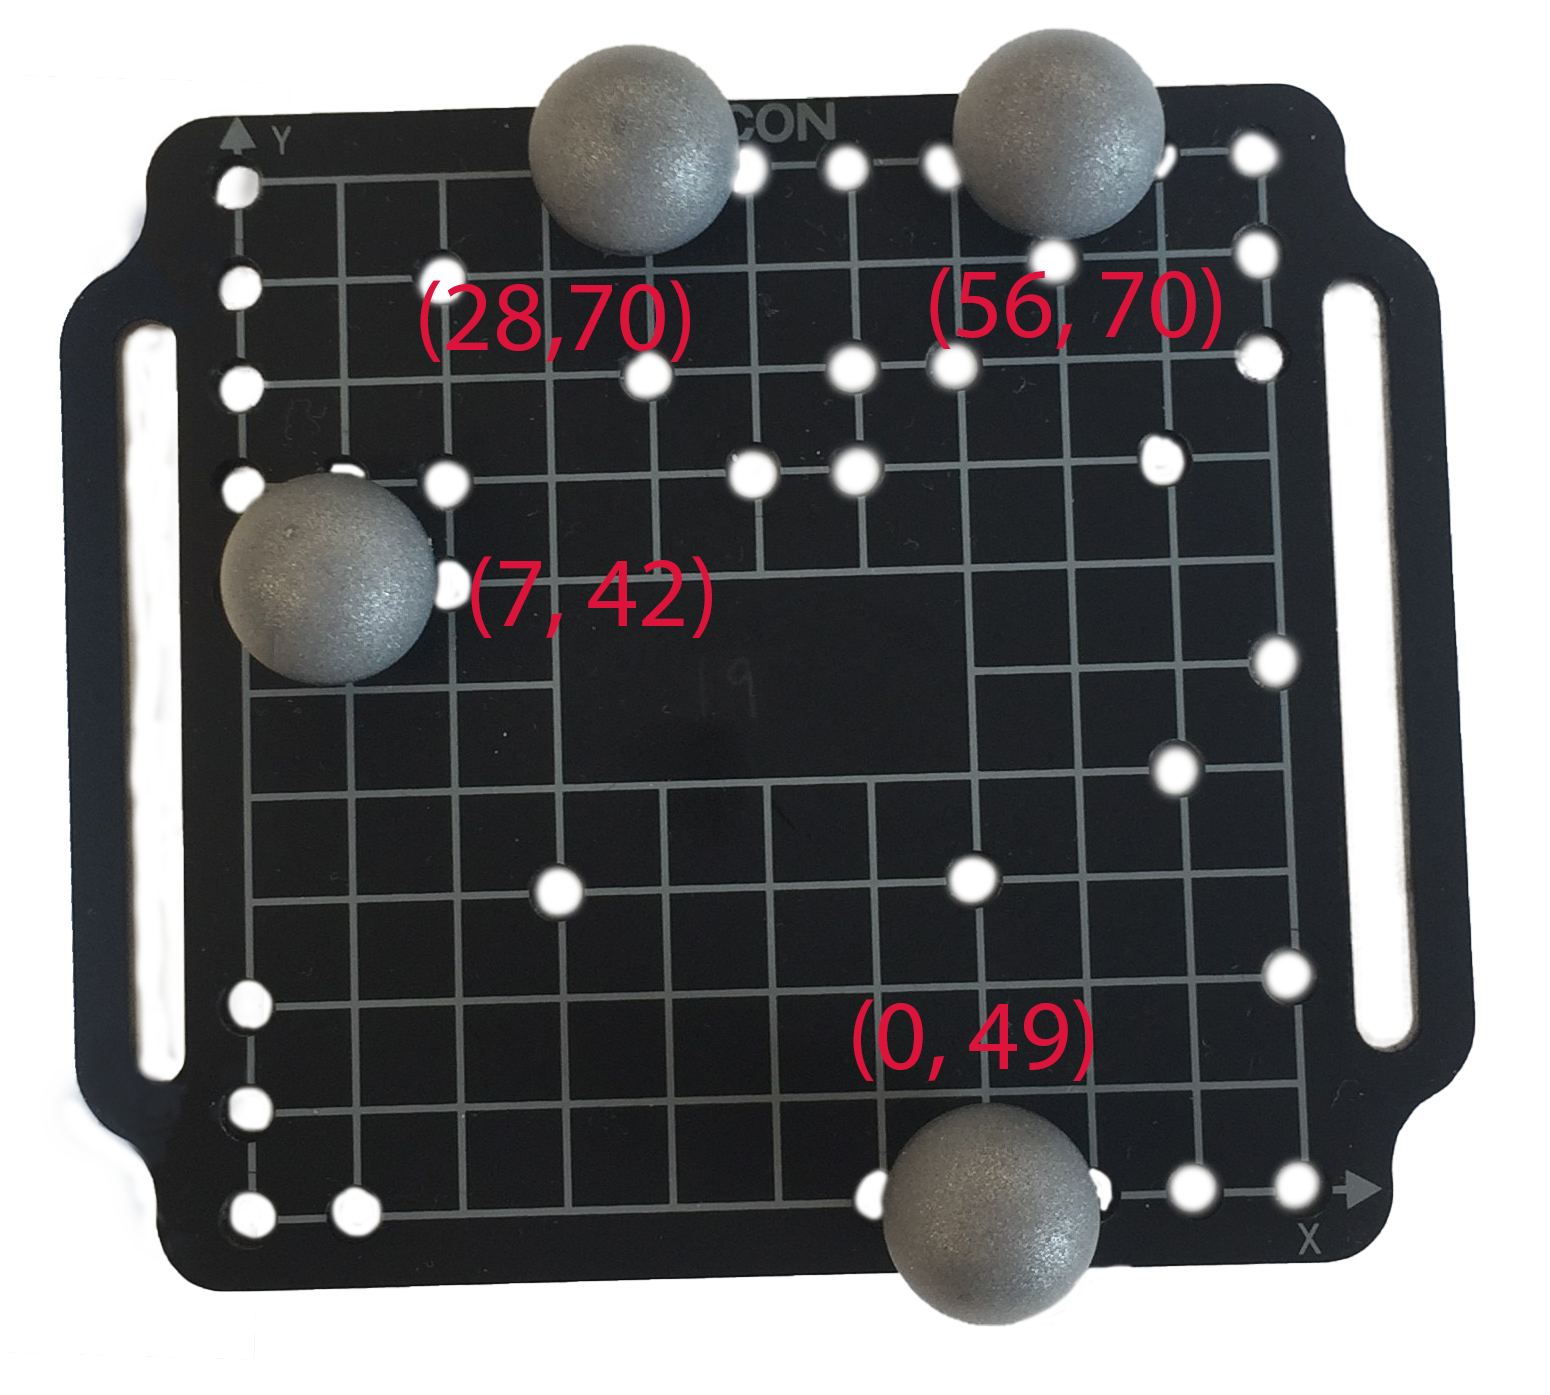
\includegraphics[scale=0.11]{images/software/rigidbody_label.png} 
    \caption{Labeled rigid body plate from Vicon}
    \label{fig:rigidbody}
\end{subfigure} 
\caption[Rigidbodies and Placement]{Rigidbodies and Placement} 
\label{fig:markers} 

\end{figure} 

A least squares method is used to the transformation be between the markers point cloud \cite{arun1987least}. Using this method the relative location of the markers is required, which is set using the rigid body plates. This is described in \autoref{eq:pointcloudtransformation}. In this equation $A$ and $B$ are the recorded locations of all the markers in different frames. The goal is to calculate the translation $t$ and rotation $R$ between the two point clouds. The rotation is found using Singular value decomposition (SVD). \autoref{eq:rotationPointclouds} is used to find the rotation. To isolate the translation component the marker point clouds are re centered around the origin by subtracting the centroid (\autoref{eq:centroid}) of the pointcloud. Here, $A_i$ and $B_i$ is a $3x1$ vector of the position ($[x,y,z]$) of a single marker. Using the rotation matrix $R$ the translation is then computed using  \autoref{eq:translationPointclouds}.  The error for every transformation is calculated and returned; it is used to evaluate the transformation's goodness of fit. \autoref{eq:errorPointclouds} is used to calculate the fit error.   


\begin{equation}
    \large
    RA + t = B
    \caption{Marker point cloud transformation}
    \label{eq:pointcloudtransformation}
\end{equation}

\begin{equation}
\large
    centroid_{A,B} &= \frac{1}{N} \sum_{i}^{N} \{A,B\}_i 
    \caption{Calculation of the pointcloud centroid}
    \label{eq:centroid}
\end{equation}


\begin{equation}
\large
    \begin{split}
        H &= ( A - centroid_A) ( B - centroid_B) ^T\\
    [U,S,V] &= SVD(H)\\
    R &= VU^T    
    \end{split}
    \caption{Finding the rotation matrix between the marker pointclouds}
    \label{eq:rotationPointclouds}
\end{equation}
    
\begin{equation}
    \large
    t = centroid_B - R \times centroid_A
    \caption{Marker point cloud transformation}
    \label{eq:translationPointclouds}
\end{equation}

\begin{equation}
    \large
    err = \sum_{i}^{N} || RA_i + t -B_i ||^2
    \caption{Error of the point cloud fitting}
    \label{eq:errorPointclouds}
\end{equation}


The Vicon toolkit will automatically gather markers into rigid bodies and can produce a transformation matrix for each rigid body for every point in the trial. The transformation are used to locate relative movement between the various bodies. The novelty of this package is its flexibility to generate rigid bodies from a set of markers. The package handles the gather of the markers on the same body and due to the abstraction layer, it can be used for any mocap system. 


\subsection{Addition Features}

\subsubsection{Model Outputs}
The Vicon Nexus software has several plug-in models (upper and lower) for fitting marker data to the human's body. The plug-in models are used for calculating the joint angle, torque, power, and force output by the plugin model. These values are critical for analysis of gaits and human motion.  The Vicon package stores all of this data in the Newton class. The joint class stores the data for a single joint, such as the hip, shoulder, or knee. This structure allows for easy access to the joint kinematics and dynamics. \autoref{modeloutput} shows how to get the left hip angle of a subject while walking. By replacing angle with the moment, the torques around that joint can be accessed.


\lstinputlisting[language=Python, 
caption=This block shows how to get the hip angle around the $X$ axis of the course of the entire trial, label=modeloutput]{code/modeloutput.py}

This package makes provides single line access to all the model output information. Using the model output information the joint trajectories of the gait cycle can be studied and used for developing motion models. All the critical information is provided to the user.  



\subsubsection{Visualization of Trial}
The \textit{play()} function generates a 3D plot of every marker position through time. \autoref{fig:playFigure} show a frame from the \textit{play()} from a trial where a subject climbed a staircase. Markers and rigid bodies were placed on the subject's legs, and a rigid body was placed on each of the steps of the stairs to locate each of the steps. The Vicon object also has a graphing method that will create and plot a selected field graph.

\begin{figure}
    \centering
    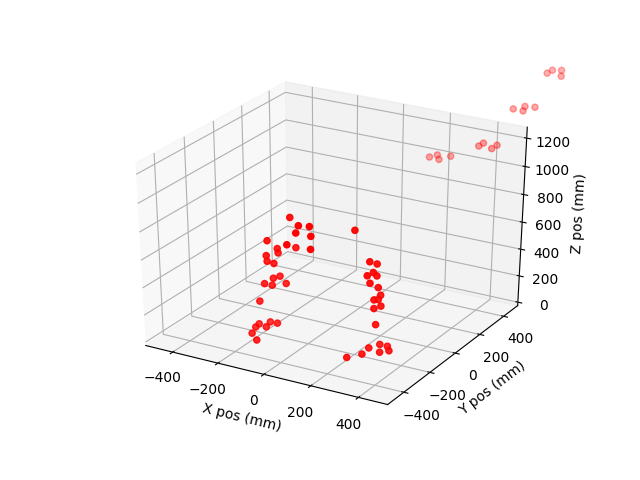
\includegraphics[scale=0.6]{images/software/play.png}
   \caption[Play Figure]{Marker locations in a single frame during a trial of climbing stairs. Each of the red dots is a marker. The marker clusters on the right hand side are rigid bodies placed on each stair. }
    \label{fig:playFigure}
\end{figure}


\section{Gait Analysis Package}

\subsection{Overview}
While the Vicon package provides broad tools to handle the mocap data; the Gait Analysis Toolkit provides more focused tools to handle gait analysis. This package includes: 
\begin{itemize}[noitemsep]
    \item Separating gait cycles
    \item Comparing different subjects gaits
    \item EMG filtering
    \item Learning of gait trajectories
\end{itemize}

These tools were developed to compare the gait motion collected during the trial. The toolkit will separate the gait motions into individual gait cycles. The gait cycles can be compared within the trial or against other trials or subjects. This allows for features of the trajectory to be compared to find patterns. 

\subsection{Gait Detection}
\autoref{fig:gaitDetection} show the extract gait cycles. It analyzes the first and second derivative to find the max peaks and inflection points. This joint angle method can lead to a slight phase shift in a gait cycle; this can be improved using information from the force plates. Once the index of all the gait cycles is found, the devices data and the model data associated with the gait trail are separated by the indices. Each of the lines is a gait cycle extracted from a separate subject. 

\begin{figure}[h]
   \centering
    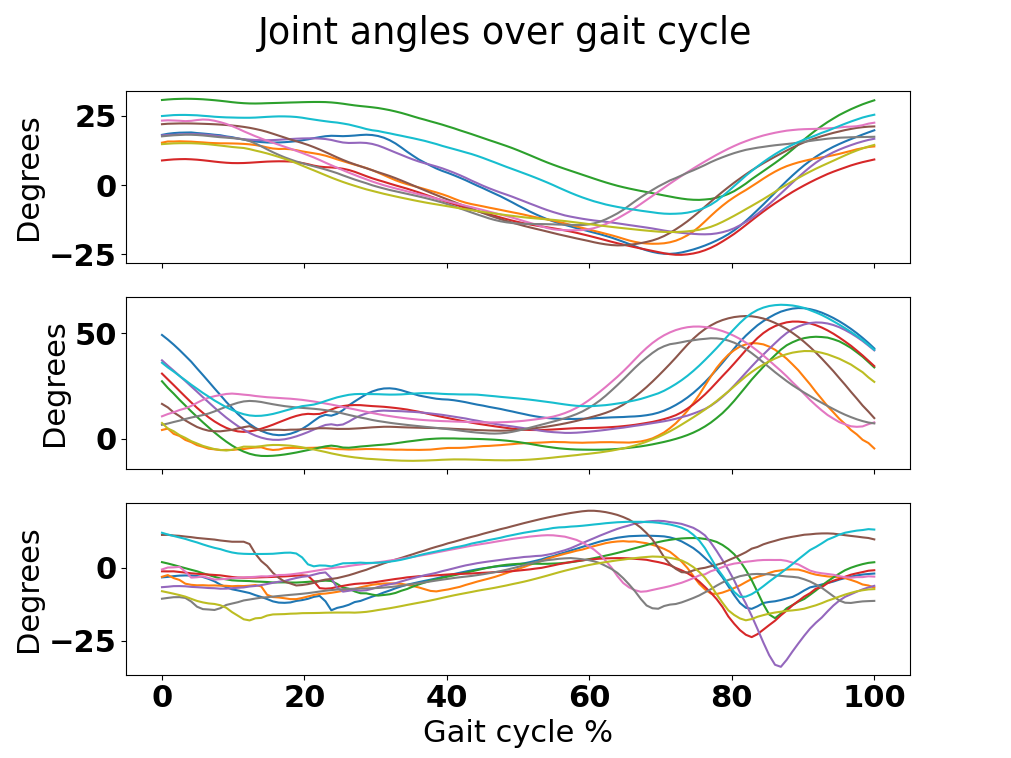
\includegraphics[scale=0.5]{images/software/gaitcycle.png}
    \caption[Gait Cycles]{The joint angle during a gait cycle. Each line represents a different subjects gait. The trajectories were re-sampled to be the same length}
    \label{fig:gaitDetection}
\end{figure}



\subsection{Learning from Demonstration}

The LfD algorithms are built into this package to learn the record bio-mechanical information. This allows for seemly flow from data collection to replication. \autoref{fig:flowchart} shows a flowchart of how a trajectory can be learned. \autoref{fig:learned} shows a learned demonstrations and the learned trajectory. The software are based on the other open-source packages \cite{calinon2016tutorial}. These other package while perform the mathematical operations, they are difficult to use without outside their provided data set with the code base. 


\begin{figure}
    \begin{subfigure}{0.4\linewidth} 
        \centering
        \captionsetup{justification=centering}
        \centerline{
        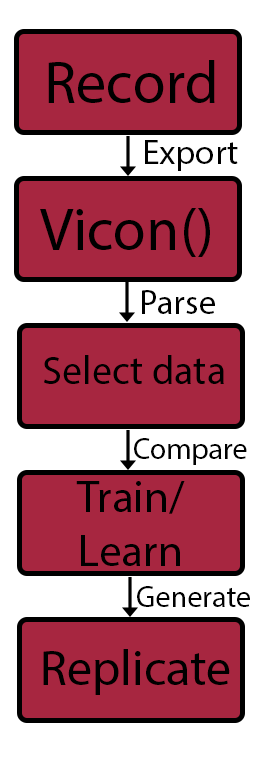
\includegraphics[scale=0.25]{images/software/flowchart.png}}
        \caption{Learning flow chart}
        \label{fig:flowchart}
    \end{subfigure}
    %
    \begin{subfigure}{0.4\linewidth} 
        \centering
        \captionsetup{justification=centering}
        \centerline{
        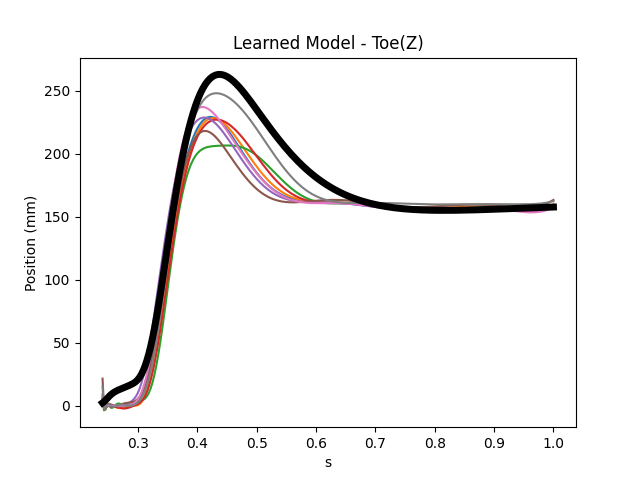
\includegraphics[scale=0.50]{images/software/learnedZ.png}}
        \caption{The thick line is the learned trajectories. The thin lines are the demonstrations that were used to train the model. This model was trained to replicate the toe marker}
        \label{fig:learned}
    \end{subfigure}
    
    \label{fig:my_label}
\end{figure}




The Gait Analysis package takes a different approach by provided the tools to parse data and build the data structures the user only has to provide the data set and have a basic understanding of Python. Another advantage of approach is the separation of the learning and replication systems. As discussed in \autoref{sec:lfd} the learning phase is an offline process. Using GMM to encode a data set can take several seconds to several minutes depending on number of demonstrations, length of the demonstrations, and the number of bins used to encode. This makes is desirable to use a powerful computer to encode the demonstrations. The replication of the trajectory with GMR is an online process using the parameters calculated by GMM. 

This separation of layers allows for the demonstrations to be learned once then can be played back later. The object-oriented approach reduces the amount of redundant code required. The package divides the tools into three parts allowing for additional algorithms to be developed and use the underlying structure: 

\begin{itemize}[noitemsep]
    \item \textbf{Model:} The main body of the algorithm, all the functions for handling the data. Examples of Models include (Gaussian Mixed Models(GMM), Gaussian Mixed Regression (GMR), Dynamics Motion Primitives (DMP), Task-Parameterized Gaussian Mixed Models (TPGMM). All of the Models extend the ModelBase class. This parent class contains properties and common functions to make it easy for future development
    \item \textbf{Trainer:} This class handles the process of organizing and processing the data. The trainer's classes all extend the base TrainerBase class, which has core functionality to parse and save the data. The trainer class will handle all the alignment and put the data in the model's proper form. The trainer pickles \footnote{https://docs.python.org/3/library/pickle.html} the model to be used later without needing to retrain the model. 
    \item \textbf{Runner:} The runner class plays the imitation model. The input to the model is the pickle file generated by the trainer. All the runners extend the RunnerBase class. This running method allows for feedback into the system. 
\end{itemize}


\section{Contributions}

The software packages presented have been release open source for community use and development. The packages can be installed using pip for easy of use. The modularity of the packages allows for the underlying tools to be used to build parsers for other mocap systems like the OptiTrack \footnote{https://optitrack.com/} mocap system. The Vicon Toolkit Package parses and provides convenient tools for access and manipulation of the mocap data. This package includes access to the raw marker position and allows for the manipulation of rigid body transformations. The Gait Analysis Toolkit provides tools for gait analysis independent Vicon package.  It contains a tool for extracting cycles, gait comparison, EMGs analysis, and learning and comparing trajectories. The contributions of the packages are the following:

\begin{itemize}
    \item Open Source tools for handling mocap data.
    \item Improved methods to handle and analysis marker and rigid body data by allowing rigid bodies to be defined and automatically finding transformation between different bodies in every frame.
    \iten Visualization tools to observe the marker position and calculated joint centers. 
    \item Comprehensive tools for learning from demonstrations to encode and reproduce biological motion. The encoding method is separated from the reproduction method allowing for offline learning and online reproduction.
    \item Modular method to fill in missing marker gaps allowing different gap filling methods to be implemented. 
    \item Built in tools to parse and compare gait trajectories. \item APIs to provide access to the lower and upper body plug-in Vicon models. 
\end{itemize}

All of the toolkits presented here were built to handle all the collected human demonstration data in \autoref{chap:gaitdata}. This allowed for the gait cycles to be extracted and compared. The collected data was then easily encoded using the built in LfD tools. The separation of the layers allows the trajectories to learned offline and replicated online. This feature was be used to build the simulation of the exoskeleton in \autoref{sec:sim}.



\chapter{Mechanical Design}


\section{Introduction}
The design of LARRE was inspired by the modular design presented by Bartenbach \textit{et. al.} \cite{7523699}.  Aliman \textit{et. al} also comprised a survey of all the existing lower limb exoskeletons currently in development; the survey gave further insight into the choice of actuators and sensors \cite{aliman2017design}. The Bartenbach design outlined the basic structure for the rehabilitation exoskeleton and improved by integrating additional sensors from the Aliman survey into the system. Additionally, the ankle-foot orthosis was moved to an overshoe joint to allow the system to don and doff with greater ease.
LARRE was designed to be a modular testing platform. Here we define modular as the ability to adjust to a person and allow for the swapping out of the joint mechanisms. LARRE's design fits the following requirements. 


\begin{enumerate}[noitemsep]
\item \textbf{Data Driven}: The kinematics and dynamics of the joints are defined by the biomechanical data. The joints must have the power to compensate for the mass of the person and the exoskeleton. 
\item \textbf{Adjustable}: The exoskeleton must be adjustable to fit the different people in order for the exoskeleton's joints to align properly to avoid putting unnatural force on a person's joints. 
\item \textbf{Modular}: The exoskeleton requires removable joints to allow for different joints testing and experimentation; therefore, universal connectors are needed to allow the swapping out of the joints. 
\item \textbf{Easy to build}: The exoskeleton needs to be easy to manufacture and assemble. The exoskeleton should be constructed from off-the-shelf material to allow researchers to build their testing and development systems. 
\item \textbf{Easy of Use}: The exoskeleton needs to be easy to use for both the clinician and the person wearing the exoskeleton. 
\end{enumerate}

 \autoref{fig:Render} shows an annotated rendering of LARRE.  Each of the major components is discussed in detail in  \autoref{sec:hip}, \autoref{sec:knee}, and \autoref{sec:ankle}. While LARRE was designed to work as a single system, the modality allowed each joint treated as a separate component and be independently designed and tested. 

\begin{figure}[h!]
    \centering
    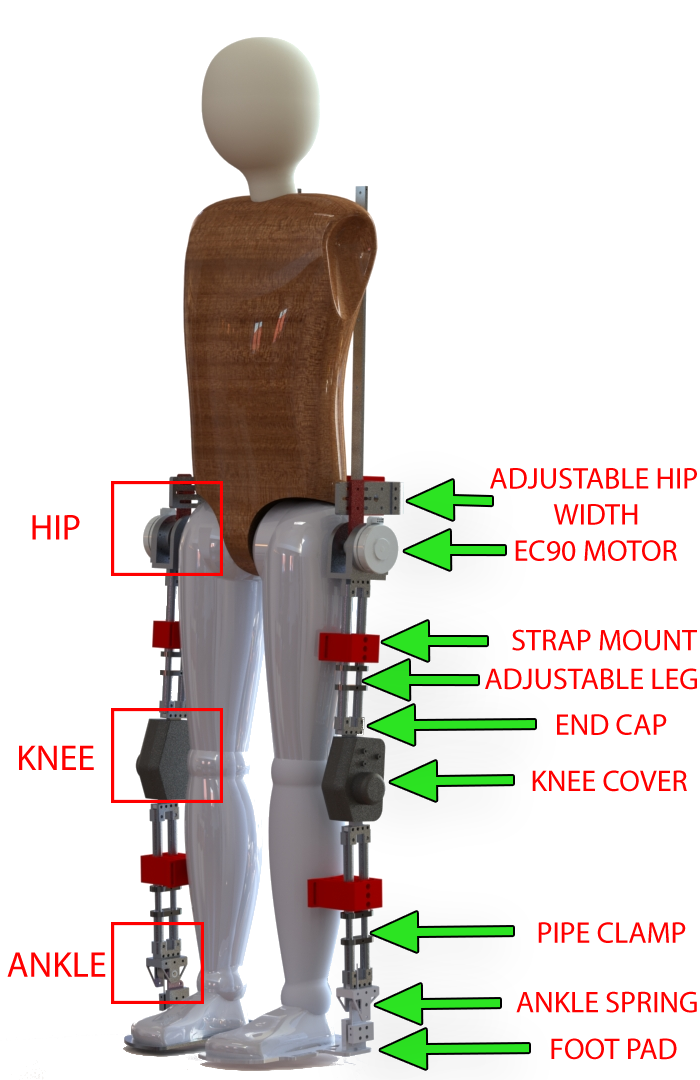
\includegraphics[scale=0.25]{images/mech_design/rendering2.png}
    \caption{Rendering of exoskeleton.}
    \label{fig:Render}
\end{figure}


\section{Hip Orthosis}
\label{sec:hip}

\autoref{fig:hip} shows an exploded rendering of the LARRE hip. The hip has an extension plate to expand the hips' width; they slide apart and lock with bolts. The bars along the person's back hold the battery box and support the person's upper body. A tactical vest \footnote{https://www.harmonicdrive.net/products/rotary-actuators#5071} and belt \footnote{https://tacticalgear.com/condor-gen-ii-battle-belt-od-green?hp=y}  straps the person into the exoskeleton. This vest and belt were chosen due to their high strength and padding, allowing them to support the exoskeleton's weight and avoid bruising the person. The belt is connected to LARRE and provides trunk support to help align the hip joints. The hips joints slide back and forth to align LARREs joints with the joints of the person.


\begin{figure}[h!]
    \centering
    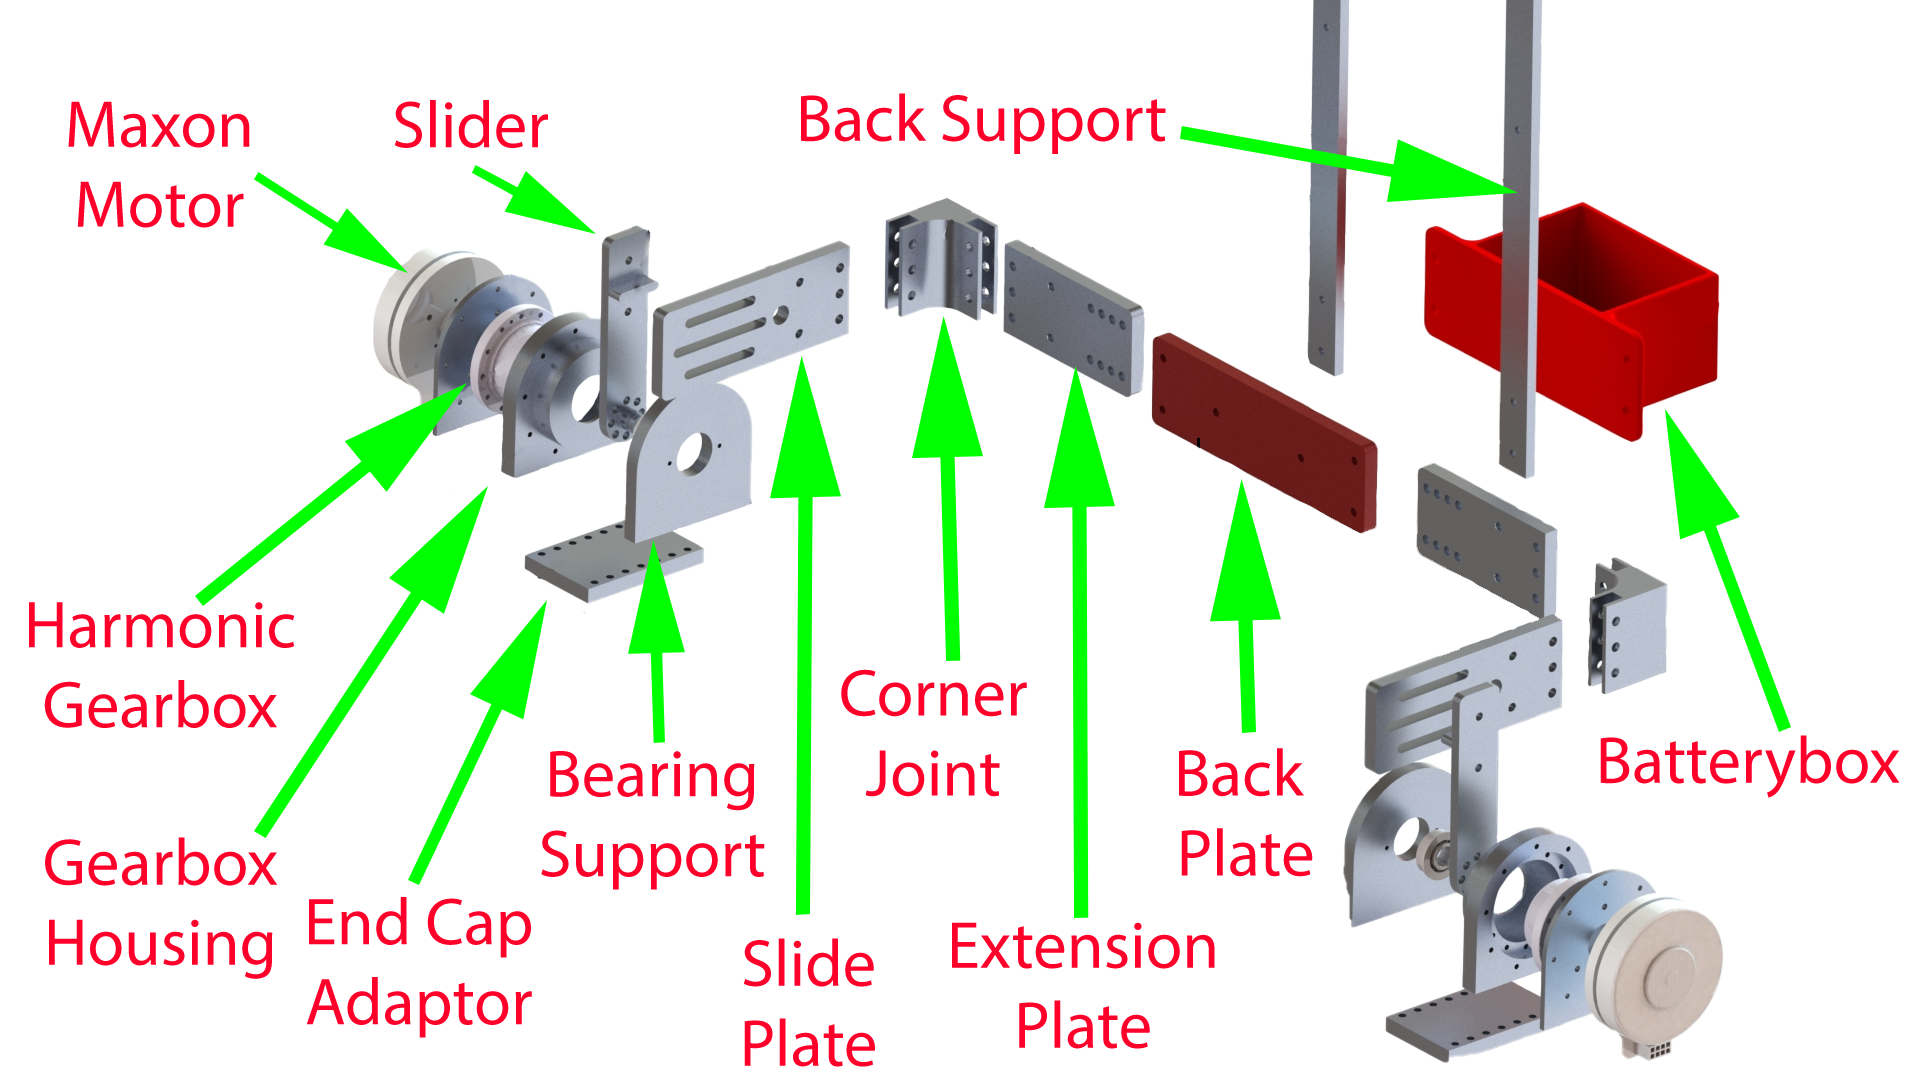
\includegraphics[scale=0.15]{images/mech_design/hip.png}
    \caption{Exploded Hip Mechanism}
    \label{fig:hip}
\end{figure}

LARRE is designed to be either passive or active. The passive mode allows the LARRE to be worn and collect data without controlling the motors. The passive version of the exoskeleton has been built for proof of concept. 

The active mode of the LARRE uses Maxon EC90 flat motors \footnote{https://www.maxongroup.com/maxon/view/product/motor/ecmotor/ecflat/ecflat90/505592} connected to Harmonic gearboxes \footnote{https://www.harmonicdrive.net/products/rotary-actuators#5071}. The Maxon motors are compact and have a low profile and built-in encoders. This motor is ideal for use in exoskeletons since it is a hollowed shaft gearbox that does not increase the exoskeletons' width. The encoders allow for positional control of the motors. Harmonic gearboxes reduce backlash and provide a 100:1 gear ratio. The active mode has been designed but left for future work to implement. 

This platform's modality makes it ideal for testing different orthosis on account of its' ability to easily switch the joints to test either a passive or active exoskeleton. The hip also acts as the base for the other joint that will be discussed below. 



\section{Wrap Spring Knee Orthosis}
\label{sec:knee}


Knee orthosis, despite the body of literature, only a few report the essential quantitative measurements, such as static or dynamic torque, safety, weight, and size. The lack of critical information made it difficult to arrive at design criteria. The design of the knee orthosis was based on the design criteria and the trade study found here \cite{subra2020design}. In the trade study, each criterion was assigned a different weight of importance, totaling 100 points, and allowed for the mechanism and parameters for the knee orthosis to be selected. The study concluded that a wrap spring clutch mechanism was the best design due to its highest score. The results are summarized in \autoref{tab:trade}.


\begin{table}[h!]
  \begin{center}
    \begin{tabular}{c|c|c|c} % <-- Alignments: 1st column left, 2nd middle and 3rd right, with vertical lines in between
      \textbf{wrap spring} & \textbf{motor} & \textbf{gears/clutch} & \textbf{cables} \\
      \hline \hline
      832.5 & 627.5 & 752.5 & 675.0 \\
      \hline
      \textbf{SEA}  & \textbf{Wafer disks}  & \textbf{Mag Damper} & \textbf{Hydraulics} \\
      \hline \hline
      592.5 & 805.0 & 757.5 & 580.0\\
    \end{tabular}
  \end{center}
      \caption[Knee Trade Study]{Summery of trade study}
    \label{tab:trade}
\end{table}


A wrap spring clutch mechanism is a quasi passive mechanism that allows for high holding torques \cite{irby1999optimization} \cite{tung2013design}. It consists of an arbor that is concentric with a wrap spring. \autoref{fig:WrapSpringClutch} illustrates how a wrap spring clutch mechanism works. The arbor is designed to have a slightly larger diameter than the spring. The friction between the arbor and spring prevents the arbor from rotating. When the leg's spring is actuated, the spring's diameter increases, allowing the spring to rotate freely. 

\begin{figure}
    \centering
    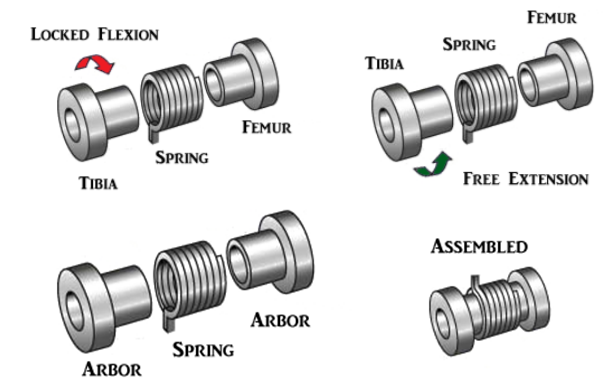
\includegraphics[scale=0.45]{images/mech_design/wrapspringclutch.png}
    \caption[Wrap Spring Clutch]{Wrap Spring Clutch \cite{irby1999optimization}}
    \label{fig:WrapSpringClutch}
\end{figure}


The knee joint for LARRE uses a wrap spring clutch/brake mechanism. \autoref{fig:kneemechASM} shows the knee casing and components.  \autoref{fig:subknee} shows the primary knee mechanism and all the components that comprise the sub-assemblies. The brake engages to lock the knee joint during the stance phase to prevent possible knee flexion and release during the swing phase. The knee's joint consists of a central shaft over which the arbor was mounted via a set screw. The spring wraps around this setup to produce the clutching/braking effect. One end of the spring clamped between the end cover and thigh link, which held the spring in place. A potentiometer is connected to the center shaft to measure joint angles during walking gait.


\begin{figure}
    \begin{subfigure}{\textwidth}
        \centering
        \captionsetup{justification=centering}
        \centerline{
        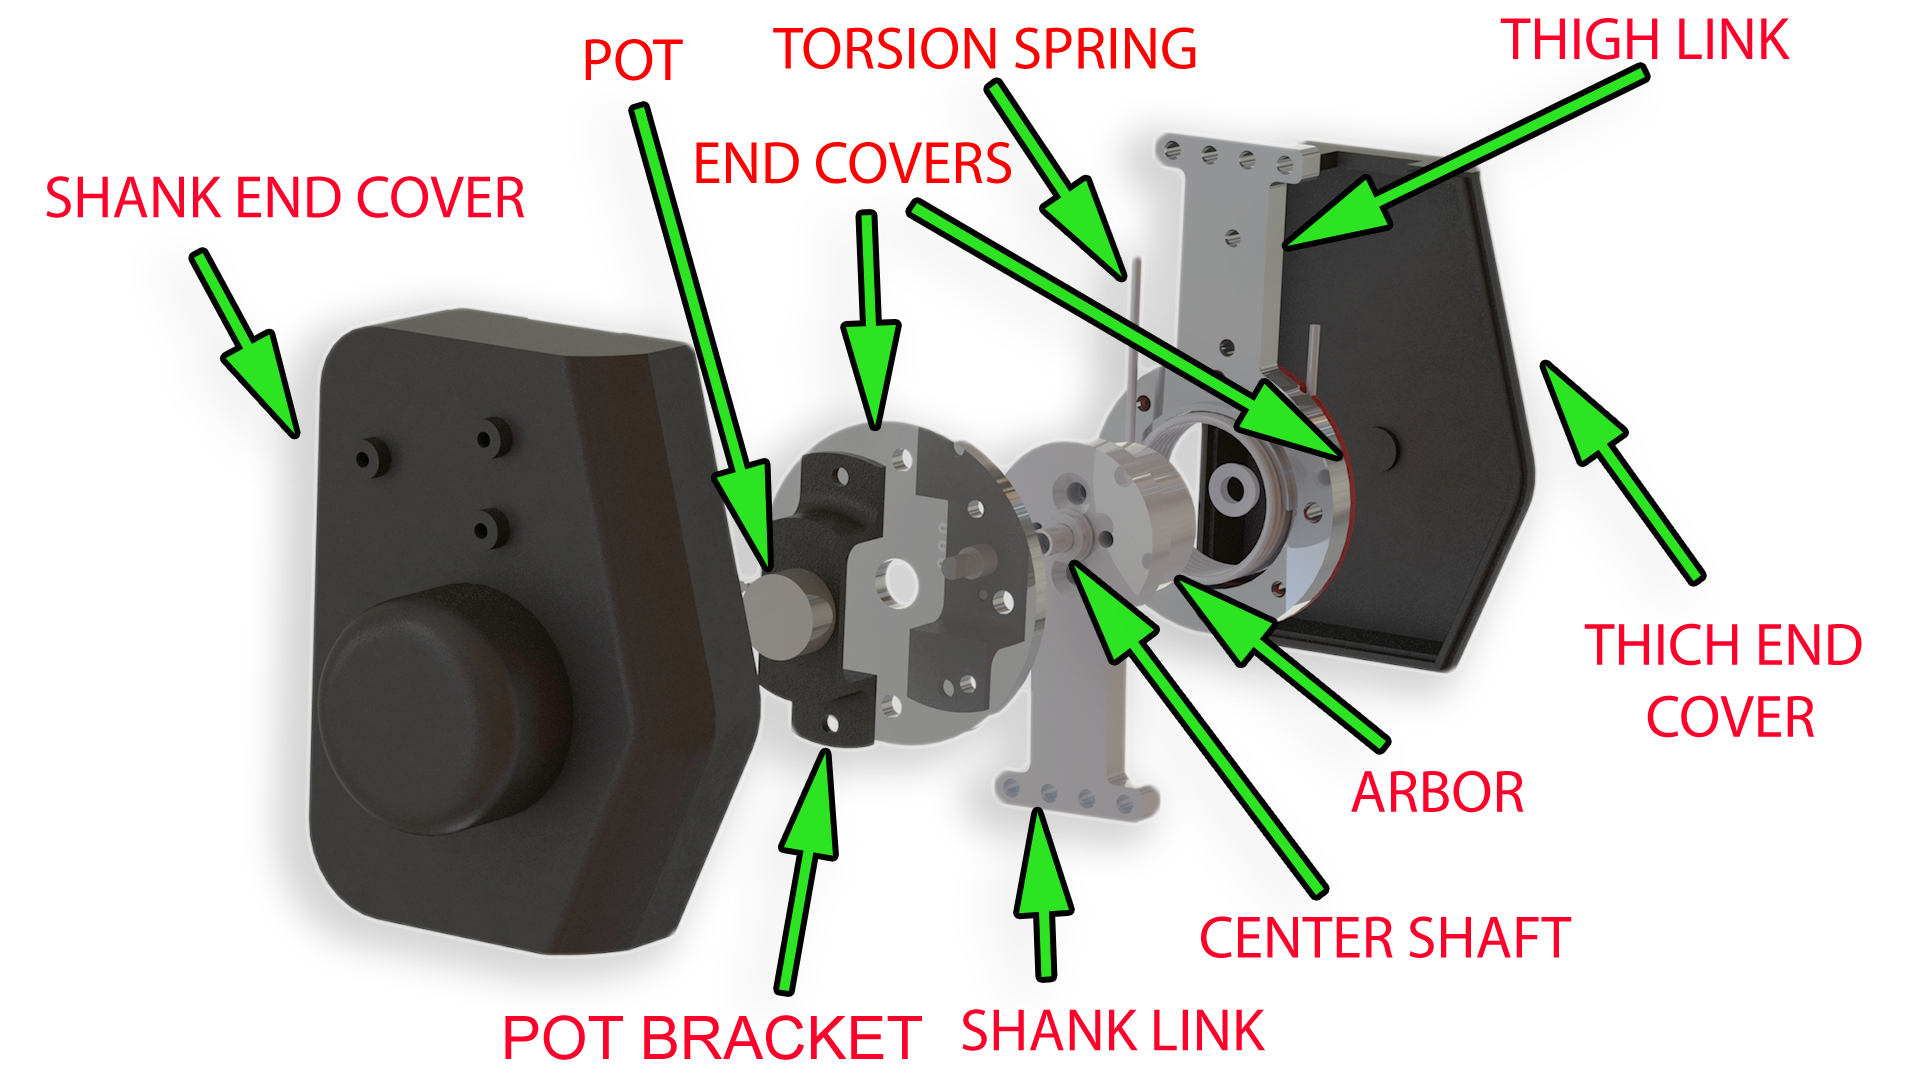
\includegraphics[scale=0.16]{images/mech_design/knee exploded view_edit2.png}}
        \caption[Custom Knee Mechanism]{The custom clutch/brake knee mechanism}
        \label{fig:kneemechASM}
    \end{subfigure}
    \begin{subfigure}{\textwidth}
        \centering
        \captionsetup{justification=centering}
        \centerline{
        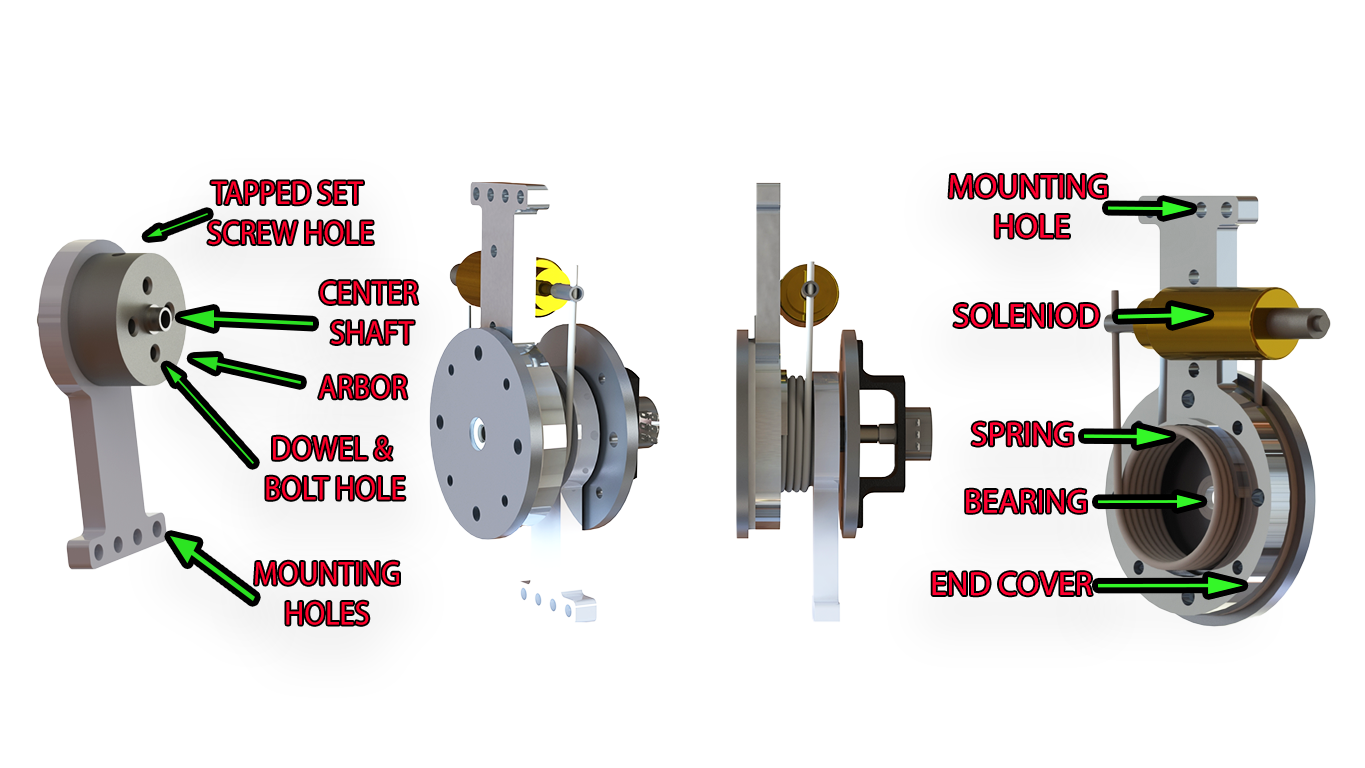
\includegraphics[scale=0.3]{images/mech_design/all_knee.png}}
        \caption[Wrap Spring Clutch Mechanism]{Wrap Spring Clutch Mechanism Sub Assemblies}
        \label{fig:subknee}
    \end{subfigure}    
    \caption{Exloded view of wrap spring clutch knee mechanism}
    \label{fig:kneemech}
\end{figure}

A similar approach represented in \cite{tung2013design} was followed to estimate the arbor diameter and the diametric interference for the design, which is the crucial part of the knee joint. The critical parameters of the knee were measured and summarized in \autoref{tab:KneeDesign}.

\begin{table}[h!]
\centering
 \begin{tabular}{|c || c|} 
 \hline
 Parameter & Value  \\ [0.5ex] 
 \hline\hline
 Spring Coil Inner Diameter   & $43.58132mm$ ($1.7158in$)   \\
\hline
Spring Wire Diameters &   $2.921mm$  ($0.115in$)  \\
\hline
Number of Turns     &   $6.5$ \\
\hline
Diametric Interference    &   $0.70358mm$ ($0.0277in$) \\
 \hline
  Arbor Diameter &  $44.2849mm$ ($1.7435 in$) \\ [1ex]
 \hline
 \end{tabular}
\caption[Knee Parameters]{Knee Design Parameters}
\label{tab:KneeDesign}
\end{table}


% \begin{tabular}{ |c||c| }
%  \hline
%  \multicolumn{2}{|c|}{Knee parameters} \\
%  \hline
% Spring Coil Inner Diameter   & $43.58132mm$ ($1.7158in$)   \\
% Spring Wire Diameters &   $2.921mm$  ($0.115in$)  \\
% Number of Turns     &   $6.5$ \\
% Diametric Interference    &   $0.70358mm$ ($0.0277in$) \\
%   Arbor Diameter (Spring Coil Inner Diameter + diametric interference) &  $44.2849mm$ ($1.7435 in$) \\
%  \hline
% \end{tabular}


% \noindent
% \begin{itemize}
% \item Spring Coil Inner Diameter: $43.58132mm$ ($1.7158in$)
% \item Spring Wire Diameter: $2.921mm$  ($0.115in$)
% \item Number of turns: $6.5$
% \item diametric interference: $0.70358mm$ ($0.0277in$)
% \item Arbor Diameter (Spring Coil Inner Diameter + diametric interference): $44.2849mm$ ($1.7435 in$)
% \end{itemize}


The arbor's initial design had a larger diameter than the spring's inner diameter to establish an interference between the spring and the arbor. This interference creates an initial contact pressure, and when the arbor starts to rotate, the frictional force starts to increase. \autoref{eq:forces}  calculates the average and tangential forces across this region. The Normal and Tangential Forces are used to calculate the holding torque.

\begin{equation}
\large
\begin{aligned}
    \large
    F = pbrd\Phi + p_cbrd\Phi && \text{Normal Force}&\\
    p  = p_0 e^{\mu\Phi} && \text{ Result from Tangential Force}&
    \end{aligned}
\caption[Force Equations for Arbor]{Force Equations}
\label{eq:forces}
\end{equation}

where,
$p$ = total pressure 

$b$ = breadth of the wire 

$r$ = radius of the arbor 

$p_c$ = Centrifugal pressure 

$p_0$ = Initial pressure 

$\mu$ = Frictional coefficient

$d\Phi$ = small angle 

$\phi$ = total angle \\

During midstance, the relative motion between the shank and thigh links in the direction of knee flexion, causing the spring to wrap around the arbor, which produces the wrapping effect. During this condition, the movement between the segments is locked, thus transferring the load to the ground. The brake has to be disengaged to allow free movement during the swing phase, and this is achieved using a linear actuator where the end of the actuator is connected to the spring's free leg. Thus by energizing the actuator, the spring can be unwound. This unwrapping effect of the spring disengages the brake and allows for free knee movement. This normally-closed brake ensures user safety during power failures, and its quasi-passive nature helps sustain the battery for longer cycles of gait. 

Several experiments were conducted in simulation and on the physical model to measure the knee's mechanical properties. The objective of the experiments was to document the properties and limitations of the wrap spring clutch knee. In \cite{SubraMani2020} the experiments are expanded in greater detail. 

A test bed was designed to evaluate the braking torque characteristics and study the relationship between interference and contact forces. A potentiometer was used to measure the knee angle change and a load cell to evaluate the applied load. Based on the collected data, the holding torque of the knee was estimated.

The extension test bed shown in \autoref{fig:Extent_test_bed} was designed to study the frictional force behavior in the knee extension direction. The force on the shank link increased by adding additional mass until the clutch slipped. The point that the system slipped is referred to as the deflection point.

% \begin{figure}
% {images/mech_design/extension_set_up.png}
%     \caption[Extension Test Bed]{Extension Test Bed}
%     \label{fig:Extent_test_bed}
% \end{figure}

This procedure was carried out for different interference values. The load values were substituted into \autoref{eq:ovTorque} to find the new interference values at which the slipped occurred.
\begin{equation}
    \large
    T_U & = p_0br^2(1 - e^{-N2\pi\mu})
\label{eq:ovTorque}
\end{equation}

The inner diameter of the spring is controlled by applying a force to the spring leg. Which also controls the interference between the arbor and spring. \autoref{fig:extension_test} shows the results of  
five different interference measurements. The black dots are the points of deflections for different spring openings. The $0push$ happens when the free spring leg is at its initial $0$ position. $1push$ happens when the spring leg is moved horizontally by a distance of $.313 in$ until $4push$.   

\begin{figure}[h!]
    \centering
    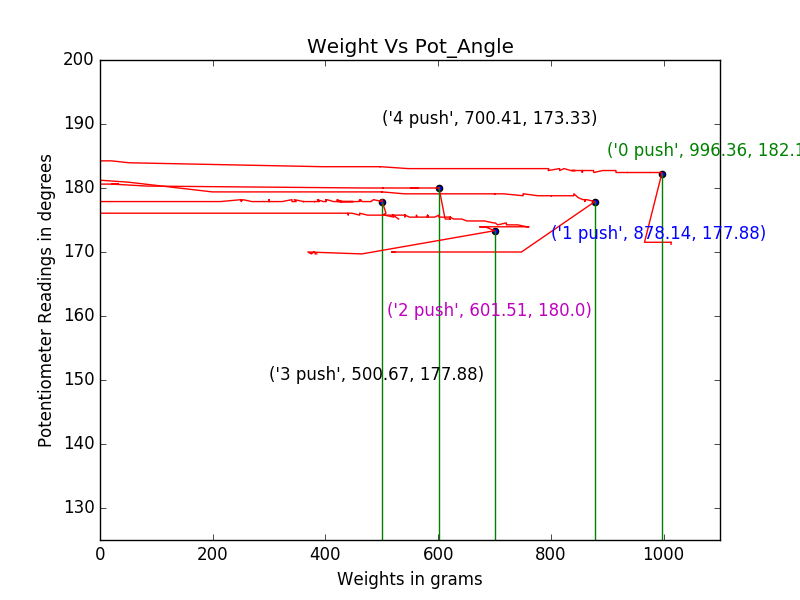
\includegraphics[scale=0.5]{images/mech_design/weighvspot.png}
    \caption[Knee Slipping Load Values]{Slipping Load values during Extension Test}
    \label{fig:extension_test}
\end{figure} 


\autoref{fig:Flexion_test_bed} shows the flexion test bed used to estimate the static and dynamic holding torque behavior of the knee joint. The load applied direction, and the knee flexion direction was along the direction of gravity. The load on the knee was applied at a distance of $0.46m$ from the knee center. The load was applied over several days to measure the durability of the system. This test bed was utilized to find RoM and the brake release force.



\begin{figure}[h]
    \centering
    \includegraphics[scale=0.15]{images/mech_design/flexion_set_up.png}
    \caption[Flexion Test Bed]{Flexion Test Bed}
    \label{fig:Flexion_test_bed}
\end{figure}

The knee was loaded until the knee began to slip. The knee was found to have a maximum holding torque of $63Nm$, after which the knee started to slip. The knee was constructed to hold for an extended period of time, after which the knee lost 4$^{\circ}$ was observed, which was due to excessive stressing on the spring during maximum holding torque. The stress on the spring moved past its elastic region and entered the plastic region, due to which it was not able to coil back to its original position. \autoref{fig:loss_in_rom} shows the result of loss in the range of motion tests.
\begin{figure}[h!]
    \centering
    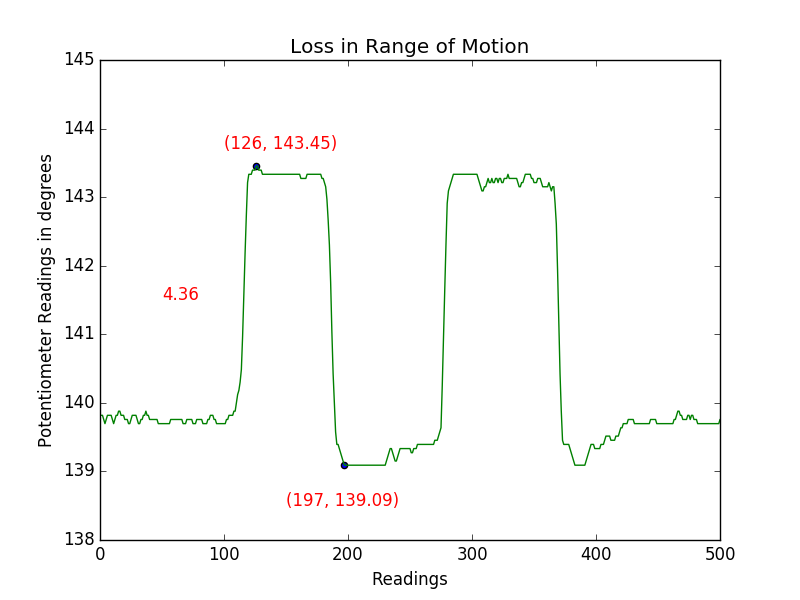
\includegraphics[scale=0.5]{ images/mech_design/loss_in_rom.png}
    \caption{Loss in Range of Motion}
    \label{fig:loss_in_rom}

\end{figure}

\autoref{fig:durabilitytest} shows the results of the durability test. During the test, the brake was engaged at three different loading conditions $48Nm$, $50Nm$, and $63Nm$. The brake was engaged to hold this position for four consecutive days, where the load between the days were increased; $48Nm$ on the first day, $50Nm$ for the second and third (since being the target requirement), and on the fourth day, we pushed the brake to the peak value of $63Nm$. The noise of the sensors was removed using a moving average filter.  The observed angular difference of the brake from the start of the test to the end was $0.75^{\circ}$.

\begin{figure}[h!]
    \centering
    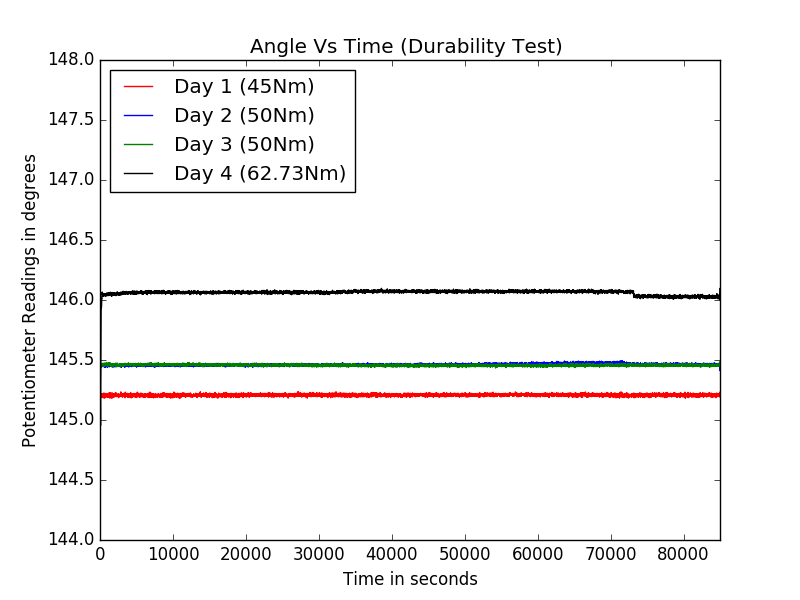
\includegraphics[scale=0.50]{images/mech_design/Durability_test.png}
    \caption{Durability Test}
    \label{fig:durabilitytest}
\end{figure}


The testing results demonstrated that it is possible to build an analytical-based design approach for an actuator using biomechanical and predefined specifications.


The wrap spring clutch knee used an analytical-based design approach for the actuator selection. The knee developed for the LARRE is inexpensive and weighs less than  $1kg$. The system can be easily serviced or repaired. The detailed analytical model was used to identify the relationship between the parameters manipulated to improve the system's overall performance. The wrap spring clutch/brake mechanism underwent a wide range of testing to measure all the necessary knee joint characteristics. 

% \begin{figure}
% \centering
%      \begin{subfigure}{.45\textwidth}
%         \centering
%           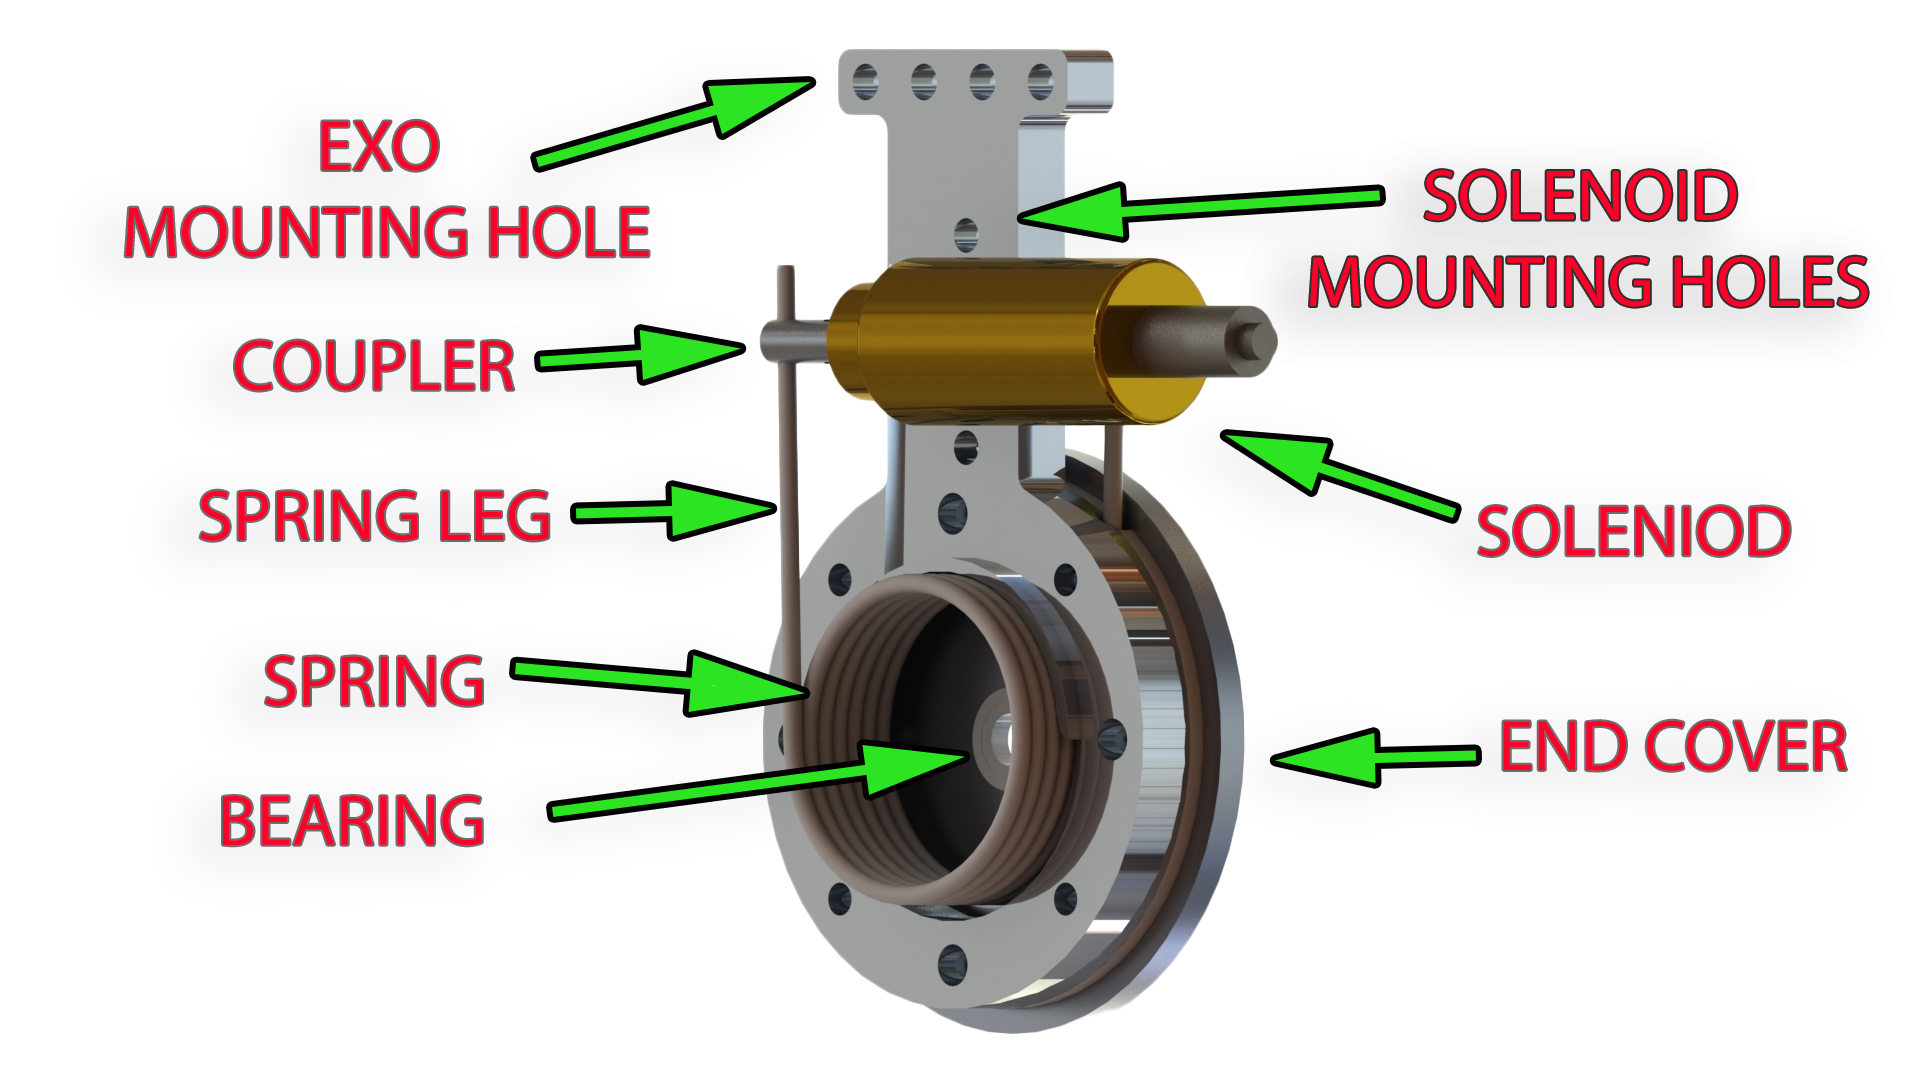
\includegraphics[ scale=0.10]{images/mech_design/thigh_assembly2.png}
%     \caption[Thigh Sub-Assembly]{Thigh Sub-assembly: all components are labeled. The solenoid controls the activation of the brake.}
%     \label{fig:thigh_sub}
%     \end{subfigure} 
%     %
%      \begin{subfigure}{.45\textwidth}
%         \centering
%         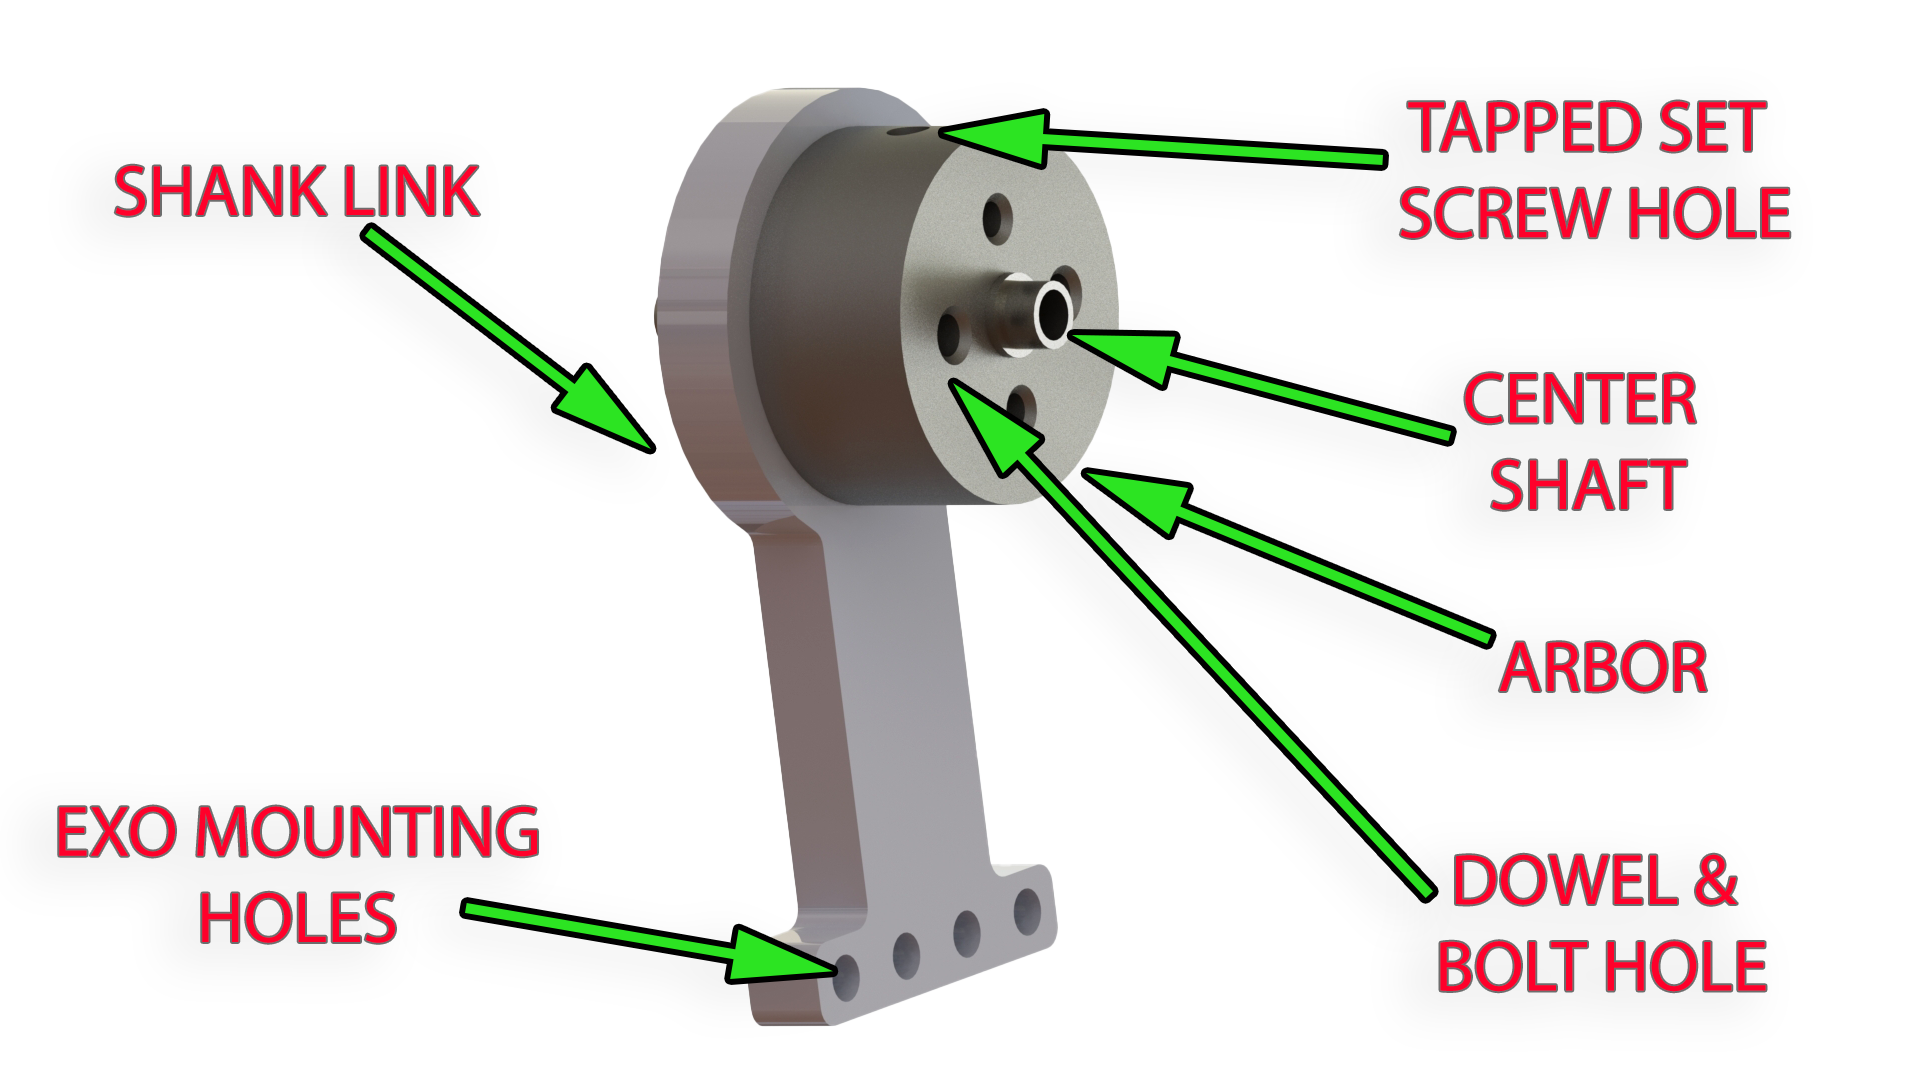
\includegraphics[ scale=0.10]{images/mech_design/shank_assembly2.png}
%         \caption[Shank Sub-Assembly]{Shank Sub-assembly: The arbor interfaces with the spring. When the spring closes, it grabs the arbor and prevents rotation.}
%         \label{fig:shank_sub}
%     \end{subfigure}
%     \caption[Knee Sub-Assemblies]{The Knee sub-assemblies}
%     \label{fig:sub_knee}
% \end{figure}

\section{Prototype of personalized bio-mechanical knee}

The work done in this section was in collaboration with Alex Tacescu \cite{tacescu2021development} and presented at International Mechanical Engineering Congress 2021 [WAITING FOR CITATION]. I led and managed the focus of the project and came up with the idea. I was also involved with running the mocap experiments and the mechanical design. Another knee design was examined that focused on matching the knee motion profile to a human knee. Exoskeletons discussed in \autoref{sec:ExoBack} commonly use pin-type joints in their knee joints; this is in contrast to how the actual kinematics work in a human knew, which has a variable center of rotation \cite{morrison1970mechanics} \cite{koo2008knee}.  This is illustrated by examining MRI scans of knee which show that the femur and tibia have oblong heads\cite{MRIKneeScan}. This geometry translates the tibia as the knee rotates. 


\begin{figure}[h!]
    \centering
    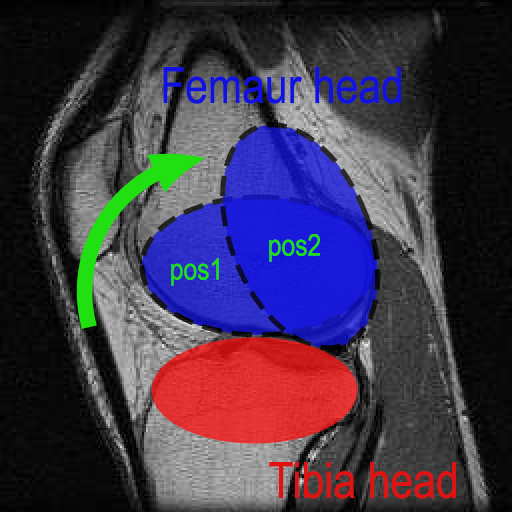
\includegraphics[scale=0.5]{images/mech_design/High-resolution-knee-scan-Resolution-is-025x025x15mm.png}
    \caption[Labled MRI of knee]{MRI of knee the blue oval is the femur head and the red is the tibia head. as the knee rotates the shape of the femur head causes translate of the tibia. As shown in the two position of the femur head.}
    \label{fig:MRIKnee}
\end{figure}

Several recent designs have focused more on accounting for knee motion. Choi \textit{et. al} used multiple rolling cams to adapt to the changing center of rotation \cite{choi2017development}. This design fits a person's knee motion; it did not use modeling of the knee's tibiofemoral motion to design the cams. Additionally, the design is complicated and not easily reproducible. In another design Choi \textit{et. al} used multiple rollers and pulleys powered by electric linear actuators. However, rotary electric motors with rotary gearboxes can often achieve higher performance than electric linear actuators powered by rotary DC motors. Another knee design was presented in \cite{wang2018comfort}; this design prioritized the comfort of the user and the alignment of the knee joint. This design also uses pulleys and cables to model the knee motion. \cite{AdaptiveKneeJoint} presents a cam knee design that uses a model of the knee motion. This design is a significant improvement over previous designs that merely compensate for the motion. However, as the other designs discussed, they use linear actuators.  These designs do well at either mimicking or compensating for the knee motion; however, they are mechanically cumbersome to manufacture; they did not show mimicking of the center of rotation's theoretical movement and/or use a linear actuator to replicate rotary motion. In addition, the design does not allow for the knee to be customized and therefore cannot meet the specific motion of the patient. Thus, we propose a knee design that is readily configured to match a particular patient's knee joint motion, is designed for easy manufacturing, and allows the use of readily available rotary actuators and brake mechanisms.

The variable center of rotation was found using previous work by Iwaki \textit{et. al} that used Magnetic Resonance Imaging (MRI) scans to determine and predict the knee's trajectory \cite{MRIKneeShape_Loaded, MRIKneeShape_Unloaded}. These studies used cadavers and actual patients to measure the motion of the knee in both loaded and unloaded scenarios. This MRI data was used in \cite{KinDynKneeJoint} to build a mathematical model of knee motion that considers both the flexion and extension degrees of freedom. They used ellipse to model the contact between the femur and tibia bones. Their work leads to the formulation of \autoref{eq:KneeExtensionFlexionNumeric}. This equation relates the rotation (in radians) of the knee to the translation of the tibia. In these equation $a$ is a scaling factor and $d$ is an initial offset \cite{wang2013adaptive}. Both of these values are patient specific and can be found using an MRI or motion capture study. \autoref{fig:a_varying} shows the effect of varying the scaling parameters.  This motion and its derivative are shown in \autoref{fig:FlexExtRelationship}. This study was limited since it was based on the anthropomorphic parameters of a single person. These coefficients will vary slightly from person to person and can be found using MRIs or motion capture. 


\begin{equation}
    r(\theta) mm = a(1.08\theta^4 - 11.18\theta^3 + 26.52\theta^2 - 0.825\theta) + d
    \label{eq:KneeExtensionFlexionNumeric}
\end{equation}


\begin{figure}
    \centering
    \includegraphics[width=\columnwidth]{images/mech_design/scalar_varying_a_Annotated.png}
    \caption[Scaling Parameter]{Varying the scaling parameter in \autoref{eq:KneeExtensionFlexionNumeric}[THIS IMAGE NEED TO BE FIXED!!] }
    \label{fig:a_varying}
\end{figure}

% \begin{figure}[ht!]
%     \centering
%     \includegraphics[scale=0.9]{images/mech_design/FlexionCurve.png}
%     \caption{Knee Flexion Curve}{Graphical representation of \autoref{eq:KneeExtensionFlexionNumeric} demonstrating the relationship between flexion and extension in a knee as measured by \cite{KinDynKneeJoint}. \(r(m)\) is the extension distance between the center of the knee and the center of mass of the lower leg. $0^\circ$ represents a perfectly extended knee joint.}
%     \label{fig:FlexExtRelationship}
% \end{figure} 


\begin{figure}[ht!]
    \centering
    \includegraphics[scale=0.9]{images/mech_design/knee_plate_main_annotated.png}
    \caption{Knee Flexion Curve}{Graphical representation of \autoref{eq:KneeExtensionFlexionNumeric} demonstrating the relationship between flexion and extension in a knee as measured by \cite{KinDynKneeJoint}. \(r(m)\) is the extension distance between the center of the knee and the center of mass of the lower leg. $0^\circ$ represents a perfectly extended knee joint. The curve effects the shape of the red cam on the knee plate. }
    \label{fig:FlexExtRelationship}
\end{figure} 

A cam-type mechanism with a brushless DC motor was designed to follow the desired path. The guide was generated using \autoref{eq:KneeExtensionFlexionNumeric}. This guide enforces variable center of rotation and motion of the tibia. \autoref{fig:ExplodedViewLabeled} shows an exploded view of the knee mechanism. 



\begin{figure}
    \begin{subfigure}{\textwidth}
        \centering
        \captionsetup{justification=centering}
        \includegraphics[scale=0.2]{images/mech_design/ExoKneeExplodedView.png}
        \caption{Bio Knee joint design exploded view}{Knee joint design exploded view}
        \label{fig:ExplodedViewLabeled}
    \end{subfigure}
    \begin{subfigure}{\textwidth}
        \centering
         \includegraphics[scale=0.2]{images/mech_design/KneeJointAssyCrossSection.png}
          \captionsetup{justification=centering}
        \caption{Cross section of Bio knee}{A cross section of the knee joint with the potentiometer embedded in the design. The wires are routed along the wire channel to avoid interference with the inner arm and plastic slides}
        \label{fig:CrossSectionPot}
    \end{subfigure}    
    \caption{Exploded View of bio-knee mechanism}
    \label{fig:bioknee}
\end{figure}

The motor and gearbox need to provide sufficient torque and power to drive the knee of a $100kg$ patient through gait motion. This mass is larger than the average mass of the North American paraplegic, which is $68.8kg$, so assuming a larger mass allows for the motor to have a safety factor. Additionally, it is assumed that the dynamic loads are assumed to be negligible during the slow-motion collision with the ground. It equates to approximately $65W$ of power and $25Nm$ of torque at \(15^\circ/sec\). The knee is powered by a $90W$ brushless Maxon motor used with a nominal torque of $0.56Nm$ at roughly $2500rpm$.  The motor is combined with a Harmonic gearbox with a $100:1$ reduction. \autoref{table:MotorGearboxSpecs} shows the gearbox and motor specifications and the joint's mechanical properties. The calculations assumed an efficiency of \(90\%\) as per the manufacturer documentation. The designed knee joint can mechanically output $81W$ and $50.4Nm$ at $15^\circ/sec$.  

\begin{table}
    \centering
    \begin{tabular}{||c|c|c||}
        \hline
        Input (Motor) Power & \(P_{input}\) & \(90 Watts\) \\
        \hline
        Input (Motor) Torque @ Nominal & \(\tau_{input}\) & \(0.560 Nm\) \\
        \hline
        Input (Motor) Speed @ Nominal & \(\omega_{input}\) & \(2510 rpm\) \\
        \hline
        Input (Motor) Stall Torque & \(\tau_{in\_stall}\) & \(7.480 Nm\) \\
        \hline \hline
        Gearbox Ratio & \(\frac{n_1}{n_2}\) & \(100:1\) \\
        \hline \hline
        Output Power & \(P_{output}\) & \(81 Watts\) \\
        \hline
        Output Torque @ Nominal & \(\tau_{input}\) & \(50.4 Nm\) \\
        \hline
        Output Speed @ Nominal & \(\omega_{input}\) & \(15^\circ/sec\) \\
        \hline
        Output Stall Torque & \(\tau_{out\_stall}\) & \(673.2 Nm\) \\
        \hline
    \end{tabular}
    \caption{Bio Knee parameters}{Motor/gearbox specifications and output power specifications of the proposed joint.}
    \label{table:MotorGearboxSpecs}
\end{table}

The design was validated using a motion capture system and SolidWorks motion analysis \footnote{https://www.solidworks.com/category/simulation-solutions}. The markers on the knee were aligned on the shank and thigh segments of the knee and rotated through the desired motion as shown in \autoref{fig:KneeJointTestSetup}; this allowed us to compare the theoretical trajectory to the actual trajectory, and for the measurement and comparison of manufacturing tolerance. \autoref{fig:KneeJointTestResults} shows the results of the study. There are some slight deviations of the actual motion compared to the desired motion; this deviation is caused by hysteresis in the system. However, these movements are very slight on a scale of less than $1mm$, which is assumed to be negligible.   



\begin{figure}[ht!]
    \centering
    \includegraphics[scale=0.07]{images/mech_design/KneeTrajTest_edit.png}
    \caption{Knee with mocap markers}{Knee joint setup with motion capture dots}
    \label{fig:KneeJointTestSetup}
\end{figure}

\begin{figure}[ht!]
    \centering
    \includegraphics[scale=0.75]{images/mech_design/FlexionExtensionKneeJoint.png}
    \caption{Comparison of variable center of rotation}{Graph showing knee joint flexion vs linear extension of the radius of curvature for the goal trajectory (see \autoref{eq:KneeExtensionFlexionNumeric}) and the experimental results from the Motion Capture Study}
    \label{fig:KneeJointTestResults}
\end{figure}


The presented prototype of the knee joint can move through the desired joint range and replicate the tibiofemoral path of a biological knee. \autoref{fig:LARRE_KneeJoint_Render} shows the presented knee in the rendering of LARRE. The motor produces the required torque, and the potentiometer and encoder in the motor allow for feedback control. The use of FEA showed that the knee could withstand the anticipated forces without structurally failing. These tests are necessary for ensuring that the knee can withstand force. The knee is a key joint for maintaining upright posture and preventing falling. If the knee joint fails during operation the patient could fall and be injured. 

A key part of the design was ensuring that the system could be easily manufactured and customized. All of the parts are can be manufactured with minimal manufacturing experience. All of the custom components are 3D printable on inexpensive consumer-grade 3D printers with consumer-grade PLA filament. The other components are off-the-shelf components. The presented design is ideal for customization and manufacturing. The presented knee was designed to follow a previously established trajectory. Additional testing needs to be conducted to identify the patient-specific parameters so that the polynomial can be fitted to the individual. Using MRI images of the femur and tibia heads or potential using motion capture to measure the translation and rotation of the tibia relative to the femur, this work is currently ongoing. 

\begin{figure}
    \centering
    \includegraphics[scale=0.15]{images/mech_design/exo_with_bioknee.png}
    \caption[Rendering of LARRE with the Bio-Knee]{A Rendering of LARRE with the Bio-knee}
    \label{fig:LARRBio-Knee}
\end{figure}




\section{Ankle Foot Orthosis}
\label{sec:ankle}
The work done in this section was in collaboration with Nathaniel Michaels \cite{michaels2020modular}. I was the lead designer and gave feedback for the mechanical and electrical design. I also designed and helped run the experiments for the validation of the systems. 

The ankle-foot orthosis (AFO) of LARRE comprises two components, a passive ankle joint to keep the foot straight and a sensor to sense the ground force reactions. The design process of the AFO is discussed in more detail here \cite{Michaels2020}.  A rendering of the AFO mechanism is shown in \autoref{fig:AFO Mechanism Full} and \autoref{fig:Outer Ankle Box fig}. The AFO is designed to fit over the shoe to allow the operator to easily donn and doff the exoskeleton, uses a passive spring to balance the foot's mass and prevent foot drop while still allowing flexion, and the sensing sole detects the phases of the gait cycle. 

\begin{figure}[h!]
    \centering
    \begin{subfigure}[b]{0.45\textwidth}
        \centering
        \captionsetup{justification=centering}
        \centerline{
        \includegraphics[scale=0.2]{images/mech_design/AFO_Exploded_AND_Force_Sole_WITH_Labels2.png}}
        \caption{AFO Mechanism. There are three parts to the system; the outer ankle box, the sensing sole, and the the metal foot plate}
        \label{fig:AFO Mechanism Full}
    \end{subfigure}
    %
    \begin{subfigure}[b]{.45\textwidth}
        \centering
        \captionsetup{justification=centering}
        \centerline{
        \includegraphics[scale=0.15]{images/mech_design/Outer_Ankle_Box_Exploded_WITH_Labels2.png}}
        \caption{Outer Ankle Box Exploded View. This system transfers the body load from the legs to the floor. The spring }
        \label{fig:Outer Ankle Box fig}
    \end{subfigure}%
    \caption{AFO Sub-Assemblies}
    \label{fig:AFO Sub-Assemblies}
\end{figure}


The sensing sole has Ohmite FSR03C3 Force Sensing Resistors (FSRs) \footnote{https://www.ohmite.com/catalog/fsr-series/FSR03CE} embedded into the toe and heel areas of the sole. FSRs are flat flexible resistors that change their electrical resistance based on the applied force \cite{yaniger1991force} and convert the force to an electrical signal by measuring the sensor's variation of conductivity. The small flexible forum factor force-sensing makes them ideal sensors for wearable devices \cite{giovanelli2016force}.    

FSRs embedded into the sole of an AFO can measure the gait phases. Patar \textit{et. al} two embedded FSRs into their AFO to measure the transition pressure points in the foot during the gait cycle\cite{ab2014system}. In their model, a single FSR was placed on the foot's heel and ball, respectively.  

\autoref{fig:SensingSole} shows the sensors' locations and the sensors connected to LARRE. The FSRs are encased in a Urethane risen. The risen distributes the ground forces onto the sole and protects the sensors from being damaged. The resin has properties similar to shoes' soles, with a shore hardness of 20 and a non-stick surface \footnote{Vytaflex20Website}. Both Vytaflex-20 \footnote{https://www.smooth-on.com/products/vytaflex-20/} and Vytaflex-30 \footnote{https://www.smooth-on.com/products/vytaflex-30/} were tested as possible options. Once the system was cured, the Vytaflex-30 material had a sticky surface texture. It was not suitable since contact with the ground and dirt and debris would stick to the surface. The Vytaflex-20 material was cured with a surface and was much less sticky, making it better than the Vytaflex-30 material for encasing the sole sensors. 

The Vicon motion capture system and the AMTI force plates were used to measure the center of pressure of the AFO.  The measurement was used to detect the individual reading of the FSR and to validate the AFO's CoP. Each of the FSR's was treated as an on-off switch. If the pressure detected was above a threshold, it was treated as "on," below the threshold as "off."  Several different versions of the AFO were tested; the final version of the sensors readings and filtering is shown in \autoref{fig:FSRBinarized}. As shown, the filtering removes the noise from the sensor reading. \autoref{tab:statetable} shows a state table to detect the different states of the AFO. 

\begin{figure}[h!]
    \centering
    \includegraphics[scale=0.45]{images/mech_design/SoleSensorV3T2_Raw_v_Binarized.png}
    \caption[Measurement of raw FSR]{Measurement of raw FSR activation and filtering \cite{Michaels2020}}
    \label{fig:FSRBinarized}
\end{figure}


\begin{table}[h!]
    \centering
    \begin{tabular}{|c|c|c|c|}
    \hline
    FSR1 - Inner Ball & FSR2 - Outer Ball & FSR3 - Heel & Position-State \\[0.5ex]
    \hline\hline
    0 & 0 & 0 & Foot not on ground \\
    \hline
    0 & 0 & 1 & Heel-Down \\
    \hline
    0 & 1 & 0 & Transition or Error \\
    \hline
    0 & 1 & 1 & Leaning Outward \\
    \hline
    1 & 0 & 0 & Transition or Error \\
    \hline
    1 & 0 & 1 & Leaning Inward \\
    \hline
    1 & 1 & 0 & Toe-Down \\
    \hline
    1 & 1 & 1 & Flat-Foot \\
    \hline
    \end{tabular}
    \caption[AFO State Table]{AFO Position State-Table with FSRs as bits \cite{Michaels2020}}
    \label{tab:statetable}
\end{table}



% \begin{figure}[h!]
%     \centering
%     \includegraphics[scale=0.25, angle =-90 , frame]{images/mech_design/sole.png}
%     \caption[Pressure Map of Foot]{Overlay of Pressure Map with current Foot Sensor design \cite{michaels2020modular}}
%     \label{fig:Foot-Force Mapping}
% \end{figure}

\begin{figure}[h!]
    \centering
    \includegraphics[scale=0.08]{images/mech_design/SoleSensor_in_Footplate.png}
    \caption[Sensing Sole]{Sensor Sole in LARRE. The FSR are embedded in the Vytaflex resine.}
    \label{fig:SensingSole}
\end{figure}



Finite element analysis (FEA) was used to validate that the AFO could withstand the applied forces \cite{akin2010finite}. The FEA analysis was conducted using SolidWorks \footnote{https://www.solidworks.com/} FEA tools; this allowed for each of the individual components to be tested and validated before being manufactured. The testing showed that components under the assumed loads, the Von Mises \cite{shigley} stress, did not exceed the materials' yield strength and would not break.

\begin{equation}
\large
    \{x,y\}_{cop} = \sum_{i}^{N} \{x,y\}_i F_i
    \label{eq:FSRCoP}
\end{equation}

The Center of Pressure (CoP) of the AFO is measured by using \autoref{eq:FSRCoP}, where $\{x,y\}$ is the location of the FSR and $F$ is the force of the FSR. The location of FSRs is shown in \autoref{fig:AFOmocap}. The CoP was validated using the mocap and force plates. The force was measured using the force plate, which provides the force along each axis, and the mocap markers located the force vectors in space. The mocap+forceplates were used to dead reckon the FSR sensors. 




 \begin{figure}[h!]
    \ContinuedFloat
           \captionsetup{justification=centering}
           \centerline{ \includegraphics[scale=0.25]{images/mech_design/Mocap_Layout_2.png}}
            \caption[AFO Mocap Markers]{Location of mocap markers and FSRs on the AFO \cite{Michaels2020}}
            \label{fig:AFOmocap}
    \end{figure}


The results of the CoP measurement are summarized in \autoref{fig:3DFSRCoP} and \autoref{fig:FSRCoPAFO}. The shape created by the AFO point shows major distortions across the $x$ axis compared to the force plate. The $z$ axis can be ignored since it is perpendicular to the page and has no significant meaning. The major axis of interest is the $y$ axis that goes along the foot's cardinal longitudinal axis. These FSRs can track the CoP measured by the force plates. 


\begin{figure}[h!]
    \centering
    \begin{subfigure}{0.5\linewidth}
        \captionsetup{justification=centering}
        \centerline{ \includegraphics[scale=0.35]{images/mech_design/SoleSensorV3_CoPComparison_2D_XYplane.png}}
        \caption[CoP comparison]{The CoP comparison results between the calculated AFO CoP point and the Force-Plate CoP point within the world frame, across both trials.}
        \label{fig:3DFSRCoP}
    \end{subfigure}%
    \vspace{1cm}
    \begin{subfigure}{.5\linewidth}
        \captionsetup{justification=centering}
        \centerline{\includegraphics[scale=0.35]{images/mech_design/SoleSensorV3_CoPComparison_BothTrials.png}}
        \caption[CoP Point Trail ]{CoP Point trail created by both the Force-Plates and AFO across both trials. }
        \label{fig:FSRCoPAFO}
    \end{subfigure}%
    \caption[Center of Pressure of the AFO]{Center of pressure of the AFO measured using the FSRs compared to the forceplate measurement \cite{Michaels2020}}
    \label{fig:CoPAFO}
\end{figure}


This device combined passive-dorsiflexion control methods and sensory feedback systems into a single AFO device for LARRE. This device acts as a fully-functional DAFO device capable of controlling foot-drop using a passive torsional-spring system. The devices provide real-time feedback for balance control and force distribution.  Using three FSRs instead of two makes it possible to determine the CoP point within the support polygon they form.  This information can be used by the main controller onboard the LARRE to help the system maintain its balance.


\section{Final Design}

LARRE's leg segments are constructed from 6061 aluminum alloy concentric sliding pipes with clamps allowing the joints' to be adjusted for each person. This material is lightweight and easy to manufacture. The axles of the joints were constructed of steel to handle the expected stress. Safety is a significant concern; careful attention was given to the manufacturing process to minimize the sharp edges since it is attached to a human-machine interface system. Safety is essential for people with SCI who have minimal sensory abilities and would not feel an injury.  LARRE is attached to a person through the upper body and waist straps. Custom-made 3D printed strap carriages are placed on the thigh and shank segment and connect the person to the exoskeleton's legs. \autoref{fig:LARRE} shows the final model of LARRE.     


\begin{figure}
    \centering
    \includegraphics[scale=0.08]{images/mech_design/exo_side2.png}
    \caption{The LARRE exoskeleton being worn}
    \label{fig:LARRE}
\end{figure}


The dynamic properties of LARRE are essential for building the controller. The dynamics of LARRE were calculated using SolidWorks. The properties account for the material properties of the components as well as the geometry. \autoref{tab:LARREMASS} summarizes the dynamic properties of LARRE. The exoskeleton has defined joint limits to allow for biological motion, summarized in \autoref{tab:jointlimits}.

\begin{table}[h!]
    \centering
    \begin{tabular}{|c c c c c|}  
         \hline 
          \multicolumn{5}{|c|}{Exoskeleton Segment Parameters} \\
         \hline
         Link & Mass (kg) & $CoM_x$ & $CoM_y$ & $CoM_z$ \\
         \hline \hline
         Hip & 2.3677 & 0.000011338 & 0.093937 &  -0.12619 \\
         Thigh & 2.1138 & 0.0034745   & 0.097979 &  0.1712 \\
         Shank & 1.2804  &   0.002761 & 0.097563   & 0.15581\\
         Foot & 0.85523 & 0.14092 & 0.2267 &  -0.31138  \\
         \hline
    \end{tabular}    
    \caption[Dynamic Properties of the LARRE]{Mass Properties of the LARRE}
    \label{tab:LARREMASS}
\end{table}


\begin{table}[h!]
\begin{centering}
    \begin{tabular}{ |p{1cm} p{2cm} p{2cm} |  }
        \hline 
        \multicolumn{3}{|c|}{LARRE Joints Limits} \\
        \hline 
        Joint & Flexion & Extension \\
        \hline \hline
        Hip   & $-60^{\circ}$   & $30^{\circ}$  \\
        Knee &   $-110^{\circ}$  & $0$   \\
        Ankle & $-20^{\circ}$ & $20^{\circ}$  \\
        \hline
    \end{tabular}
    \caption[LARRE Joint Limits]{Joint limits}    \centering
    \label{tab:jointlimits}
\end{centering}
\end{table}


A single patient study was conducted to measure the kinematics and dynamics of a gait while wearing LARRE. This study was not designed to measure the ability of the exoskeleton to induce movement but merely to observe the motion of the exoskeleton. The Vicon setup described in \autoref{sec:setup} was used with the custom marker layout shown in \autoref{fig:larremarker}. Additional markers were added to the plug-in gait model. \autoref{tab:exomarkerlayout} details the rigid bodies used and their location (see \autoref{fig:markers} for definition of the marker layout). The additional markers were added to ensure that there was no marker occlusion during the trial. 

The joint kinematics are shown in \autoref{fig:exojointkin}. Only a single demonstration is shown; however, multiple demonstrations were recorded. Similarly, data were recorded for both legs, but just the right leg is shown. The heel strikes and toe-offs are pointed out in the graphs. These points are calculated using the Vicon plug-in gait tools. All of the data presented were extracted and analyzed using the tools discussed in \autoref{chap:software}. In this study, three steps were taken across the mocap floor. The first step was slightly off since it started with feet together; however, steps two and three aligned with the expected motion. The gait cycles are presented over the collected frames; the Vicon records at 100FPS, so the presented trial is approximately $14.04s$. LARRE was able to move through the desired joint range for a gait cycle. Similarly, with the moments shown in \autoref{fig:larregaitmoments}, the first step did not contain relevant data since the moments can only be calculated when the force plates embedded on the floor are stepped on. The moments are presented in $\frac{Nm}{Kg}$ which allows for the torque to be abstracted and calculated for the different masses. 

\begin{table}[h!]
    \begin{centering}
            \begin{tabular}{||c  c ||} 
         \hline
            Plate Name & Plate \#  \\ [0.5ex] 
            \hline\hline
            LTHIGH	& 11 \\
            LSHANK &	19\\
            LFOOT &	9 \\
            LTHIGH FRONT &	7\\
            LTHIGH BACK &	15\\
            LSHANK FRONT &	4\\
            LSHANK BACK &	14\\
            RTHIGH SIDE &	5\\
            RSHANK SIDE &	17\\
            RFOOT &	10\\
            RTHIGH FRONT &	20\\
            RTHIGH BACK &	16\\
            RSHANK FRONT &	1\\
            RSHANK BACK &	3\\
            BACK &	2\\ [1ex] 
         \hline
        \end{tabular}
        \caption[Exoskeleton Rigid Body Numbers]{Rigid Body Numbers}
        \label{tab:exomarkerlayout}
    \end{centering}
\end{table}




\begin{figure}[h!]
    \begin{subfigure}{0.5\textwidth}
        \centering
        \captionsetup{justification=centering}
        \centerline{
        \includegraphics[scale=0.1, frame]{images/mech_design/exo_markers_back.png}}
        \caption[LARRE marker set back/side]{LARRE marker set back/side}
        \label{fig:larremarkerside}
    \end{subfigure}
    \begin{subfigure}{0.5\textwidth}
        \centering
        \captionsetup{justification=centering}
        \centerline{
        \includegraphics[scale=0.1, frame]{images/mech_design/exo_markers_front.png}}
        \caption[LARRE marker set front]{LARRE marker set front}
        \label{fig:larremarkerfront}
    \end{subfigure}    
    \caption{Marker set for LARRE}
    \label{fig:larremarker}
\end{figure}



\begin{figure}
    \begin{subfigure}{\textwidth}
        \centering
        \captionsetup{justification=centering}
        \centerline{
        \includegraphics[width=\textwidth, frame]{images/mech_design/exo_joint_angles.png}}
        \caption[LARRE gait cycle angles]{Gait cycle angles of the LARRE}
        \label{fig:larregaitangles}
    \end{subfigure}
    \begin{subfigure}{\textwidth}
        \centering
        \captionsetup{justification=centering}
        \centerline{
        \includegraphics[width=\textwidth, frame]{images/mech_design/exo_joint_moments.png}}
        \caption[LARRE gait cycle moments]{Gait cycle moments of the LARRE}
        \label{fig:larregaitmoments}
    \end{subfigure}    
    \caption{Gait cycles kinematics for LARRE}
    \label{fig:exojointkin}
\end{figure}






% \begin{table}[h!]
% \begin{centering}
%     \begin{tabular}{ |p{1cm} p{2cm} p{2cm} p{2cm}|  }
%         \hline 
%         \multicolumn{4}{|c|}{LARRE Joints Limits} \\
%         \hline 
%         Joint & Flexion & Extension & Torque \\
%         \hline \hline
%         Hip   & $-60^{\circ}$   & $30^{\circ}$ &  60N \\
%         Knee &   $-110^{\circ}$  & $0$  & 50N \\
%         Ankle & $-20^{\circ}$ & $20^{\circ}$ &  - \\
%         \hline
%     \end{tabular}
%     \caption[LARRE Joint Limits]{Joint limits}    \centering
%     \label{tab:biomech}
% \end{centering}
% \end{table}



\section{Contributions}

The developed exoskeleton allows for a modular and comprehensive method to test and develop different joints mechanisms. The modular connection interfaces allowed for the development of several different mechanisms. The mechanical design and SolidWorks parts were released open source for the community to use. By providing the basic mechanical structure, researchers can put more effort into constructing new sensors and mechanical actuators instead of the entire system. The platform also allows for adjustment to the user. The legs can be extended to fit the person's legs, and the hip-width can be expanded to ensure a good fit. This feature is critical for testing the exoskeleton on different people. The presented joint designs undergone testing and analysis to show the functionality. The two different knee designed each provide a novel and unique design approach. The wrap spring clutch mechanism is a quasi-passive system that will provide support to the user and prevent buckling. The Bio-knee is fit can be easily manufactured and designed to fit the anthropomorphic parameters of the person. 


\chapter{Generalization of Stair Climbing}

\section{Introduction}
Stair climbing is an important ADL. Exoskeletons need to be able to generate trajectories to climb the stairs. This work focuses on generating the trajectory from the start to the goal, not considering balance and stability. This research is not focused on the dynamics of maintaining upper body stability. It is directed on learning joint trajectories and therefore assumes that the goal point is within the exoskeletons support polygon using zero moment point \cite{kajita2003biped}.


By combining Stair Climbing LfD methods, step motions can be generalized and reproduced. Allowing for demonstrations of a single stair height to generate trajectories for different climbing heights simplifies the training process since all possible step heights cannot be collected for training data. Additionally, since the foot location is used as the training set, it abstracted the leg lengths and thus the person's height, allowing the motion to be reproduced for people of different heights. A similar recording method described in \cite{hicks2011lower} was used as the basis for the study. \autoref{fig:stairoverlay} shows the Vicon image of a person climbing the stairs. The collected data set was generalized with GMM and GMR. This collection and encoding method allowed robust data collection combined with a well-studied framework of teaching lower limb exoskeleton trajectories. Together, these methods allow a compilation of data to generalize a trajectory for stair climbing for people and stairs of different heights. This model shows that there is no need to retrain the trajectory for each person and different stair heights.



\begin{figure}
    \centering
    \includegraphics{images/stairs/mocap_overlay_stairs.jpg}
    \caption[Stair Mocap Overlay]{Subject with Mocap Overlay Climbing the Staircase. The stair case could be adjusted for the different trials by inserting wooden plates that were secured by bolts.}
    \label{fig:stairoverlay}
\end{figure}

\section{Learning of the Trajectories}
This work was published in IEEE Transactions on Medical Robotics and Bionics\cite{goldfarb2021towards}. \autoref{fig:stick} shows the coordinate layout used in this paper. The $X$ axis is perpendicular to the plane and is not considered since the exoskeleton does not have actuation along the $X$ axis. \autoref{fig:stick} shows a diagram of the subject in motion. In this diagram, the toe's position is controlled from the ground to the first step of the staircase. GMM (\autoref{eq:Mstep},\autoref{eq:Estep}) is used to learn the $Z$ and $Y$ marker position. The human demonstration (\autoref{chap:gaitdata}) was paired to find the stepping motion of the subject. Using GMR (\autoref{eq:GMR_Prop}, \autoref{eq:GMR_mu} ) the driving force is calculated. The forcing function is used to drive the model along the trajectory. DMPs (\autoref{eq:DMP_force}, \autoref{eq:DMP_Model} ) are used to replicate and alter the the trajectory to climb stairs of various heights.  


The limb length of the subject used for training was measured using a calibration phase. However, the limb length segments can be estimated using the height of the subject \cite{anthropomorphic}. It is assumed that the relative location of stairs is known with respect to the person. The motion has to be transferred to joint space using inverse kinematics of the leg. To avoid a collision of the toe with the lip of the stairs, a constraint that the foot must be parallel to the ground is imposed. In addition, some rehabilitation exoskeletons do not have actuated ankle joints and therefore cannot be controlled.  \autoref{eq:IK} is the inverse kinematics of the leg with a constrained ankle where hip: $q_1$, knee: $q_2$, ankle: $q_3$, thigh: $l_1$, shank: $l_2$, ankle height: $l_3$, foot length: $l_4$, $z_{toe}$ and $y_{toe}$ is the coordinate of the toe. Inverse kinematics allows for the encoding of the stair height instead of forward kinematics. 

\begin{equation} 
    \begin{aligned} 
        y' &= y_{toe} - l_4 \\ 
        z' &= z_{toe} + l_3 \\  
        \gamma &= y'^2 - z'^2 - l_1^2  - l_2^2 \\ 
        q_2 &= atan2 \Bigg( -\sqrt{1 - \frac{\gamma }{2 l_1^2 l_2^2}}, \frac{\gamma}{2 l_1^2 l_2^2}\Bigg)\\ 
        q_1 &= (atan2(z, y) - atan2( l_2 s_{q_2}, l_1 + l_2 c_{q_2})) + 0.5\pi \\ 
        q_3 &= (2\pi - q_1 - q_2) 
    \end{aligned} 
    \label{eq:IK} 
\end{equation} 

 
\begin{figure} 
    \centering 
    \includegraphics[scale=0.9]{images/stairs/stick.png}
    \caption[Stair Climbing Motion]{Figure representing the stair climbing motion of a 3 DoF leg. The start and goal are the parameters of the model shown as the distance $d$ and height $h$ from the toe to the stair. Each of the joint angles are calculated using inverse kinematics} 
    \label{fig:stick}
\end{figure} 

\autoref{fig:DTWStairs} shows the alignment of a trajectory against a demonstration. This demonstration was taken from stair climbing data set. The blue line is demo 1, and the orange line is demo 2. DTW aligns demo 2 with demo 1. The green line represents the aligned trajectory, and the red line represents a polynomial fit to the aligned trajectory. The cost map shows the closest fit of points from $P$ to $T$. The white spots are the hills, and the black spots are the valleys, with the path being the minimum cost from start to goal. The total path cost associated with the Euclidean was $17652.35$, and the cost of the Manhattan path was $33.50$. These are the costs of aligning the demonstration with the model trajectory. The Manhattan metric had a much lower cost than the Euclidean metric, allowing for a better fit. 

\begin{figure}[h]
     \centering 
     \includegraphics[width=\textwidth]{images/stairs/DTW_annotated.png} 
     \caption[Polynomial Smoothing of DTW]{Two demos being aligned using DTW and a smoothed trajectory. Blue line: demo 1. Orange line: demo 2. Green line: aligned trajectory. Red line: Polynomial smooth trajectory. The cost map shows the distance between the points.} 
     \label{fig:DTWStairs} 
\end{figure} 



The BIC score was used to optimize the number of required bins for the GMM process. \autoref{fig:BIC} shows the BIC score calculated for several bin sizes (1-25) for the $ Y $ and $ Z $ trajectories of the toe marker. This calculation limits the number of bins. The two graphs are generated using a single demonstration from each of the eight subjects in the config0 data set (see \autoref{tab:stairs}). The optimal number of bins for the $Z$ axis is 11 bins, and the optimal number of bins for the $Y$ axis is 14 bins. 


\begin{figure}[h!]
   \begin{subfigure}{\linewidth} 
    \centering 
    \ContinuedFloat
    \includegraphics[ scale=0.6]{images/stairs/ybic7.png}
    \caption[BIC Score for $Y$ Toe]{BIC score for toe marker $Y$ position trajectory. The BIC score has its first local minimum at a size of 14 bins.} 
    \label{fig:BICY} 
  \end{subfigure}  
\begin{subfigure}{\linewidth} 
    \centering 
    \ContinuedFloat
    \includegraphics[ scale=0.6]{images/stairs/zbic6.png} 
    \caption[BIC Score for $Z$ Toe]{BIC score for toe marker $Z$ position trajectory. The BIC score has its first local minimum at a size of 11 bins.} 
    \label{fig:BICZ} 
  \end{subfigure}  
    \caption[Stair BIC Score]{The BIC score (smaller is better) was calculated for numerous bins size for the $Y$ and $Z$ trajectory.} 
    \label{fig:BIC} 
\end{figure}  

The demonstration trajectories were randomly sampled to avoid bias to find the number of subjects required to train the model. The number of samples used to train the model was varied from 1 to 7 training demonstrations. Several demonstrations were excluded due to obstructed marker data. \autoref{tab:error} shows the imitation cost for a model trained with a single subject and a model trained using multiple subjects (see \autoref{eq:metric}). Both models were compared against a demonstration that was not used to train either model; this demonstrated that increasing the number of demonstrations reduces the metric of imitation and can follow the desired trajectories closer.   


\begin{table}[h]
\large 
     \centering 
     \begin{tabular}{||c|| c c ||}  
     \hline 
         Axis     & Y & Z  \\ [0.5ex]  
         \hline\hline 
         Single subject   & 138.01 & 67.86  \\  
         \hline 
         Multiple subjects & 70.7 & 25.63  \\ 
         \hline      
     \end{tabular} 
     \caption[Stair Imitation Cost]{Imitation cost (smaller is better) comparing models trained on a single subject to that trained on multiple subjects.  } 
     \label{tab:error} 
\end{table} 

\autoref{fig:trajLearning} shows the result of the learning of the $Y$ and $Z$ models using config0 subject data(see \autoref{tab:stairs}). The thick lines represent the generated model learned from the demonstrations using the optimal number of bins and demonstrations. The oscillations are caused by the DTW fitting of the demonstrations and the polynomial smoothing. The demonstrations with few points are being fit to the models with more points. The polynomial fitting ensures that the trajectories are smooth and not jagged.

\begin{figure}[h!] 
  \centering 
  \begin{subfigure}{\linewidth} 
    \centering 
    \includegraphics[ scale=0.6]{images/stairs/ylearn7.png} 
    \caption[$Y$ Marker Position Trajectory]{Comparison of learning the $Y$ marker position trajectory} 
    \label{fig:compY} 
  \end{subfigure} 
  \begin{subfigure}{\linewidth}
    \centering 
    \includegraphics[ scale=0.6]{images/stairs/zlearn6.png} 
    \caption[$Z$ Marker Position Trajectory]{Comparison of learning the $Z$ marker position trajectory} 
    \label{fig:compZ} 
  \end{subfigure}   
  \caption[Stair Imitation model]{Imitation model for the toe position for climbing a stair. The $Z$ position is height of the toe relative to the floor and the $Y$ position is where the toe lands relative to the body. The thick line is the imitation model. The models used the optimized number of bins calculated from the BIC score.} 
  \label{fig:trajLearning} 
  
\end{figure}   




\section{Application of Generalized Stair Climbing}


\autoref{fig:singleSubject} shows a comparison of the model reproducing the motion of climbing several different stair heights. The solid line is the raw trajectory, and the dotted line is the reproduced line. The model's height was changed using DMPs by altering the goal ($g$). Each solid line represents the marker trajectories, and the dotted lines represent the reproduced trajectories. The model was compared against a demonstration that was not used for the model's training. The model was able to follow a foot trajectory for different stair heights. The trajectory of the different stair heights was not one of the demonstrations used to train the model.

\begin{figure}[h]
    \centering
    \includegraphics[scale=0.3]{images/stairs/compareHeihgts.png}
    \caption[Reproducing the Motion Climbing Different]{A model trained on single subject and single configuration, reproducing the motion climbing different stair heights. The solid lines are the marker trajectories. The dotted lines are the reproduced trajectories using the model}
    \label{fig:singleSubject}
\end{figure}

The inverse kinematics and the anthropomorphic parameters were used to calculate the desired joint angle for the exoskeleton. \autoref{fig:stairsclimbing} shows the movement of the leg through a stepping trajectory. Here the location of the toe is being controlled by controlling the joint angles. In this model, the ankle is constrained to be parallel to the ground. This constraint prevents the toe from catching on the edge of the stairs.


\begin{figure}[h!]
  \centering 
  \begin{subfigure}{\linewidth} 
    \centering
    \includegraphics[scale=0.3]{images/stairs/stairs_climb.png}
    \caption[Stepping Trajectory]{The leg motion over the stepping trajectory while keeping the ankle parallel with the ground. Inverse kinematics was then used to solve for the joint angles.}
    \label{fig:stairsclimbing}
  \end{subfigure} 
    \begin{subfigure}{\linewidth} 
    \centering 
    \includegraphics[ scale=0.3]{images/stairs/joint_angle_stairs_no_ankle.png} 
    \caption[Stair IK Path]{Comparison of the joint angle. The IK path was calculated using the inverse kinematics and the toe tip. The measured joint angle are independently measured using the Vicon tracking software.}  
    \label{fig:config3} 
  \end{subfigure}   
  \caption[Stair Control]{Control of the leg from the ground to the first step. The joint angle are calculated and compared to the measured joint angles. } 
  \label{fig:singleSubject} 
\end{figure}   


\section{Contributions}

The contribution of this method was to show how to build an imitation model by learning stair climbing trajectories using mocap and GMM/GMR. This work showed a trajectory generation of the joint trajectories for the exoskeletons joint angles to be generalized so it can be used by people of all leg lengths on variable stair heights. This method allows the model to handle different stair heights by changing the start and goal inputs to the DMP controller. Unlike other methods that rely on hand-generated trajectory generation from start to the goal, this method allows biological stair climbing trajectories to be used that can be dynamically manipulated to climb different stair heights.


% The stair location can be found using LIDAR or distance sensors (see \autoref{fig:sensors}). 
\chapter{Simulation Framework}
\label{chap:sim}
\section{Overview}

A simulation allows for the modeling and testing in a physics environment \cite{vzlajpah2008simulation}; this allows for analysis and measurements of controllers and their execution in different environments for robotics systems simulation. This feature makes it an ideal tool for developing robotic systems since it does not make a person with SCI get hurt in any way. Simulation allows for controllers to be designed and tested. The simulation framework presented here is used to develop different controllers for the LARRE exoskeleton. All the controllers will be tested on the simulated LARRE model. Due to the current limitations of  AMBF, all the controllers are tested with the hip of the exoskeleton fixed in space with no interaction with the ground. With further development of AMBF, it is possible to adapt the controller methods present in this dissertation for ground-level walking at slow speeds. Frictional properties between the environment and the exoskeleton cause the system to slide on the surface. Additionally, an upper body controller needs to be integrated to balance the torso of the human and exoskeleton, which is outside the scope of this dissertation. 


The Asynchronous Multi-Body Framework \footnote{https://github.com/WPI-AIM/ambf} (AMBF) was used to simulate LARRE \cite{AMBF}. This framework was developed in the WPI AIM lab. AMBF is a real-time dynamic simulation environment for robotics systems and uses the Robotic Operating System (ROS)\cite{quigley2009ros} as a middleware for external user control. It allows for a wide range of simulated robotics systems, including surgical robots, exoskeletons, cars, and serial manipulators. The robots are defined using AMBF description files that utilize the YAML\footnote{https://yaml.org/} format. The file describes the robot's links and joints. AMBF contains rigid body objects, sensors, and actuators. These different object types can be combined to create various robotic systems with complicated structures and sensing capabilities. 
 
 
  The AMBF simulation environment can be run at different rates; for the simulation of LARRE, it was run at $1000Hz$; however, this high physics rate may not be possible on all computers. The controllers were tested on a Ryzen 9 5900x \footnote{https://www.amd.com/en/products/cpu/amd-ryzen-9-5900x}, with a Nvidia 2070 Super \footnote{https://www.nvidia.com/en-me/geforce/graphics-cards/rtx-2070-super/}, and 32Gb of ram. This update rate allows for control loops designed to react to and control the exoskeleton. AMBF contains built-in Python and C++ clients that handle the ROS communication between the user and the simulation environment. This client allows for bidirectional communication to get and set the joint angles and model state and set joint torques. The joint angles, velocities, and efforts are controlled individually or together. The joint effort is the primary control type used in this paper. 
 
Robotic controllers typically require knowledge of the systems' dynamics being controlled \cite{piltan2012design}; this includes the properties of the links and the relationship of the joints. The dynamics model allows for the cancellation of the non-linear terms and gravity compensation. The discrepancy between the simulation model and the control model can lead to the instability of the controller. 
 
 While AMBF provides a simulation environment and a method to communicate with the model, there was no method to control the robots. A control interface was developed to calculate control inputs and the dynamics of a simulated model. This control architecture is discussed below. Due to how relatively new this simulation package is, several contributions were made to the package to fix the functionality. All of the changes have been included in the open-source build of the simulation. The feature enhancements include:
 \begin{itemize}
     \item Fixed bugs to the communication client
     \item Feature enhancements for accessing the model state
     \item Feature enhancements for accessing the sensors 
     \item Fixed bugs for the joint effort control
     \item Fixed bugs in pointclouds for the depth cameras
 \end{itemize}
 
 \section{LARRE AMBF Model}
 
 The LARRE exoskeleton was modeled in Blender \footnote{https://www.blender.org}, which is used to generate the ADF (AMBF description file) file for AMBF. The Blender LARRE model is shown in \autoref{fig:blender}. The dynamic properties of the bodies were calculated using SolidWorks. The hip of the exoskeleton was set as the root of the model—each leg has 3 DoF: the hip, knee, and ankle. Crutches were added to the system to support the upper body. A human model was added to the simulation to simulate a person wearing the exoskeleton. The human joints were made co-axial to the exoskeleton; however, they are treated as separate and independent joints. The mass of each of the segments was based on $80kg$ North American male \cite{BMI} \cite{drillis1964body}.
 
 \begin{figure}[h]
     \centering
     \includegraphics[scale=0.2]{images/sim/blender.png}
     \caption[Blender Model of LARRE]{Creating the AMBF model of LARRE using the ambf\_addon tool. Using then tool the rigid body properties are specified along with the type and location of all the joints.}
     \label{fig:blender}
 \end{figure}
 
 
 The \textit{exohuman} model consists of both the human and LARRE model. It has a total of 12 active DoF:

\begin{enumerate}
  \item Exoskeleton Left Hip (flexion-extensions)
  \item Exoskeleton Left Knee
  \item Exoskeleton Left Ankle (flexion-extensions)
  \item Exoskeleton Right Hip (flexion-extensions)
  \item Exoskeleton Right Knee
  \item Exoskeleton Right Ankle (flexion-extensions)
  \item Human Left Hip (flexion-extensions)
  \item Human Left Knee
  \item Human Left Ankle
  \item Human Right Hip (flexion-extensions)
  \item Human Right Knee
  \item Human Right Ankle (flexion-extensions)
\end{enumerate}


 
 Each joint can be independently controlled and measured. The joints provide their position, velocity, and effort to the Python client, allowing the joint states to be measured and used for control. A state machine was created to keep the transition between the different modes. The smach open source state machine library was used \footnote{http://wiki.ros.org/smach}. The \textit{exohuman} model consists of both the human and LARRE model; this is the first bipedal exoskeleton model that has been built for use in AMBF. Until now, the primary use of AMBF has been used to simulate robotic surgical systems. The exoskeleton adds several layers of difficulty since it is not a static system. The two model segments can interact since the human model is connected to the exoskeleton. The effort supplied by the human model will affect the exoskeleton joints; this allows for the testing of cooperative controllers, which is critical for developing the exoskeleton controller. The human effort is accounted for in the dynamic of the system.  
 
 
 Several sensors were built into LARRE to measure the joint states and the environment, including the joint positions and velocities; this is shown in \autoref{fig:simwalkingTraj}, where LARRE's joint positions and the human joint positions are compared to the desired trajectory.  \autoref{fig:simwalkingtorque} shows the torques over the same walking trajectory. Disturbances or discontinuities potentially cause spikes in the torque in the velocity. These spikes in the torque are instances that do not affect the resultant trajectory. As expected, the human and exoskeleton follow the same trajectory due to the joints of the human and exoskeleton being co-linear. Similarly, \autoref{fig:simwalking} shows LARRE being controlled from a stand to sit cycle motion.
 
 
 \begin{figure}[h!]
    \begin{subfigure}{0.5\textwidth}
        % \hspace*{-1cm} 
        \centering
        \captionsetup{width=.8\linewidth}%
        \includegraphics[width=\linewidth]{images/sim/walkjoints.png}
        \caption{Comparing the actual joint angle vs the desired joint angles. The green line is desired motion, the orange line is the human motion, and the blue line is the exoskeleton motion.}
        \label{fig:simwalkingTraj}
    \end{subfigure}
    \begin{subfigure}{0.5\textwidth}
        % \hspace*{-1cm} 
        \centering
        \captionsetup{width=.8\linewidth}%
        \includegraphics[width=\linewidth]{images/sim/walktau.png}
        \caption{The toques over a gait cycle for each of the joints.The spikes in the torque are potential caused by disturbances or discontinuities in the velocity. }
    \label{fig:simwalkingtorque}
\end{subfigure}
    \caption[LARRE Simulation Gait Kinematics]{LARRE being controlled through a walking gait cycle.}
    \label{fig:simwalking}
\end{figure}
 
 
 
  \begin{figure}[h!]
    \begin{subfigure}{0.5\textwidth}
        % \hspace*{-1cm} 
        \centering
        \captionsetup{width=.8\linewidth}%
        \includegraphics[width=\textwidth]{images/sim/standsitstandjoints (1).png}
        \caption{Trajectory comparison a stand to sit back to stand position}
        \label{fig:simsit2standTraj}
    \end{subfigure}
    \begin{subfigure}{0.5\textwidth}
        % \hspace*{-1cm} 
        \centering
        \captionsetup{width=.8\linewidth}%
        \includegraphics[width=\textwidth]{images/sim/standsitstandtau.png}
        \caption{The toques for stand to sit back to stand position }
        \label{fig:simsit2standtorque}
    \end{subfigure}\\[1ex]
    \begin{subfigure}{\linewidth}
        % \hspace*{-1cm} 
        \centering
        \includegraphics[scale=.5]{images/sim/sit_to_stand2 (1).png}
        \caption[Exoskeleton Standing]{Exoskeleton moving from standing to siting to standing position.}
        \label{fig:sit2stand}
    \end{subfigure}
    \caption[LARRE Simulation standing to sit motion]{LARRE being controlled through a stand to sit to stand cycle}
    \label{fig:simwalking}
\end{figure}
 
 
 
 Two LIDARs were equipped to LARRE, one on each side; they have a $45^{\circ}$ span and a $1.5m$ range. The sensor array can detect objects in the environment. \autoref{fig:exostair} shows the LIDARs measuring a staircase. A depth camera is attached to the exoskeleton hips. The camera produces a rich 3D point cloud, which is transformed into LARRE's frame using the PointCloudLibrary \cite{Rusu_ICRA2011_PCL}.  \autoref{fig:DEPTH} shows the point cloud of the staircase in the exoskeleton frame. The LIDARs allow the sensing of the environment, which can be used for path planning and navigation. 

 \begin{figure}[h]
    \begin{subfigure}{.5\linewidth}
        \centering
        \includegraphics[scale=0.1]{images/sim/stair2.png}
        \caption{LARRE and the stair case in AMBF. LIDAR type sensors were placed vertically on each of the hips. This was done by using an array of touch sensors generated in a circular array. Additionally a 3D camera was placed on the front the exoskeleton. }
        \label{fig:exostair}
        \label{fig:sub1}
    \end{subfigure}%
    \begin{subfigure}{.5\linewidth}
       \centering
        \includegraphics[scale=0.15]{images/sim/point_cloud_stairs.png}
        \caption[Point Cloud of the Stairs]{ Generation of the point clould created by using the the LIDAR type sensors on each of the hips. The displacement of the points is used to meausre the shape of the stair case.}
        \label{fig:LIDAR}
        \end{subfigure}\\[1ex]
    \begin{subfigure}{\linewidth}
        \centering
        \includegraphics[scale=0.15]{images/sim/point_cloud_stairs2.png}
        \caption{Point cloud of the stair as captured by LARRE using the 3D camera in AMBF. THis provide both depth and color information of the environment.}
        \label{fig:DEPTH}
    \end{subfigure}
   \caption[LIDAR built into LARREs hip]{Visualization of the environment using the built in LIDAR and camera on LARRE. The point clouds are visualized using ROS and Rviz}
   \label{fig:sensors}
\end{figure}
 
 
 
 \section{AMBF Control Architecture}
 \label{sec:controlarchitecture}
 
 \subsection{Overview}
 The controller architecture was developed with Shreyas Chandra Sekhar. \cite{poster}. Open-source development of surgical robotic platforms has seen much development in recent years with the development of Collaborative Robotics Toolkit (CRTK)\cite{su2020collaborative}, da Vinci Research Kit \cite{d2021accelerating}, and AMBF. These systems' progress and development allow researchers to develop new tools for surgical applications. The development of the  AMBF simulation platform allows for the simulation of various surgical robotic platforms. 

The dynamics of the robots used in medical or industrial applications are often complex and may involve some redundant links and joints such as the dVRK robot\cite{wang2019convex}. Analytically calculating the dynamics model for a controller is complex and may lead to model singularities and errors that cause instability in the controller. This process is often very robot-specific as well. A model configuration file that allows for procedural generation of the dynamic model will ensure that the controller has a matching model for canceling out the non-linear dynamic errors of the robotic model.

These new simulation platforms present the need for an open-source control toolbox to interact and control the robotic platforms; this is split into two separate systems: a dynamics server and a controller server. The dynamics server calculates the dynamics and kinematic properties of the robot. The controller server is used for calculating control commands for the robot. By dividing the implementation of these two systems, they can be used either together or separately. Wrapping this system in ROS, the dynamics server can be accessed cross-platform and allows for a custom controller that incorporates dynamics of arbitrary robots to be readily implemented. A control package that leverages the dynamic server to implement the custom controller is also presented. This software architecture enables model-based controllers to be developed and evaluated on different simulation and physical systems. The dynamic server and controllers make up the \textit{ambf\_control\_system} package. While this tool contains \textit{ambf} in its name, it can be used with any simulation system or real system. In this paper, we will only present the system application in AMBF. \autoref{fig:ambfcontrolartecture} shows a architecture diagram of the package. 
 

 

 \begin{figure}
     \centering
     \includegraphics[scale=1.5]{images/software/dynamic_server_daigram.png}
     \caption[Controller package Diagram]{Architecture for \textit{ambf/_control
     _pacakge}.The blue dotted box is all of the features built into the package. The commands can be sent to either a physical robot or a simulate robot. ROS is used to handle the communication between the systems.}
     \label{fig:ambfcontrolartecture}
 \end{figure}
 
 

% \begin{table}[h]
%     \centering
%     \large
%  \begin{tabular}{||c | c ||} 
%  \hline
%   & Value (Hz)  \\ [0.5ex] 
%  \hline\hline
%  min & 98.54 \\ 
%  \hline
%  max & 5497.08  \\
%  \hline
%  mean & 520.27  \\
%  \hline
%  std & 184.92  \\ [1ex]
%  \hline
%  \hline
% \end{tabular}
%     \caption{Frequency of the Controller}
%     \label{tab:controlHist}
% \end{table}


 
 
 
 
 \subsection{Dynamic Server}
 The dynamic server is responsible for calculating the dynamics of the model for use in dynamic controllers and uses The Rigid Body Dynamics Library (RBDL)\cite{Felis2016}. The RBDL library is an open-source library for generating model dynamics for 3D objects. The RBDL library is based on the Featherstone spatial algebra methods. The RBDL library offers comprehensive methods to calculate the forward dynamics, inverse dynamics, and the robotic system's Jacobians. This library has been used to calculate the dynamics of human and exoskeleton motion to model the torque and force \cite{millard2017predicting} \cite{harant2017parameter}. Manns \textit{et. al} used RBDL to model interactions force between the human and exoskeleton \cite{manns2017motion}. 
 
 The dynamic server will parse the YAML file generated by the Blender ambf\_addon into an RBDL model. The server can handle multiple robot configurations by mapping a unique name to the RBDL model; this allows the server to handle multiple robots in the simulation. 
 The dynamic server is an abstraction layer between the RBDL API and the AMBF clients. The RBDL API provides the functionality to calculate the dynamics and kinematics of the system. The dynamics of the robotic system can be generalized in  \autoref{eq:motion}. $H(q)$ is the mass-inertia matrix, $C(q,\Dot{q})$ are the non-linear terms, $\tau$ is the torque vector,  $G(q)$ is the contact Jacobian, and $\lambda$ are the external force. \autoref{fig:DynCommunicationHistogram} shows the timing histogram for one million calls to the dynamic server. On average, the call timing was $0.49ms$ with a standard deviation of $0.07ms$. The timing was measured with a ROS localhost on a Ryzen 5900x\footnote{https://www.amd.com/en/products/cpu/amd-ryzen-9-5900x}, a Nvidia 2070 Super\footnote{https://www.nvidia.com/en-me/geforce/graphics-cards/rtx-2070-super/}, and 32Gb of DDR4 ram.  


 \begin{figure}
     \centering
     \includegraphics[scale=0.35]{images/software/dyn_loop_timing.png}
     \caption[Dynamic Timing Histogram]{Histogram for calling the dynamic server for one million call in milliseconds}
     \label{fig:DynCommunicationHistogram}
 \end{figure}
 


\begin{equation}
\Large
    H(q) \Ddot{q} + C(q,\Dot{q}) = \tau + G(q)^T \lambda
    \label{eq:motion}
\end{equation}



The dynamic server is designed to be used with Python and C++ clients. This modality is achieved by wrapping the RBDL API in ROS services; this includes Jacobians, forward dynamics, inverse dynamics, and forward kinematics. These calculations have a custom ROS service message that passes the necessary parameters down to the RBDL API and returns the calculated response. 

The AMBF client gathers the joint position ($q$), joint velocity ($\Dot{q}$), and acceleration ($\DDot{q}$) of the robot.  The forward kinematics are calculated using these variables as shown in \autoref{eq:FD}; this returns the torque at each of the joints. To find the joint acceleration, the joint position and velocity are required in addition to a torque command ($\tau$) shown in \autoref{eq:ID}.  

\begin{equation}
    \Large
    \tau = inverseDynamics(q,\Dot{q}, \Ddot{q})
    \label{eq:ID}
\end{equation}


\begin{equation}
    \Large
    \Ddot{q} = forwardDynamics(q,\Dot{q}, \tau )
    \label{eq:FD}
\end{equation}



 
 
 \subsection{Control Server}
 
 The controller manager is responsible for managing the controllers and calculating the control commands. The control manager is split into two systems; the controllers and the manager that passes the commands into the desired controller. 
\autoref{fig:CntrlCommunicationHistogram} shows the timing histogram for one million calls to the controller server (which call the dynamics server); on average, the call timing was $0.51ms$ with a standard deviation of $0.043ms$.  

 \begin{figure}
     \centering
     \includegraphics[scale=0.35]{images/software/control_loop_timing.png}
     \caption[Controller Server Timing Histogram]{Histogram for calling the controller server for one million call in milliseconds.}
     \label{fig:CntrlCommunicationHistogram}
 \end{figure}


The control manager is a ROS service that abstracts the command inputs and allows for communication between the user and the desired controller; this allows the manager to be accessed from the Python or C++ application using a ROS service call. The control manager does not directly interact with the AMBF simulation environment. It is solely responsible for passing the control parameters back and forth between the user and the controller. This framework requires the user to maintain the control loop, gather the robot state, and send the control commands down to the robot. A basic control diagram is shown in \autoref{fig:Basic_AMBF_Control_Loop}.


\begin{figure}[h!]
    \centering
    \includegraphics[scale=1.25]{images/sim/control_loop_basic.png}
    \caption[Basic AMBF Control Loop]{Basic AMBF Control Loop}
    \label{fig:Basic_AMBF_Control_Loop}
\end{figure}

Controllers are attached to the manager and are accessed at run time by the user. Multiple controllers can be connected to the manager, and each controller has a unique name to identify it. A controller can be designed to collect external data via topics for obstacle avoidance or other external information. This framework is achieved by having each controller extend the \textit{BaseController} class, which acts as a base class to develop the controller. This framework allows for flexibility in the design of a controller. Several controllers are built into the package, including a PD controller, a model-based controller, and a gravity compensation controller.  



\section{Integration of Control Architecture}

\autoref{fig:SystemDiagram} shows a diagram of how all the sub-systems are connected. The separation of these systems allows the sub-systems to be reused for other applications using ROS as the communication method between the different systems. The green objects are part of the \textit{ambf} package; these systems are found in the main AMBF application. The \textbit{AMBF} block is the simulation environment. The \textit{AMBF Client} block provides methods of interacting with the AMBF simulation. The client allows bi-directional communication to get the joint data, sensor, and other data from the simulation and send down commands. The red objects are a part of the \textit{ambf\_control\_system} package. The 
, the purple objects are external systems or files, 

 In this paradigm, the user acts as an intermediary between the controller and the simulation. They are responsible for controlling the controller rate.  

%   \begin{figure}[h]
%     \centering
%     \includegraphics{images/sim/AMBF_control_diagram (1).png}
%     \caption[AMBF Control Diagram]{Control diagram and connections between the separate systems. \textit{ambf\_control\_system} package work directly with the \textit{ambf} system. The configuration of the robotic system is defined in Blender and saved into a YAML file.} 
%     \label{fig:SystemDiagram}
% \end{figure}


  \begin{figure}[h]
    \centering
    \includegraphics[width=\columnwidth]{images/sim/AMBFSystemDiagram.png}
    \caption[AMBF Control Diagram]{Control diagram and connections between the separate systems. \textit{ambf\_control\_system} package work directly with the \textit{ambf} system. The configuration of the robotic system is defined in Blender and saved into a YAML file.} 
    \label{fig:SystemDiagram}
\end{figure}
 
 The AMBF Python client allows access to the joint's kinematics and dynamics. The control loop for LARRE is designed to run at $500Hz$ managed by a ROS timer. The internal state is updated in each cycle, and a torque command is sent to the model. These operations should occur approximately every $2ms$. The loop timing was measured over a $60s$ period to measure the loop's efficiency. \autoref{fig:CommunicationHistogram} shows the distribution of the control timing with the average timing of the loop being $1.99ms$ with a standard deviation of $0.29ms$, which is within an acceptable margin for the simulation purposes. 
 
  
 \begin{figure}
     \centering
     \includegraphics[width=\linewidth]{images/sim/loop_timming.png}
     \caption[Communication Timing Histogram]{Histogram for calling the controller server for one million call in milliseconds}
     \label{fig:CommunicationHistogram}
 \end{figure}
 


\section{Contributions}

The AMBF simulation framework provides a well-structured environment for testing robotic systems. The functionality of the package was enhanced with the development of the \textit{ambf\_control\_system} package. This package enables a dynamic controller to be built to control the AMBF models. By developing an AMBF to RBDL parser, the dynamic control model is identical to the simulation model. By abstracting the RBDL calculations and creating the model, it can be accessed by either Python or C++ AMBF applications. The control architecture allows for controllers to be designed and implemented. Attaching the controller to the control manager allows the controller to be accessed by a ROS service call. This package provides a comprehensive method of developing controllers for AMBF robots. This control package was released open-source for community use and development alongside AMBF, creating a total package for simulating and controlling robotic systems.   

The simulation framework and newly developed control architecture allow custom controllers to be built and tested to control LARRE, which is in support of \autoref{chap:controller}. It models the interaction between the human and exoskeleton. The joint sensors provide state feedback enabling trajectory control by having both the human and exoskeleton joints controllable and a cooperative controller developed and tested in the simulation. Other simulation frameworks do not allow for such applications to be tested. More development and testing need to be conducted to get ground-level walking to work, including fixing the friction properties of LARRE's feet and inserting force sensors into the feet to detect each exoskeleton step; this should be possible as the AMBF platform grows as more researchers use and further develop the platform. AMBF in its current state makes it very difficult to implement these required changes.   


% The control input was measured over one million iterations to measure the execution time. The total time to call the control server and RBDL server is $1.53ms$; this includes sending and receiving both messages to both servers. Individually, the inverse kinematics calculation is $0.013ms$, while the controller calculation takes $0.024ms$. A direct call to the RBDL API is faster than calling it with the abstraction layer, which increases the total time required to calculate the control command. However, the abstraction layer adds the benefits of allowing cross-language support and eliminates the need to develop a YAML to RBDL parser for C++ and Python, which would double the amount of code that has to be developed and maintained. The trade-off for eliminating these complications is a time penalty for calling the ROS service of approximately $1ms-1.5ms$. This time loss is acceptable for the trade-off in the gained functionality. 






 
 
%  This control package was made modular to control any serial link or parallel link manipulator modeled in AMBF. This package called the \textit{ambf\_control\_system} package consists of a dynamic server and a controller server. The dynamic server is used to calculate the dynamics of the robotic model. The controller server provides APIs to develop and manage custom controllers. 
 
 
%  The dynamics of the robots used in the medical or industrial applications are often complex and may involve some redundant links and joints such as the dVRK robot\cite{wang2019convex}. Analytically calculating the dynamics model for a controller is complex and may lead to model singularities and errors that cause instability in the controller. This process is often very robot-specific as well. A model configuration file that allows for procedural generation of the dynamic model will ensure that the controller has a matching model for canceling out the non-linear dynamic errors of the robotic model. 
 
%  The contribution of this package is that it allows the dynamics of any model defined in the \textit{ADF} to be generated. It is not exclusively used for simulating systems in AMBF; it can also be used for generating the dynamics of robotic systems being simulated in Gazebo \cite{koenig2004design} or physical systems. 
 

%  Additionally, it expands the usability of AMBF by providing a comprehensive software package to control the AMBF simulation models. The package is split into two parts, a dynamics model server parsing configuration files and calculating the robot's dynamics and a controller interface for designing and implementing custom controllers. \autoref{fig:ambfcontrolartecture} shows a architecture diagram of the package. 
\chapter{Exoskeleton Controllers}

\section{Introduction}

Controller are key aspect of a lower limb exoskeleton, they allow the exoskeleton to move through desired motions. Different controllers have been developed to control the motion of the exoskeleton and human. A large aspect of these controllers are designed to consider the dynamics model of the exoskeleton allowing the the non-linear dynamics to be cancelled out when computing the control input. LARRE is assumed to be non-linear and modeled by \autoref{eq:Dyn} where $M$ is the mass-inertia matrix, $C$ is the Coriolis terms, $G$ is the gravity terms. This is similar to other models discussed in \cite{huo2016active} \cite{vantilt2019model}.

\begin{equation}
    \tau = M(q) \ddot{q} + C(q, \dot{q}) \dot{q} + G(q)
    \label{eq:Dyn}
\end{equation}


Several assumptions are made in the design of the controllers. Firstly the ground force reactions cannot be measured which prevents feedback from the step. Secondly The human effort can be measured, this is directly done through the simulation package. This measurement can be replicated on a physical exoskeleton using force sensing resistors or IMUs in the legs of system. Thirdly, that the exoskeleton gait speed is slow. Gait training using exoskeleton has been shown to improve the gait speed of paraplegics. The average walking speed after training was on average $0.43m/s$ \cite{khan2019retraining} compared to the average walking speed of a person is $1.5m/s$ \cite{fitzpatrick2006another}. A slow gait can be defined between $0.8-1.0m/s$, the expected gait speed it about half of the low end a typical slow gait \cite{walsh2007quasi}. This means that the expected gait speed is on average less then $1/3$ of a normal gait speed. 

Two different controllers are presented, the first is an iLQR controller, the second is an cooperative controller. The iLQR controller takes advantage full advantage of learning from demonstration and optimal controller theory to generate a optimal control signal to control the exoskeleton. The cooperative controller is designed to provide assistive control commands to combined the torques of the person and the exoskeleton. The enable the exoskeleton to only provide the difference in torque between the required and the what the person provides. 

All the controller are implemented using the control architecture discussed in \autoref{sec:controlarchitecture}. The modular control system allowed for controllers to be quickly implemented and tested. The RBDL library allowed for the fast computation of the dynamics of the exoskeleton allowing for real time control. 

% The controller presented in \cite{martinez2017controller} was implemented on the Indigo exoskeleton and used combination of force fields and human demonstration data to control the movement of the exoskeleton joints. This method did not consider the mass of dynamics of the exoskeleton and was designed to work on stroke patients with unilateral control. 


\section{iterative Linear Quadratic Regulator}
\label{sec:ilqr}

\subsection{Overview of iLQR Controller}
This work was published in IEEE Engineering in Medicine and Biology 43rd annual Conference \cite{goldfarb2021control}
The objective of this controller was to close the loop between the reproduction models and the controller. Current Learning from Demonstration (LfD) methods have been combined with linear quadratic regulators but not iterative linear quadratic regulators; this limits the applicability of processes since most robotic systems have non-linear dynamics. An iterative linear quadratic regulator is used to find an optimal control signal to drive the exoskeleton joints through the desired trajectories. The iLQR torque is used as a feed-forward term, with a PD controller added as a closed-loop component for unmodeled dynamics. The LfD trajectory is optimized using the Bayesian Information Criterion (BIC). This dissertation will show how the trajectory is learned, and the control signal is optimized by reducing the required bins for learning. The framework presented produces optimal control signals to allow the exoskeleton's legs to follow human motion demonstrations.

The Linear Quadratic Regulator (LQR) is a well-known method that provides optimally controlled feedback gains to enable the closed-loop and high-performance control \cite{kirk2004optimal}. The limitation of LQR is that it is intended to be implemented on a system with linear dynamics and has a linear cost function. In \cite{TPGMM_calinon2016}, Calinon \textit{et. al} used TPGMM/GMR with an LQR controller to develop a minimal intervention controller. This controller was used to control a Kuka robotic arm \cite{schreiber2010fast} through a series of movements. This method led to the inspiration to use a non-linear controller instead of the linear one used previously.  

The Iterative Linear Quadratic Regulator (iLQR) is a non-linear version of the LQR controller. The iLQR is an iterative process that uses a Taylor approximation of the dynamics and cost function to find a local linear model. The dynamics and cost function are linearized in the forward pass of the system using a shooting method, while like an LQR, the backward pass calculated the optimal gain and cost. Differential Dynamic Programming(DDP) is a similar method to iLQR; in classical DDP, the second-order terms are costly operations \cite{iLQR_tassa2014}  \cite{iLQR_Zachary2016}. 

This modification to LQR allows the control of non-linear system control problems; this is useful because it expands the systems the LQR can be applied to, including biological movement system \cite{iLQR_Li2004} and online trajectory optimization \cite{iLQR_tassa2012}. iLQR compared to ODE solvers, the iLQR gradient descent methods and differential dynamic programming converge substantially faster and find slightly better solutions \cite{iLQR_Li2004}. 

iLQR controllers have been implemented on a wide variety of systems. In \cite{car} they used a modified form of iLQR called constrained iLQR to control the motion of a car. The car was subjected to several state and control constraints. iLQR also allows for the control of humanoid robots. Tassa \textit{et. al} used iLQR to control an HRP-2 robot's motion by controlling the joint angles \cite{iLQR_tassa2014}.

\subsection{Methods and Implementation}
 The proposed approach is split into several phases; demonstration, encoding, and optimization. During the demonstration phase, gait data is collected, and the gait cycles are parsed to extract the joint angles. The demonstrations are encoded using TPGMM/GMR as discussed in \autoref{sec:lfd}. In the demonstration and encoding phases, the trajectories are learned and encoded. The controller is tested on the LARRE model in AMBF as discussed in \autoref{chap:sim}. 

The control inputs calculated drive the system along the trajectory during the optimization phase. There are two steps in the iLQR algorithm; a forward-pass and a backward-pass. The simulated LARRE is simulated forward along the trajectory using a dynamic model in the forward-pass.  \autoref{fig:ilqrDiagram} shows a diagram of how the iLQR algorithm works.


\begin{figure}[h]
    \centering
    \includegraphics{images/controllers/ilqr2.png}
    \caption[iLQR Learning Loop Diagram]{Diagram of how the iLQR algorithm works with the forward pass and backward pass. The loop exists when the difference in current cost and previous cost is below a tolerance. }
    \label{fig:ilqrDiagram}
\end{figure}

Runge Kutta 4 (RK4) integrates the system forward to obtain the next state of the system \cite{dit2017runge} (See Appendix for implantation). RK4 is a numerical integration method that perturbs the system around a point and uses an average response average value. In the backward-pass, the system is solved backward to update the control parameters. A modified version of the \textit{ilqr} open-source library\footnote{https://github.com/anassinator/ilqr} was used and implemented. The modification allowed optimization along a pre-computed path with a variable $Qs$. This allows for the connection between Learning from Demonstration (LfD) and the controller to be made, which will be explained in the following sections. The algorithm iteratively continues back and forth until the cost $J$ converges, indicating that the control signal $u$ can drive the system along the desired trajectory. 

\autoref{eq:system_dyn} defines the  generalized non-linear system dynamics. The cost function is the sum of the running cost and the terminal cost shown in \autoref{eq:cost}. This paper uses a linear cost function to take advantage of the TPGMM/GMR process shown in \autoref{eq:mycost}, where $\tilde{x}_k = x_k - x^{d}_k$. This paper's cost function is designed to follow a reference trajectory $x^{d}$ using GMR. The $Q_k$ varies along the path and  are calculated by the TPGMM algorithm ($Q_k$ =  $\Sigma_k^{-1}$). The  $Q$ matrix is the weight for transitioning, and the $R$ matrix is the weight of the control. The calculation of the $Q$ and $R$ matrix will be addressed in the next section.

\begin{equation}
     x_{k+1} = f(x_k,u_k) 
     \label{eq:system_dyn}
\end{equation}

\begin{equation}
    J(x,U) = \ell_f (x_N) + \sum_{k=0}^{N-1} \ell(x_k, u_k) 
    \label{eq:cost}
\end{equation}

where,
\begin{equation}
    \begin{split}
            \ell(x_k, u_k) &= \tilde{x}_k^T Q_k \tilde{x}_k + u_k^T R u_k \\
    \ell_f(x_N) &= x^{T}_{N} Q_N x_{N}
    \end{split}
      \label{eq:mycost}
\end{equation}

The value function is found using \autoref{eq:value} which is minimized over the entire control sequence. $\ell (x,u)$ is the final cost and $V(f(x,u))$ is the cost-to-go, which is the cost associated with moving forward along the trajectory. Which is the Bellman principle of optimally. Using calculus of variations \autoref{eq:deltaQ} is calculated and decomposed \autoref{eq:deltaQDecomp}, where $ A =\partial f / \partial x$ and  $B = \partial f / \partial u$.  The particles derivatives are calculated in the forward pass at each time step using a finite difference method \cite{iLQR_Zachary2016}. 


\begin{equation}
    \begin{split}
        Q(x,u) &= \ell (x,u) + V(f(x,u)) \\
        V(x,u) &= \min\limits_{u} Q(x,u)
    \end{split}
    \label{eq:value}
\end{equation}


\begin{equation}
     \delta Q = 
     \frac{1}{2}
     \begin{bmatrix}
     1 \\
     \delta x \\
     \delta u
     \end{bmatrix}^T
       \begin{bmatrix}
        0       & Q^T_{x} & Q^T_{u}  \\
        Q_{x}   & Q_{xx} & Q_{xu}  \\
        Q_{u}   & Q_{ux} & Q_{uu} 
    \end{bmatrix}
    \begin{bmatrix}
     1 \\
     \delta x \\
     \delta u
     \end{bmatrix}
        \label{eq:deltaQ}
\end{equation}

\begin{equation}
    \begin{split}
        Q_x &= \ell_x + A^T V'_x \\
        Q_u &= \ell_u + B^T V'_x \\
        Q_{xx} &= \ell_{xx} + A^T V'_{xx}A \\
        Q_{uu} &= \ell_{uu} + B^T V'_{xx}B \\
        Q_{ux} &= \ell_{ux} + B^T V'_{xx}A \\
    \end{split}
    \label{eq:deltaQDecomp}
\end{equation}



The optimization finds the total cost and the optimal control gains for the system. The control sequence is found using \autoref{eq:control}, where $K=-Q_{uu}^{-1}Q_{ux}$ and $k=-Q^{-1}_{uu} Q_{ux}$. The $\alpha$ term is a linear search term to ensure convergence of the system, and $\hat{u}_k$ is the nominal control input. 


\begin{equation}
    u_k = K_k (x_k - \hat{x}_k) + \alpha k_k + \hat{u}_k
    \label{eq:control}
\end{equation}

One of the primary problems with iLQR is that it is difficult for real-time control. A Model Predictive Controller (MPC) could be used to solve some of the limitations of LQR \cite{bemporad2002explicit}. One of the main differences between LQR and MCP is that LQR is an infinite horizon controller and MPC is a finite horizon controller and has been used for real-time control \cite{wang2009model}. However, using iLQR instead of LQR becomes more difficult when attempting real-time control due to the computational time of the line search step, which cannot be done in real-time because it is unknown how many iterations this step will take. This limitation can somewhat be overcome by using parallel processing in a separate thread, which would run parallel to the main controller thread \cite{MPC}. This solution is equivalent to using more computing power and may not be a possible solution on all systems. If a better initial guess could be made, it is possible to reduce the line search loop; this would not work for all possible trajectories because of the difficulty of generalizing the initial guess for all possible trajectories. 


Because of real-time limitations, the control command is calculated offline and applied online due to the computational time for the forward and backward loops. The calculation can take up to several seconds or minutes depending on the degrees of freedom, length of trajectory, and computational power of the computer used to train. To circumvent this problem, a PD controller was added into the loop to allow for error tracking in real-time; the PD controller handles errors in un-modeled dynamics such as joint friction, and damping \cite{iLQR_tassa2014}. The iLQR torque acted as a feed-forward term driving the system, and the PD controller handled path deviation errors. \autoref{fig:controller} show the control diagram. 


\begin{figure}[H]
    \centering
    \includegraphics[width=\linewidth]{images/controllers/iLQR.png}
    \caption[iLQR Control Diagram]{Control diagram of the exoskeleton. The trajectory is found using TPGMM. The iLQR provides a feedforward control input. The PD controller removes un-modeled dynamics of the system }
    \label{fig:controller}
\end{figure}

As discussed above, the TPGMM process finds optimal values for the $Q_i$ along the trajectory, which is the weighting of the system's state. However, this does not provide insight into the value of the $R$ matrix, which is the weighting of the control input into the system. These values are critical because they determine the amount of effort applied at every point along the trajectory. The shape of the $R$ matrix for this application is $6 \times 6$ diagonal matrix.


The first three diagonal elements of the $R$ matrix are correlated to the control input of the left leg (\textit{hip}, \textit{knee}, \textit{ankle}). The other three diagonal elements are related to the control input of the right leg (\textit{hip}, \textit{knee}, \textit{ankle}). This paper assumes symmetry of the joints for the left and right legs i.e. $\textit{hip}_R$ == $\textit{hip}_L$.  This assumption is possible because each leg would have similar masses and be controlled with identical motors. In addition, the minor differences can be supplemented by the $Q$ matrix during the iLQR training.  

To find the $R$ matrix's values; the values were iteratively changed to find a matrix that minimizes cost $J$ defined in \autoref{eq:R_cost} which is the root mean squared error (RMS), where $N$ is the number of points for output, $x_i$ are the points on the desired joint trajectory, and $\hat{x_i}$ are the points on the actual trajectory; this is in joint space for each of the joints. 
 \cite{chai2014root}.

\begin{equation}
    J = \sqrt{\frac{\sum_{i=1}^N(x_i-\hat{x_i})^2}{N}}
    \label{eq:R_cost}
\end{equation}

The high dimensional and non-linear dynamics make it challenging to weight values of the matrix \cite{park2012multi}. The complexity of the motor behaviors also increases the difficulty of finding the $R$ matrix. Therefore, a brute-force method was implemented to go through values in different magnitudes and select the optimal result. The control signal was tested by forward integrating using RK4. The values of the $R$ matrix were incremented and the iLQR process was rerun and the control input was used to control the dynamic model and the resultant trajectory was saved and compared to the desired motion. The RMS error was measured and recorded. The values of $R$ that resulted in the lowest RMS error were used in the final controller. 
% \autoref{fig:error_digram} show the optimal trajectory and one unfit case:

% \begin{figure}[H]
%     \centering
%     \includegraphics[width=\linewidth]{Images/effor_2.png}
%     \caption{Joint Angles for the trajectories. The blue line is the desired motion, the red line is well fit trajectory, and the green line is a poorly fit trajectory.}
%     \label{fig:error_digram}
% \end{figure}

% Changing the values of the $R$ matrix significantly affects the replication of the trajectory. The $R$ matrix has to be tuned to replicate the desired trajectory.  

\subsection{Results and Discussion}



The path and $Qs$ are generated by the TPGMM/GMR process and initialize the iLQR controller algorithm. As the name implies, the iLQR algorithm is an iterative possesses that stops when the cost $J$ converges.  \autoref{fig:cost} shows the converges of the cost for each iteration. The cost coverage's from $\sim47.5 \rightarrow \sim27.5$ after 6 iterations. The convergence of the iLQR indicates the error between the desired and actual have been reduced, and the efforts along the trajectory have been minimized. 

 

\begin{figure}[h!]
    \centering
    \includegraphics[scale=0.22]{images/controllers/Cost_plt3.png}
    \caption[iLQR controller Convergence]{Converges of the iLQR controller cost.}
    \label{fig:cost}
\end{figure}


\autoref{fig:comparison} shows a comparison of the exoskeleton joints to the reference trajectory. The orange line references the trajectory, and the blue line is the path the exoskeleton joints traveled. LARRE's joints were able to track the desired motion. 


\begin{figure}[h!]
    \centering
    \includegraphics[scale=0.27]{images/controllers/compare_traj.png}
    \caption[iLQR controller trajectory]{Comparison of the actual joint angles to the reference trajectory.}
    \label{fig:comparison}
\end{figure}


\autoref{fig:comparisonTorque} shows a comparison of the joint effort over the trajectory. The iLQR feed forward term and the total torque (iLQR+PD) are presented. Additionally, the effort of a pure PD controller is presented for comparison of effort. This is not the same PD effort used for the total torque ( \textit{orange} +  \textit{green} $\neq$  \textit{blue} ). The iLQR term can closely follow the total torque indicating that most of the control command is provided from the iLQR controller, not the PD term. Additionally, the PD controller control input is noisy and has greater efforts than the iLQR control signal showing that the iLQR can produce lower torque than a PD controller. 

\begin{figure}[h!]
    \centering
    \includegraphics[scale=0.35]{images/controllers/torque_compare.png}
    \caption[Torque Comparison of the iLQR controller]{Comparison of the PD alone vs ILQR and iLQR feedforward + PD feedback}
    \label{fig:comparisonTorque}
\end{figure}



\section{Cooperative Controllers}


\subsection{Overview Cooperative Controllers}
Assistive controllers have long been implemented in rehabilitative exoskeletons. This includes the MIT-MANUS \cite{ju2005rehabilitation}, BLEEX\cite{kazerooni2006hybrid}, HAL\cite{kawamoto2004power} and many others robotic systems including several exoskeletons \cite{kim2012admittance,ott2010unified,huo2011control}. These systems use assistive controllers to help guide the person's arm or leg through a desired trajectory or to complete tasks. This method is typically used because the person has difficulty generating the necessary torques due to medical problems such as a stroke or spinal cord injury. The difficulty in designing these systems is in handling the non-linearity and distances from being connected to a person, which the controller will have to overcome. Many of these controllers implement either admittance or impedance models. Admittance controllers transform forces and torques to the desired position and orientation. Impedance controllers are the mirror to admittance controllers calculating displacements from applied forces and torques. Impedance controllers allow for virtual stiffness, which is useful for controlling the human-robot interactions \cite{keemink2018admittance}. 

The admittance controller has shown better results when implemented into an exoskeleton. They are easier to implement and can measure the intention of the user because movement is easier to measure then precises torques. Admittance controllers allow for the adjustment of the stiffness to meet the on-the-fly demand by either being more or less aggressive in the supplied force \cite{aguirre2007active,newman1994stable}. This problem is solved by using variable admittance, where the parameters are adjusted based on the user's intention and ability.

Oh \textit{et. al} proposed a generalized framework for assistive controllers \cite{oh2015generalized}. The proposed controller combined a model-based method with feed-forward disturbance rejection—this method models the interaction as a disturbance to the system instead of an interactive force.  Additionally, a Sliding Mode Controller (SMC) controller was used, in contrast to a PD, which has been shown to have better performance in controlling non-linear systems \cite{slotine1991applied}.


\subsection{Sliding Mode Controller}

SMC is a popular method in assistive controllers due to their insensitivity to disturbances and handling of non-linearity better than a traditional PD controller \cite{nasir2010performance} \cite{sanngoen2020review} \cite{fischer-SMC}. SMC works by using a switching function to drive the system along a sliding surface. Torabi \textit{et al.} used a model-based SMC controller to drive a lower limb exoskeleton. This controller also used an adaptive admittance controller along with the SMC to adjust to the user intention ability \cite{torabi2018robust}. A similar method of model-based SMC was used by Babaiasl \textit{et. al} to control an upper limb exoskeleton \cite{babaiasl2015sliding}.


A SMC controller can be defined using \autoref{eq:SMC} where, $e(t) = x_d(t) - x(t)$ and $\dot{e}(t) = \dot{x}_d(t) - \dot{x}(t)$. A major problem  is that the $sign$ function is not continuous, which causes high-frequency chatter along the sliding surface, which is undesirable. This problem can be solved by swapping out the $sign$  function for different functions, which will produce a smoother transition by defining a boundary layer around the sliding surface \cite{babaiasl2015sliding}. One such function is the $\tanh$ function, which is an approximation of the $sin$. The $\tanh$ is continuous with adaptive gains and steepness \cite{aghababa2012chattering}. The swapping of functions is is done by using $\tanh(\sigma / \beta)$ where $\beta$ is the width of the boundary layer; this can be specified for each individual joint. Here $\vec{\sigma}$ is the sliding manifold, which is a vector with a length equal to the joint space of the system. $\Lambda$ is a diagonal matrix that handles a system's response, which affects the controller's rise time. Finally, $\rho$ is also a diagonal matrix that handles eliminating the disturbance in the system, and this should be larger than the anticipated noise.  \autoref{eq:SMCcnrl} shows the model-based SMC controller.

\begin{equation}
   \begin{aligned} 
        \vec{\sigma} &=  \dot{e}  + \Lambda e \\
        \vec{u} &= \ddot{x}_d - \Lambda \dot{e} - \rho * sign(\vec{\sigma})
    \end{aligned}
    \label{eq:SMC}
\end{equation}






\begin{equation}
        \tau_{tor} = M(q) \Big( \ddot{q}_d  - \Lambda e - \rho \tanh(\frac{\sigma}{\beta}) \Big) + C( q, \dot{q} ) + G(q) 
    \label{eq:SMCcnrl}
\end{equation}






In \cite{long2016robust} a genetic algorithm was used to tune the parameters of an SMC for a lower limb exoskeleton. The parameters were tuned in MATLAB/SIMULINK. While successful, they did not model a connection between the human and the exoskeleton and did not use an adaptive admittance controller. 

\begin{figure}
    \centering
    \includegraphics[width=\linewidth]{images/controllers/SMC.png}
    \caption{Sliding mode control and the switching phase}
    \label{fig:SMC}
\end{figure}

\subsection{Development of Cooperative Controller and Tuning Methods}

In this section, a method of developing a closed-loop assistive controller will be discussed. First, a simplified system is presented so the controller can be developed. The simplified system consists of two double pendulums connected by a mass-spring dampener at each link. A method of tuning the parameters is presented, along with the effects on effort reduction and system misalignment.

To develop the tuning methods a simplified system was developed. \autoref{fig:double_pend} illustrates the simplified system. Since one set of pendulums is being assisted by the other set, one pendulum is the \textit{assistie} and the other pendulum is the \textit{assisitor} system. The \textit{assisitor} system provides additional torques to help the \textit{assistie} to move through some desired motion. This model and controller are based on the work by Tu \textit{et. al} \cite{tu2020adaptive}, however the system was modified so the \textit{assistie} system is driven by a closed-loop controller. These changes add complexity to the system since the \textit{assistor} system has to handle the errors that arise in the attached closed-loop controller. With two closed-loop systems connected, the controller commands are magnified when handling the errors \cite{tu2020adaptive}. \autoref{fig:controlDiagram} shows the control diagram. The first model has a pendulum that a simple closed-loop PD controller controls. The second model is controlled by an Admittance-Sliding Mode Controller (A-SMC), having useful properties for handling non-linear dynamics and disturbances. Additionally, a gradient descent method is used to auto-tune the PD controller parameters and the A-SMC. 

The problem with A-SMC controllers is the large number of parameters that need to be tuned. These parameters can have non-linear and hard-to-determine effects on the response of the system \cite{slotine1983tracking}. These parameters include SMC parameters and the variable admittance model parameters. Both of which scale with the dimensions of the system. Having a comprehensive method to determine these parameters allows the system to be tuned automatically.  

\begin{figure}
    \centering
    \includegraphics[scale=1.5]{images/controllers/double_pend.png}
    \caption[Double connected pendulum]{Double connected pendulum. Spring-dampeners connect the two pendulum (\textit{assistor} and \textit{assistie}) }
    \label{fig:double_pend}
\end{figure}

\begin{figure}
    \centering
    \includegraphics[width=\linewidth]{images/controllers/SMC_control_diagram_overview.png}
    \caption[Control diagram for A-SMC]{Control diagram for A-SMC}
    \label{fig:controlDiagram}
\end{figure}

\autoref{eq:CooPdyn} describes the dynamics for the \textit{assistor} (abbreviated has \textit{tor}) and \textit{assistie} (abbreviated has \textit{tie}) respectively.  It should be noted that $q$ is the joint state for the respective model that they describe. The $F$ terms are the forces generated as a result of being coupled by a spring dampener described by \autoref{eq:coupling}. Additionally, $J$ is the Jacobian of each link to the connection point of the spring dampener system. Although any point on the link could be used to calculate the Jacobian matrix, the connection point is at the end of each link. This assumption does change the process, only the calculation of the Jacobian matrix. It can later be adjusted to the location of the straps of the exoskeleton.

\begin{equation} 
\begin{aligned}
    M_{tor}(q) \ddot{q} + C_{tor} (q,\dot{q}) + G_{tor}(q) &= \tau_{tor} - J_{tor}^T F \\
    M_{tie}(q) \ddot{q} + C_{tie} (q,\dot{q}) + G_{tie}(q) &= \tau_{tie} + J_{tie}^T F
\end{aligned}
    \label{eq:CooPdyn}
\end{equation}

\begin{equation}
    F = K ( \vec{x}_{tor} - \vec{x}_{tie} ) + B (\dot{ \vec{x}}_{tor} - \dot{ \vec{x}}_{tie} ) 
    \label{eq:coupling}
\end{equation}


The \textit{assisitie} system was controlled by \autoref{eq:PDcnrl}. This is simple PD control framework. $K_p$ and $K_d$ are gain matrixs and $\vec{q}_d$ is the desired position. This torque however was capped to not exceed an absolute max torque value. This was accomplished using the following method, $| \vec{\tau}_{tie}|> \vec{\tau}_{max} \rightarrow \vec{\tau}_{tie} = sign(\vec{\tau}_{tie})*\vec{\tau}_{max}$.  This did not allow the controller to generate the required torque. 

\begin{equation}
        \tau_{tie} = K_p( \vec{q}_d - \vec{q}_{tie} ) + K_d ( \dot{\vec{q}}_d - \dot{\vec{q}}_{tie} ) 
    \label{eq:PDcnrl}
\end{equation}

The admittance controls the virtual dynamics of the system and how the systems interact \cite{faulring2005haptic}. If the \textit{assastie} system is capable of following the desired motion, the \textit{assasitor} system will be less aggressive. This interaction is controlled by \autoref{eq:addmittance}, where $x_a$ is the location of the virtual system and $x_d$ is the location of the point on the pendulum link. A separate spring-dampener system is on each of the links of the system. The virtual system is defined by the following terms $M_d$, $B_d$, and $K_d$ are inertia, dampening, and stiffness, respectively. As previously stated, it is desirable to have these parameters adjust on the fly to the intention and ability of the \textit{assistie} system. The variability is controlled by \autoref{eq:intention} and \autoref{eq:varible}. Here $\gamma_{n,p}$ and $\alpha_{n,p}$ are tuning variables for the damping and stiffness of the admittance controller. The admittance will control how quickly and aggressively the \textit{assistor} system will respond. If the stiffness or dampening is too large, the model will not track the desired motion.   

\begin{equation}
    \begin{aligned}
        \tau_{int} &= M_d^{-1}( K_d e_a + B_d \dot{e}_a)  \\
        e_a &= x_a - x_d 
    \end{aligned}
    \label{eq:addmittance}
\end{equation}

\begin{equation}
    \begin{aligned}
         intent &= bool ( sign(T_h) == sign(\dot{q}_d) ) \\
         \mu &= \Big|\frac{T_h}{T_{id}} \Big|
    \end{aligned}
    \label{eq:intention}
\end{equation}



\begin{equation}
    \begin{bmatrix} K_d \\ B_d \end{bmatrix} = \begin{cases}
        \begin{bmatrix} K_{p} \\ B_{p} \end{bmatrix} + \mu  \begin{bmatrix} \alpha_p  \\ \gamma_p \end{bmatrix}, intent = 1 \\
        \begin{bmatrix} K_{n} \\ B_{n} \end{bmatrix} - \mu  \begin{bmatrix} \alpha_n  \\ \gamma_n \end{bmatrix}, intent = 0
  \end{cases}
  \label{eq:varible}
\end{equation}


The A-SMC controller suffers from an abundance of tunable parameters. The admittance controller and SMC have parameters requiring synergistic tuning since these systems are connected.  A gradient descent method is used to find optimal parameters based on various cost functions and constraints for the controller.  Gradient descent is used since it should arrive quickly to a solution  \cite{piltan2012performance} \cite{wang1996course}. The goal is to minimize the objective function by updating parameters. This method will iterate until the objective function converges to a locally optimal location. The tunable parameters for this controller are the variable admittance parameters ($K_{n,p}$, $B_{n,p}$, $\alpha_{n,p}$, $\gamma_{n,p}$) and the sliding mode controller variables ($\rho$, $\Lambda$, $\beta$).  Another important variable is the limit of the torque that the \textit{assistor} system can provide, and this limitation is important since real physical systems cannot produce infinite torque. Motors and gearboxes present real limitations on the system. This method allows for the maximum torque to be used, has a hard limitation, and allows for the minimal limit to be found.


The optimization was calculated using Simulink Response Optimization\footnote{https://www.mathworks.com/help/sldo/response-optimization.html}. Several cost functions were tested to find the optimal performance, and the model was trained to follow a polynomial trajectory. Root mean squared error (RMSE) was used for the cost function shown in \autoref{eq:RMSE}, where $x$ is the observation and $\hat{x}$ is the reference, either position or velocity. The error is summed along both the trajectory and the joints to get a scalar value. If both the position and velocity RMSE are used, it is summed.

The gain parameters $K_p$ and $K_d$ in \autoref{eq:PDcnrl} were also tuned using the same method. The controller assumed that no assistance was provided by the \textit{assistor} system. These gains were set for the \textit{assistie} controller in the closed-loop system.

\begin{equation}
    e = \sqrt{ \frac{ \sum_1^N ( \hat{x}_i - x_i )^2 }{N}  }
    \label{eq:RMSE}
\end{equation}

\subsubsection{Tuning of Cooperative Controller}
Several different cost functions were tested to arrive at a cost function for parameter tuning. It was assumed that the \textit{assistie} system. Three different cost functions were tested, one based on position, another on velocity, and finally, one used both position and velocity.


\autoref{fig:cost_function_optimization} shows the conversions of the cost functions used for optimization. All the cost functions converged to a steady value after approximately ten iterations; this means that the tuned controllers' parameters reached a local point where the system's performance was steady as defined by the cost. This is not a direct correlation to the actual system performance. By examining the system's state space, the performance of the controller can be a better detriment.





\begin{figure}[ht]
    \begin{subfigure}{0.5\textwidth}
        \centering
        \includegraphics[width=0.9\linewidth]{images/controllers/pos_cost.png}
        \caption[Position cost function]{Convergence of position cost function}
        \label{fig:pos_cost}
    \end{subfigure}
    \begin{subfigure}{0.5\textwidth}
        \centering
        \includegraphics[width=0.9\linewidth]{images/controllers/vel_cost.png}
        \caption[Velocity cost function]{Convergence of velocity cost function}
        \label{fig:vel_cost}
    \end{subfigure}

    \begin{subfigure}{\textwidth}
        \centering
        \includegraphics[width=0.45\linewidth]{images/controllers/all_cost.png}
        \caption[Combined cost function]{Convergence of combined cost function}
        \label{fig:all_cost}
    \end{subfigure}
    \caption{Cost function convergence for the different cost functions}
    \label{fig:cost_function_optimization}
\end{figure}


The state-space of the system response is shown in  \autoref{fig:statespace}. The output of each of the tuning methods was compared throughout this paper. The untuned gains are also shown for reference to show the improvement of the output. The response optimizer was tuned until the cost function converged. The untuned gains performed poorly and were able to reach the settling point. Using the position tuning caused a significant spike in the sliding surface for both joints. Using position and velocity had similar results as just using velocity to the cost function. 


\begin{figure}[ht!]
    \centering
    \includegraphics[width=\linewidth]{images/controllers/statespace.eps}
    \caption[A-SMC State Space]{Comparing different cost functions used to tune the A-SMC controller}
    \label{fig:statespace}
\end{figure}

Different involvement of the \textit{assistie}  using the tuned gains, reduced involvement, time-varying, and no involvement were tested. Additional varying alignment methods were tested to show the effect of the systems not being perfectly aligned with the length of the \textit{assistor}. The alignment methods included changing the links by $\pm 5\%$ of the \textit{assistie} link lengths. \autoref{fig:no_effort} shows the effects with no involvement from the \textit{assistie} system. All the effort is being supplied by the \textit{assistor} system's A-SMC. As shown \autoref{fig:no_effort_traj}, the controller was able to track the desired trajectory. 

\begin{figure*}[h!]
    \centering
    \begin{subfigure}{0.5\textwidth}
        \centering
        \includegraphics[width=\linewidth]{images/controllers/none_torque.png}
        \caption[Double Pendulum: No Torque-Effort]{Torque applied to the double pendulum}
        \label{fig:no_effort_torque}
    \end{subfigure}%
    ~
    \begin{subfigure}{0.5\textwidth}
        \centering
        \includegraphics[width=\linewidth]{images/controllers/none_traj.png}
        \caption[Double Pendulum: No Torque-Trajectory]{Trajectories of double pendulum}
        \label{fig:no_effort_traj}
    \end{subfigure}
    \caption[Double Pendulum: No Torque]{Double pendulum model responses with no \textit{assistie} torques.}
    \label{fig:no_effort}
\end{figure*}

\autoref{fig:reduced_effort} shows the effects with a reduced involvement from the \textit{assistie} system. The \textit{assistie} system was only capable of producing approximately 20\%  of the required torque. The PD controller controlling the \textit{assistie} system worked together with the A-SMC controlling the \textit{assistor} to track the desired motions.

\begin{figure*}[h!]
    \centering
    \begin{subfigure}{0.5\textwidth}
        \centering
        \includegraphics[width=\linewidth]{images/controllers/reduced_torque.png}
        \caption[Double Pendulum: Reduced Torque-Effort]{Torque applied to the double pendulum}
        \label{fig:reduced_effort_torque}
    \end{subfigure}%
    ~
    \begin{subfigure}{0.5\textwidth}
        \centering
        \includegraphics[width=\linewidth]{images/controllers/reduced_traj.png}
        \caption[Double Pendulum: Reduced Torque-Trajectory]{Trajectories of double pendulum}
        \label{fig:reduced_effort_traj}
    \end{subfigure}
    \caption[Double Pendulum: Reduced Torque]{Double pendulum model responses with reduced \textit{assistie} torques.}
    \label{fig:reduced_effort}
\end{figure*}

\autoref{fig:time_varying} shows the effects with a reduced involvement from the \textit{assistie} system. The \textit{assistie} system was only capable of producing approximately 20\%, and it was reduced over time by multiplying it $e^{-\xi t}sin(t)$; this was done to simulate a reduction in torque over time. The A-SMC controlling the \textit{assistor} had to handle the change in involvement over time. 

\begin{figure}[h]
    \centering
    \begin{subfigure}{0.5\textwidth}
        \centering
        \includegraphics[width=\linewidth]{images/controllers/time_varying_torque.png}
        \caption[Double Pendulum: Time varying Torque-Effort]{Torque applied to the double pendulum}
        \label{fig:time_varying_torque}
    \end{subfigure}%
    ~
    \begin{subfigure}{0.5\textwidth}
        \centering
        \includegraphics[width=\linewidth]{images/controllers/time_varying_traj.png}
        \caption[Double Pendulum: Time Varying Effort-Trajectory]{Trajectories of double pendulum}
        \label{fig:time_varying_traj}
    \end{subfigure}
    \caption[Double Pendulum: Time Varying Torque]{Double pendulum model responses with time varying reduced \textit{ assistie} torques.}
    \label{fig:time_varying}
\end{figure}


Additionally, the effects of the controller were tested with a misalignment between the \textit{assistie} and \textit{assistor} systems. The time-varying control signal was used for these tests. The length of the \textit{assistor} system was changed by $\pm 5\%$; this would simulate an exoskeleton that does not perfectly align with the person. The effects are shown in misalignment are shown in \autoref{fig:small_length} and \autoref{fig:larger_length}.

\begin{figure}[h!]
    \centering
    \begin{subfigure}{0.5\textwidth}
        \centering
        \includegraphics[width=\linewidth]{images/controllers/small_length_torque.png}
        \caption[Double Pendulum: Negative Alignment-Effort]{Torque applied to the double pendulum}
        \label{fig:small_length_torque}
    \end{subfigure}%
    ~
    \begin{subfigure}{0.5\textwidth}
        \centering
        \includegraphics[width=\linewidth]{images/controllers/small_length_traj.png}
        \caption[Double Pendulum: Negative Alignment-Trajectory]{Trajectories of double pendulum}
        \label{fig:small_length_traj}
    \end{subfigure}
    \caption[Double Pendulum: Negative Alignment]{Double pendulum model responses with at 0.95x of the human length \textit{assistie} torques.}
    \label{fig:small_length}
\end{figure}

\begin{figure}[h]
    \centering
    \begin{subfigure}{0.5\textwidth}
        \centering
        \includegraphics[width=\linewidth]{images/controllers/larger_length_torque.png}
        \caption[Double Pendulum: Positive Alignment-Effort]{Torque applied to the double pendulum}
        \label{fig:small_length_torque}
    \end{subfigure}%
    ~
    \begin{subfigure}{0.5\textwidth}
        \centering
        \includegraphics[width=\linewidth]{images/controllers/larger_length_traj.png}
        \caption[Double Pendulum: Positive Alignment-Trajectory]{Trajectories of double pendulum}
        \label{fig:small_length_traj}
    \end{subfigure}
    \caption[Double Pendulum: Positive Alignment]{Double pendulum model responses with at 1.05x of the human length \textit{assistie} torques.}
    \label{fig:larger_length}
\end{figure}


The controller performance increased by tuning the parameters of the SMC controller. The non-optimal parameters should have a significant deviation from the sliding surface. Using a cost function that considers velocity only has nearly the identical performance as the cost function that used both position and velocity; both performed better than the position only cost function. Using these results allows the velocity or the position and velocity to be good metrics for a cost function to tune the parameters of the A-SMC controller. The results show the importance of using the correct cost function to tune the controller gains. By selecting the wrong criteria for the tuning controller parameters, the controller will produce unstable results. It is important to note that the admittance controller parameters must be tuned in addition to the parameters of the SMC. If the variability parameters are too large, the admittance controller will lag/lead aggressively and not track the desired motion. 

\autoref{tab:error} summarizes the RMSE in degrees of the joint angles of the \textit{assistie} and \textit{assistor} systems. The largest error was caused with no  \textit{assistie} involvement. This is presumably caused by the non-rigid connection between the  \textit{assistie} and \textit{assistor} systems. The A-SMC controller does not have an understanding of the current state of the \textit{assistie} system, so it cannot directly control the position. However, since this was done in simulation, the error can be presented for comparison. The Sping-Dampener connection between the systems causes the \textit{assistie} to lag behind the \textit{assistie} system. Despite the \textit{assistie} it still only has an RSME error of $18.2^{\circ}$ on joint 1 and $16.7^{\circ}$ on joint 2; this is confirmed by examining the joint error of the reduced and time-varying simulations. The reduced test had the smallest RMSE, and the time-varying RMSE was between reduced and no-involvement simulations. 


Testing the variability in alignment allows for testing of the controller when the systems are not perfectly aligned. This problem arises for real systems where the person's joints may not align perfectly with the exoskeleton joints. As shown \autoref{fig:small_length} and \autoref{fig:larger_length} the tracking signals were close to the time-varying signals with only a slight variation in the tracking RMSE.


\begin{table}[h!]
\centering
 \begin{tabular}{||c |c c c c||} 
 \hline
    involvement  & \textit{assistor J1} & \textit{assistor J2} & \textit{assistie J1} & \textit{assistor J2}\\ [0.5ex] 
 \hline\hline
 None & 5.9^{\circ} & 9.5^{\circ} & 18.2^{\circ} & 16.7^{\circ} \\ 
 Reduced & 8.4^{\circ} & 6.3^{\circ} & 7.8^{\circ}  & 5.2^{\circ}\\
 Time Varying & 9.6^{\circ} & 6.2^{\circ} & 10.3^{\circ}  & 9.6^{\circ}\\ 
 0.95x length & 9.9^{\circ} & 6.6^{\circ} & 10.0^{\circ}  & 9.4^{\circ}\\
 1.05x length & 9.3^{\circ} & 6.3^{\circ}  & 10.7^{\circ}   & 9.8^{\circ}  \\[1ex] 
 \hline
 \end{tabular}
 \caption{Joint RSME in degrees}
  \label{tab:error}
\end{table}





\subsection{Application of Tuning Methodology on a Simple Trajectory}

The tuning methodology discussed above was implemented on a the leg of the LARRE using the dynamics server to calculate the inverse and forward dynamics. This was due to complicated in the ROS-Simulink bridge, which is discussed below. 

To tune the controller each of the joints of the leg where command to follow a polynomial trajectory. This was done to allow for the boundary conditions of the path to be controlled for testing. The tuning method discussed above. This model added complexity to tuning process since it added another dimension that need to be tuned. An assumption that was made that while the thigh and shank of the exoskeleton where connected via a spring-dampener system, the foot of the exoskeleton and human where rigidly connected. Additionally, the closed loop PD controller is assumed to be a FES type devices that can transform displacement into torque through pulse width and frequency modulation \cite{rouhani2017pid, ha2015approach,Model_Ferrarin}. The hip and knee joints of the exoskeleton controller is assumed to be powered by BLDC motors as discussed in \autoref{chap:mech}.

\autoref{fig:LARRE_TUNING} shows the cost convergence over the optimization. A single leg was tuned to lower the amount of parameters that needed to be optimized. The optimization lowers the RSME cost from 2.66 to 0.6 which is a 77.44\% reduction. At each step in the iterations the parameters are changed in attempt to lower the cost function. The parameters being tuned have different magnitudes are thus graphed in separately to accurately show the change at each step. \autoref{fig:LARRE_Train_Trajectory} shows how the joints of the training trajectories. As shown the initial starting position has some wobbling in the ankle position be the converged to the desired trajectory. This can be due to the initial conditions in the admittance controller or the value of $\lambda$ being large which effect the rise time.  

\begin{figure}
    \centering
    \begin{subfigure}[b]{\textwidth}
        \centering
        \includegraphics[width=0.8\columnwidth]{images/controllers/trajs/init_traj.png}
        \caption[LARRE Training Trajectory]{LARRE Training Trajectory}
        \label{fig:LARRE_Train_Trajectory}
    \end{subfigure}
    
    \begin{subfigure}[b]{\textwidth}
        \centering
        \includegraphics[width=0.8\columnwidth]{images/controllers/trajs/cost.png}
        \caption[LARRE Cost Optimization]{Cost of Tuning a single leg of LARRE}
        \label{fig:LARRE_TUNING}
    \end{subfigure}
  
    \begin{subfigure}[b]{\textwidth}
        \centering
        \includegraphics[width=0.8\columnwidth]{images/controllers/trajs/params_splite.png}
        \caption[LARRE Parameters Optimization]{Parameters Changing Over Iterations}
        \label{fig:LARRE_PARAMS}
    \end{subfigure}

    \caption{Output for Training LARRE Graphs}
    \label{fig:traj_training_graph}
\end{figure}


While \autoref{fig:LARRE_PARAMS} shows how the parameters change over time it does not give insight to the relative importance of the tuning parameters. A global sensitivity analysis was done to examine which parameters have the largest effect on the cost function. The goal of the analysis is to apportioning the uncertainty in outputs to the uncertainty. A global sensitivity analysis is when all the parameters are varied simultaneously over the entire range of the the inputs factors \cite{saltelli2008global}. This can be done by examining several different correlation methods listed below. Additional, these methods can also be examined as \textit{Ranked} methods. A ranked correlation method measures an ordinal association between the different variables. The ranking is is the assignment of the ordered labels. 

\begin{itemize}
    \item \textbf{Correlation}: Statistical relationship between two variables. 
    \item \textbf{Kendall}: Measure the ordinal association between two measured quantities \cite{abdi2007kendall}.
    \item \textbf{Standardized Regression}: A regression analysis where the underlying data is standardized so the variance of dependence can be compared \cite{SIEGEL2016355}.  
    \item \textbf{Partial Correlation}: Measures the degree of association between two random variables, with the effect of a set of controlling random variables removed \cite{PARTIALCORRELATION}. 
\end{itemize}




\autoref{fig:paramStats} shows the relative importance of the parameters, here the graphs is defined between -1 and 1. The closer the value is to $\|1\|$ the higher its sensitivity Where a 1 indicates that changing that parameters will increase the cost function and a value closer -1 indicates that changing the parameter will lower the cost function.

This data can be used to choose the more important parameters when optimizing the system. This is important for systems with a large number of parameters. Examining the results indicates the variable $M_d$ have a little impact on the cost function. This low impact is expected since the $M_d$ variable is a constant post multiplier the $K_d$ and $B_d$ terms (see \autoref{eq:addmittance}-\autoref{eq:varible}). The relative high importance of $\rho$ can be explained by its effect on the SMC. The $\rho$ are with the sliding mode gains, which controls the chattering in the system as show in \autoref{eq:SMCChattering}, where $T_s$ is the time and $\Delta$ is the chattering. The $\alpha$ parameter controls how the variable admittance controller reacts. Changes to this varible will impact the value of the $Kn$ and $Kp$ gains, which also have a relative high importance which controls the torque to generate for a difference in position between the two systems. If the two systems drift apart the controller increase the gain to align the systems. In contrast the $Bn$, $Bp$, and $\gamma$ terms have relatively low importance which indicates that the two systems generally had the same velocity so increase the gains had little effect on the system. 



\begin{equation}
    \Delta = \rho T_s
    \caption[SMC Chattering]{SMC Chattering}
    \label{eq:SMCChattering}
\end{equation}


\begin{figure}
    \centering
    \includegraphics[width=\columnwidth]{images/controllers/trajs/stats.png}
    \caption[Relative Parameters Importance]{Relative Parameters Importance}
    \label{fig:paramStats}
\end{figure}



To examine the effect of the the model gains and the ability of the controller to adapt to to varying human interaction. The same trajectory was repeated three times. This was done to show how the steady state behavior of controller. Additionally, the foot is omitted since it is considered to be rigidly attached to the exoskeleton foot. 
To examine the effects of the human effort were applied to the system from full human interaction to zero human interaction including 80\% involvement, 50\% involvement, 20\%, and a time decaying involvement. The percentage involvement was defined by examine the torque generated at 100\% involvement which was approximate $10Nm$. 

\autoref{fig:StateSpaceTrajectory} shows the state space of the hip and knee joint. They show the joints move towards the sliding surface and converge towards zero with minimal chattering.  As shown in \autoref{fig:TripleTrajectory} the initial start part of the trajectory takes some time to settle to the trajectory. After the initail part of the motion the settles. The hip motion is slightly off the desired motion. The exoskeleton torque was capped to not exceed a maximum which should be raised to track the motion. This is shown since the knee motion tracks smoothly. 




\begin{figure}
    \centering
    \begin{subfigure}{\linewidth}
        \centering
        \includegraphics[width=\columnwidth]{images/controllers/trajs/statespace.png}
        \caption[State Space Trajectory]{State Space Trajectory}
        \label{fig:StateSpaceTrajectory}
    \end{subfigure}
    \begin{subfigure}{\linewidth}
        \centering
        \includegraphics[width=\columnwidth]{images/controllers/trajs/triple_traj.png}
        \caption[Triple Trajectory]{Triple Trajectory}
        \label{fig:TripleTrajectory}
    \end{subfigure}
    \caption[Triple Trajectory LARRE]{Triple Trajectories}
    \label{fig:TripleTraj}
\end{figure}



The human interaction is shown in \autoref{fig:humantripletraj}. For the varying interaction levels the human effort was saturated, this is shown since the toque cannot exceed the capped value. The fatigue started at 80\% human interaction and reduced as an exponential sine wave to 0\% interaction as shown in \author{fig:fatprofile}. While this may not be an accurate model it represents a decreasing torque over time. Additional fatigue is difficult to model as it depends on the patient muscle atrophy, the muscle being activated, and the pulse width used to activate the muscle \cite{reiner1998patient}. As expected the fatigue interaction contains a wave like motion as the PD controller attempts to handle the varying engagement levels. 


\begin{figure}
    \centering
    \includegraphics[width=\columnwidth]{images/controllers/gait/fat_profile.png}
    \caption[Fatigue Profile]{Fatigue Profile}
    \label{fig:fatprofile}
\end{figure}


\begin{figure}
    \centering
    \includegraphics[width=\columnwidth]{images/controllers/trajs/human.png}
    \caption[Human Torque over Triple Trajectory]{Human Torque over Triple Trajectory}
    \label{fig:humantripletraj}
\end{figure}


\autoref{fig:SMCTripleFull} shows the effort supplied by the SMC for each of the engagement levels. \autoref{fig:SMCTripleZoom} is a zoomed of the same graph. As shown the as the human engagement increased the SMC magnitude of the effort decreased for both hip and knee joints. This shows that the SMC controller is adapting the human engagement level. 


\begin{figure}
    \begin{subfigure}{\linewidth}
        \centering
        \includegraphics[width=\columnwidth]{images/controllers/trajs/SMC_full.png}
        \caption[SMC Torque over Triple Trajectory]{SMC Torque over Triple Trajectory}
        \label{fig:SMCTripleFull}
    \end{subfigure}
    \begin{subfigure}{\linewidth}
        \centering
        \includegraphics[width=\columnwidth]{images/controllers/trajs/SMC_zoom.png}
        \caption[SMC Torque over Triple Trajectory Zoomed]{SMC Torque over Triple Trajectory Zoomed In}
        \label{fig:SMCTripleZoom}
    \end{subfigure}
    \caption{SMC Effort applied over the Triple Trajectory}
    \label{fig:SMCEffortTriple}
\end{figure}

The interaction torques between the LARRE and the human is wait provides the assastive torques. The spring-dampener systems generates the force which are transformed in the the torques. \autoref{fig:InteractionTripleTraj} shows the interaction trajectories, as expected the the magnitude interaction torque increases when then the human involvement decrease this is because the human motion is lagging behind the location of exoskeleton thus generating larger forces. 

\begin{figure}
    \centering
    \includegraphics[width=\columnwidth]{images/controllers/trajs/interactions.png}
    \caption[Triple Trajectory Interaction Torques]{Triple Trajectory Interaction Torques}
    \label{fig:InteractionTripleTraj}
\end{figure}


\subsection{Application of Tuning Methodology to Follow a Gait Cycle}


Using the parameters calculated above the model was then used to follow a three gait cycle to observer the steady state motion of the controller. The trajectory was auto generated by combining three gait cycles.  One of the important changes to the model was the using the torques pre-calculated  by the iLQR method (see \autoref{sec:ilqr}) as the standard interaction torques.  This is instead of using a inverse dynamic model since the iLQR controller should produce optimal torques to follow the gait trajectory. The A-SMC then compensates for the disturbances in the system. \autoref{fig:CoopSimulink} shows the Simulink model used to control the gait following model. The outputs torques that are highlighted go to dynamics server which double integrates the output to get the joint positions and velocity. Which are then feedback as the input joint states. The interaction dynamics are the spring-dampener equations which calculate the coupled forces.  



\begin{figure}[h!]
    \centering
    \includegraphics[width=\columnwidth]{images/controllers/upper_model_simulink_edit.png}
    \caption[Simulink Model Cooperative Controller]{Simulink Model of the Cooperative Gait Controller }
    \label{fig:CoopSimulink}
\end{figure}


\author{fig:TripleGaitMotion} shows gait motion with varying human engagement levels. The SMC controller was able to compensate the for the lack of human involvement and track the gait cycle which is more complex then the previous simple trajectory. The initial start of the controller varies slightly however it converges to a steady state operation and track the other gait cycles closely. 

\begin{figure}
    \centering
    \includegraphics[width=\columnwidth]{images/controllers/gait/traj.png}
    \caption{Triple Gait Cycle}
    \label{fig:TripleGaitMotion}
\end{figure}



\autoref{fig:TorqueOverGaitCycles} shows the torques generated to follow the gait cycles. \autoref{fig:HumanTripleGaitMotion} shows the human torques over the gait cycle. The maximum torque is capped at the different levels. This can been seen where the the torque does not surpass the maximum activation level. The same fatigue profile shown in \autoref{fig:fatprofile} was used to simulate the muscle fatigue. \autoref{fig:SMCTripleGaitMotion} shows the SMC controller torques generated over the gait cycle. \autoref{fig:InteractionTripleGaitInteration} shows the interaction torques between the human and LARRE. Unlike in the simple trajectory model the human torque profile shown here spikes to the saturation limit. The SMC controller torque contain a similar profiles that were observed in the simple trajectory where as the human torque decrees the SMC troque increases. Additional the controller was able to compensate for the time varying fatigue, which is critical for operation where the user may not be able to maintain the required torque through the gait cycle. 

\begin{figure}
    \centering
    \begin{subfigure}{0.8\linewidth}
        \centering
        \includegraphics[width=\columnwidth]{images/controllers/gait/SMC.png}
        \caption[SMC Torque Over Gait Cycles]{SMC Torque Over Gait Cycles}
        \label{fig:SMCTripleGaitMotion}
    \end{subfigure}
    \begin{subfigure}{0.8\linewidth}
        \centering
        \includegraphics[width=\columnwidth]{images/controllers/gait/human.png}
        \caption[Human Torque Over Gait Cycles]{Human Torque Over Gait Cycles}
        \label{fig:HumanTripleGaitMotion}
    \end{subfigure}
        \begin{subfigure}{0.8\linewidth}
        \centering
        \includegraphics[width=\columnwidth]{images/controllers/gait/feedback.png}
        \caption[Human Torque Over Gait Cycles]{Human Torque Over Gait Cycles}
        \label{fig:InteractionTripleGaitInteration}
    \end{subfigure}
    \caption{Torque Over Gait Cycles}
    \label{fig:TorqueOverGaitCycles}
\end{figure}




\subsection{Complication of ROS-Simulink Integration}

The bridge connecting ROS to Simulink seems to be built assuming that a virtual machine (VM) runs Linux with the host computer running either Windows or OSX. There are built-in tools to set a connect and use a remote host for ROS. This allows for connection to deploy the node to a robot or allows for development on a non-Linux OS. When are remote host is selected (i.e. not using local host) the Simulink node compiled to the catkin\_ws on the VM. 

A bug in the ROS-Simulink framework was discovered during development. While MATLAB as a process of integrating and using custom message in Simulink, it has a bug where is will only build and compile when you set up a VM to be the ROS master and compile to that VM. This also means that the VM catkin\_ws needs a full copy of all the relevant packages and decencies. This bugs was reported to MathWorks\footnote{https://www.mathworks.com/}, who are now fully aware of the bug and are working on a patch for a future release. While it is possible to set up such a pipeline adding a VM into the system significantly complicate the pipeline and add uncertainly into the timing of the controller performs. 


% \subsection{Application of Tuning Methodology}

% The tuning methodology developed for the simplified was applied to tune the cooperative controller for the LARRE. A Simulink model was built with ROS communication to tune the parameters. A model was built to calculate the forward and inverse dynamics on the fly using the \textit{ambf\_control\_system} package. Since this framework used the same AMBF simulation model, it is a good representation of the dynamics.   



% \subsection{Tuning of LARRE controller}

% The above method was then to tune the controller for LARRE. The model dynamics were calculated using the \textit{ambf\_control\_system} package for both the inverse and forward dynamics, allowing the system's response to be estimated on an identical model to the AMBF model but without the need to run AMBF, which would complicate the learning process. This was accomplished using the built-in ROS-Simulink bridge. 

% The tuning was done on a Ryzen$\texttrademark$ 5900x\footnote{https://www.amd.com/en/products/cpu/amd-ryzen-9-5900x} with $32Gb$ of memory and a Nvidia$\texttrademark$ 2700S GPU\footnote{https://www.nvidia.com/en-us/geforce/graphics-cards/rtx-2070-super/}. Due to many parameters (74 parameters assume that matrix elements off the diagonal are 0), the tuning process had to be done in batches.  If too many iterations were attempted, the computer would run out of memory running, causing the computer to crash. To solve this problem, only five iterations at a time then restarting the process with the final parameters of an iteration being the initial parameters of the next run. 




% \autoref{fig:coopCost} Show the converges of the response optimization. For systems with many parameters, upper and lower bound must be defined; this helps bound the search space and reduce optimization time. While the upper bound is hard to determine, the lower bound is known to be greater than 0, the $\beta$ parameter is bound between $0$ and $1$. It is also important to ensure the off-diagonal of the matrix is strictly 0 since only the diagonal elements are required. \autoref{fig:coopParams} shows how the parameters changed over the iterations. Twice the number of iterations is displayed because two resets were allowed in the optimization. They are split into different graphs since the parameters of different magnitudes and this allows for values to be better displayed. While it is difficult to determine how the parameters affect the overall model, all the parameters are correlated, and the system is highly non-linear. However, we can see that the magnitude of the parameters is critical. While the parameters did vary over time, they did not change magnitude.  


% \begin{figure}[h]
%     \centering
%     \begin{subfigure}{\textwidth}
%         \centering
%         \includegraphics[width=\linewidth]{images/controllers/coop_cost.jpg}
%         \caption[Cost for LARRE Controller]{Cost of tuning the LARRE controller.}
%         \label{fig:coopCost}
%     \end{subfigure}
%     \begin{subfigure}{\textwidth}
%         \centering
%         \includegraphics[width=\linewidth]{images/controllers/all_params.png}
%         \caption[Double Pendulum: Positive Alignment-Trajectory]{Trajectories of double pendulum}
%         \label{fig:coopParams}
%     \end{subfigure}
%     \caption[Parameter updates for LARRE Controller]{Parameter updates for LARRE Controller.}
%     \label{fig:coopParams}
% \end{figure}



% \autoref{fig:SMC_connection} shows a high-level overview of the system connections. A virtual machine (VMWare\footnote{https://www.vmware.com/products/workstation-player.html}) was required to run a ROS master due to a bug in the deployment of the Simulink ROS node. The main control system sends set points the Simulink control along with receiving constant state feedback. The Simulink control node calculates the effort and sends it back to the main controller, which sends it down to AMBF. Additionally, the \textit{ambf\_control\_system} is used to calculate the inverse dynamics of the model.   

% \begin{figure}
%     \centering
%     \includegraphics[width=\textwidth]{images/controllers/simulink_connection.png}
%     \caption[SMC Connection Overview]{SMC Connection Overview.}
%     \label{fig:SMC_connection}
% \end{figure}


% The sliding surfaces are shown in \autoref{fig:simple_statespace}. The graphs are shown for the hip, knee, and ankle. The graphs are now as smooth as the simple double pendulum model graphs and converge slightly before reaching 0. This can be repeating the optimization method described above until more optimal parameters are calculated. This can also be used to solve the slight bend in all the graphs.  

% \begin{figure}
%     \centering
%     \includegraphics[width=\textwidth]{images/controllers/statespace_simple.png}
%     \caption[Controller State Space]{Controller state space graphs}
%     \label{fig:simple_statespace}
% \end{figure}


% \subsection{Complication of ROS-Simulink Integration}

% The bridge connecting ROS to Simulink seems to be built assuming that a virtual machine (VM) runs Linux with the host computer running either Windows or OSX. There are built-in tools to set a connect and use a remote host for ROS. This allows for connection to deploy the node to a robot or allows for development on a non-Linux OS. When are remote host is selected (i.e. not using local host) the Simulink node compiled to the catkin\_ws on the VM. 

% A bug in the ROS-Simulink framework was discovered during development. While MATLAB as a process of integrating and using custom message in Simulink, it has a bug where is will only build and compile when you set up a VM to be the ROS master and compile to that VM. It does work when you just use the \textit{Play} method; however, this is an order of magnitude slower as shown in \autoref{fig:SimulinkTimingComparison}. By building and compiling the controller into a ROS node as a lower mean and variance than just playing the model. This is important since if the controller runs too slowly and the timing is inconsistent, the controller will not perform properly. This also means that the VM catkin\_ws needs a full copy of all the relevant packages and decencies. This bugs was reported to MathWorks\footnote{https://www.mathworks.com/}, who are now fully aware of the bug and are working on a patch for a future release. 


% \begin{figure}
%     \centering
%     \includegraphics[scale=0.35]{images/controllers/timing_comparison.png}
%     \caption[Simulink Timing Comparison]{Timing Comparison of using the \textit{Build and Run} vs \textit{Play} method}
%     \label{fig:SimulinkTimingComparison}
% \end{figure}

% Additionally, another problem was with the ROS-Simulink communication, which caused the MATLAB to lose track of message definitions and enter an inescapable loop that seized the OS's focus and corrupted the matlabpref file. This problem could only be solved by hard rebooting the computer. Once the computer was rebooted, the \textit{matlabpref} had to be deleted, and all the custom ROS message files had to be re-linked. The cause of this bug is still unknown.







\bibliographystyle{ieeetr}
\bibliography{bibliography/lfd,bibliography/SCI,bibliography/mech_design,bibliography/exo_background, bibliography/software,  bibliography/sim, bibliography/gait, bibliography/stair, bibliography/controllers }



\end{document}
